% Gelfand seminar notes, 1985-86: source pages P001199-P001259.
% English translation (AI-made, checked against the scans), cut page by page from the cumulative working reader A4-reader-chapters01-34-complete-first1527-separated-diplomatic-r59.
% \SourcePage{GELFAND-Pnnnnnn}{label} starts a scanned page; the second argument is the number written
% on the page, if any. Editorial notes give the page, a label and the transcriber's remark; \Unclear
% marks a doubtful reading.
\SourcePage{GELFAND-P001199}{unlabelled}
\underline{9/IX--85}\qquad \underline{\underline{Gelfand seminar.}}

\underline{\underline{Kapranov, Misha.}}

\underline{Baker functions and their applications to the Yang--Mills equations.}

Baker function of an arbitrary set --- the simplest functions with essential singularities.
\[
(1)\quad \varphi=e^{q(z)}\varphi_0,\qquad
\varphi_0\text{ --- holomorphic}
\]
\[
(2)\quad q\in H^0(\mathcal O(D)/\mathcal O)
\overset{\delta}{\longrightarrow}H^1(\mathcal O)
\longrightarrow H^1(\mathcal O^*)
\]
\SourceFigure{GELFAND-P001199}{cohomology-insertion}{$H^0$ is inserted above the line, before the first parenthesis.}
\end{GelfandAdjacentEvidence}
\begin{GelfandAdjacentEvidence}{GELFAND-P001199}{2}


\begin{center}--- \(\cdot\) ---\end{center}
\uwave{Now something inspired by Witten},

In $\mathbb C^{10|16}$ there is a family of lines of dimension $1/8$.
\SourceFigure{GELFAND-P001199}{dimensions-separator}{The separator in the exponent $10\mid16$ is almost vertical. In the dimension $1/8$ it is slanted.}
\end{GelfandAdjacentEvidence}
\begin{GelfandAdjacentEvidence}{GELFAND-P001199}{3}


\SourceFigure{GELFAND-P001199}{null-lines-diagram}{%
\par\smallskip
{\color{black}\begingroup\color{black}\GelfandFitDiagram{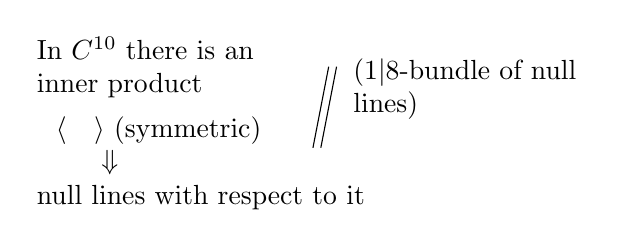
\begin{tikzpicture}
\node[anchor=west,text width=3.4cm] at (0,.27) {In $\mathbb C^{10}$ there is an inner product};
\node[anchor=west] at (.24,-.53) {$\langle\quad\rangle$ (symmetric)};
\node at (1.05,-.94) {$\Downarrow$};
\node[anchor=west] at (0,-1.38) {null lines with respect to it};
\draw (3.63,-.75)--(3.83,.28) (3.73,-.75)--(3.93,.28);
\node[anchor=west,text width=2.90cm] at (4.02,0) {($1|8$-bundle of null lines)};
\end{tikzpicture}}\endgroup}}
\end{GelfandAdjacentEvidence}
\begin{GelfandAdjacentEvidence}{GELFAND-P001199}{4}


[In the left margin:] \uwave{A. Goncharov.}

$SO(10)$ acts on $(\mathbb C^{10},\langle\, ,\,\rangle)$

$V_0\oplus V_1$,\quad $V_1$ --- spinor representation of the group $SO(10)$.
\SourceFigure{GELFAND-P001199}{spinor-group}{The line about the spinor representation reads $SO(10)$.}
\end{GelfandAdjacentEvidence}
\begin{GelfandAdjacentEvidence}{GELFAND-P001199}{5}


$\dim V_1=16$

Subspaces of dim. $(1,8)$: $L_0+L_1$

$L_0$ --- a null line in $\mathbb C^{10}$ $\Longrightarrow$
subgroup $SO(8)\subset SO(10)$

[Below the right-hand side:]
(in the stabilizer of the line $L_0$)

(its semisimple part --- $SO(8)$)

This is the group of rotations preserving $L_0$ and the orthogonal complement (which contains it)

$\Longrightarrow$ obtain rotations of the quotient space.

Now the spinor representation
\Unclear{GELFAND-P001199}{last-group-overwrite}{The mark before $SO(10)$ is heavily overwritten. It may be the Russian preposition “в” (in).}
\end{GelfandAdjacentEvidence}

$SO(10)$ restrict to $SO(8)$; obtain 2 invariant subspaces (8-dimensional)


\Needspace{7\baselineskip}
\begin{GelfandAdjacentEvidence}{GELFAND-P001200}{1}
\SourcePage{GELFAND-P001200}{59}
$\Longrightarrow$ 2 families of subspaces.

[Crossed out: illegible letters\textsuperscript{?}.]
\Unclear{GELFAND-P001200}{top-cancellation}{illegible letters}
\end{GelfandAdjacentEvidence}
\begin{GelfandAdjacentEvidence}{GELFAND-P001200}{2}

Consider the integrability condition for a connection along [inserted above: these] subspaces. This is a linear condition on the curvature, agreeing with the equations written earlier in a different context.

\begin{center}--- \(\cdot\) ---\end{center}
\uwave{Spinor representation.}

\[
e_1,\ldots,e_{10}:\qquad e_i e_k+e_k e_i=2\delta_{ik}I
\]
and the ring they generate

[At right, beyond a double vertical stroke:]
\[
x\cdot y+y\cdot x=(x,y)I
\]
\SourceFigure{GELFAND-P001200}{clifford-normalization}{In the formula to the right of the stroke, $x\cdot y+y\cdot x=(x,y)I$ is written without a factor of $2$.}
\end{GelfandAdjacentEvidence}
\begin{GelfandAdjacentEvidence}{GELFAND-P001200}{3}


Dim. of the ring: $e_1,\ldots,e_{10};\quad e_i e_k,\quad e_i e_j e_k$
\qquad $(e_i^2=I)$

In all $\dim=2^{10}$; it is simple (— isomorphic to a matrix ring).

[Under “matrix”:] $2^5\times2^5$

Obtain a representation of dimension 32.

$A\in SO(10)$ preserves the formulas $\Longrightarrow$ an automorphism of the matrix ring, and it is inner $\Longrightarrow$

$\Longrightarrow$ a representation arises.

\begin{center}--- \(\cdot\) ---\end{center}
\uwave{Curvature on the subspaces} $=0$ $\Longleftrightarrow$
\uwave{generalized self-dual Yang--Mills equation}.

\uwave{Ordinary Y.-M.}: dimensions 4 and 2.

\begin{center}--- \(\cdot\) ---\end{center}
\SourceFigure{GELFAND-P001200}{projective-quadric-diagram}{%
\par\smallskip
{\color{black}\begingroup\color{black}\GelfandFitDiagram{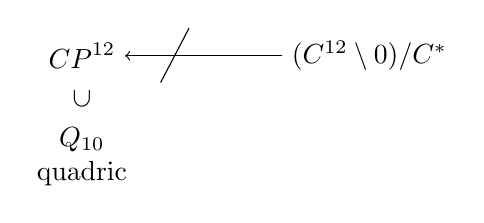
\begin{tikzpicture}
\node (projective) at (0,0) {$\mathbb{CP}^{12}$};
\node (quotient) at (3.65,0) {$({\mathbb C}^{12}\setminus0)/\mathbb C^*$};
\draw[->] (quotient)--(projective);
\draw (1.00,-.34)--(1.36,.35);
\node at (0,-.55) {\rotatebox{90}{$\subset$}};
\node at (0,-1.06) {$Q_{10}$};
\node at (0,-1.49) {quadric};
\end{tikzpicture}}\endgroup}%
\par The final exponent digit on $\mathbb{CP}$ is overwritten. The reading $12$ is tentative, possibly $11$. A diagonal stroke crosses the arrow. Its role is uncertain.}
\end{GelfandAdjacentEvidence}
\begin{GelfandAdjacentEvidence}{GELFAND-P001200}{4}


[To the right of $Q_{10}$:]
there is some covering supermn-zie [source abbr.]\textsuperscript{?}.
\Unclear{GELFAND-P001200}{super-direction-word}{Provisional reading: “supermn-zie.” The expansion of the abbreviation is uncertain.}
\end{GelfandAdjacentEvidence}
\begin{GelfandAdjacentEvidence}{GELFAND-P001200}{5}


\begin{center}--- \(\cdot\) ---\end{center}
\uwave{Radon--Penrose transform.}

$\mathbb{CP}^3$; lines in $\mathbb{CP}^3$ form $G(2,4)$
(2-dimensional subspaces of $\mathbb C^4$)

\SourceFigure{GELFAND-P001200}{radon-penrose-diagram}{%
\par\smallskip
{\color{black}\begingroup\color{black}\GelfandFitDiagram{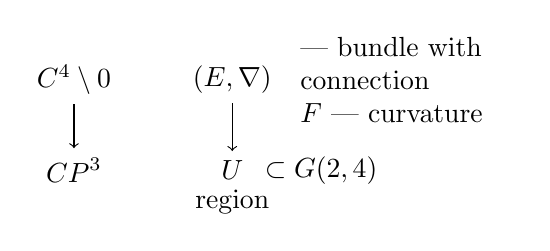
\begin{tikzpicture}
\node (affine) at (0,0) {$\mathbb C^4\setminus0$};
\node (proj) at (0,-1.15) {$\mathbb{CP}^3$};
\node (connection) at (2.01,0) {$(E,\nabla)$};
\node (region) at (2.01,-1.15) {$U$};
\node[anchor=west] at (2.30,-1.15) {$\subset G(2,4)$};
\node at (2.01,-1.55) {region};
\draw[->] (affine)--(proj);
\draw[->] (connection)--(region);
\node[anchor=west,text width=2.7cm] at (2.75,0)
  {--- bundle with connection\\$F$ --- curvature};
\end{tikzpicture}}\endgroup}}
\end{GelfandAdjacentEvidence}
\begin{GelfandAdjacentEvidence}{GELFAND-P001200}{6}


$\alpha$-planes in $T_xU$: there is a quadratic cone defined by the inner product.

In it [inserted above the line: 2] families of 2-dimensional [crossed out:
illegible letters\textsuperscript{?}]
\Unclear{GELFAND-P001200}{cone-cancellation}{illegible letters}
\end{GelfandAdjacentEvidence}

subspaces. Choose one of the families.

$F|_{\Pi_\alpha}=0$ $\Longleftrightarrow$ the bundle is called \uwave{self-dual}.

$G(2,4)$ has rank 2 (first after spheres). To match a pair of points one needs to specify 2 numbers (one on a sphere).

Curvature $=0$ $\Longrightarrow$ self-dual Y.-M. equation.

$\rightsquigarrow$ another bundle over $\mathbb{CP}^3$;
$\alpha$-surface — integral subset; the bundle is trivialized $\Longrightarrow$ it suffices to take the fibre over 1 point.

[At right, beyond a double vertical stroke:] Now a bundle without connection on another set.


\Needspace{7\baselineskip}
\begin{GelfandAdjacentEvidence}{GELFAND-P001201}{1}
\SourcePage{GELFAND-P001201}{unlabelled}
\underline{V.I. Arnold.} \underline{On} [inserted above: (some)] \underline{special functions arising in bifurcation theory.}

$H$ --- a polynomial

$H(x,y)=c$ --- a family of algebraic curves (real)

$\omega=P\,dx+Q\,dy$ --- a form ($P,Q$ --- polynomials)
\[
\oint_{H=c}\omega=I(c)
\]
How many zeros are there for the integral $I(c)$?

In one special case this is solved completely.

\underline{Theorem} (German Petrov-Tan’kin)
\SourceFigure{GELFAND-P001201}{theorem-name}{German Petrov-Tan’kin}
\end{GelfandAdjacentEvidence}
\begin{GelfandAdjacentEvidence}{GELFAND-P001201}{2}


5th-year student, vygn.\textsuperscript{?} from the university
\Unclear{GELFAND-P001201}{student-note}{The abbreviation is provisionally read as “vygn.”}
\end{GelfandAdjacentEvidence}
\begin{GelfandAdjacentEvidence}{GELFAND-P001201}{3}

\[
H=\frac{y^2}{2}+\underset{\text{a polynomial}}{P_3(x)}
\]
$c$ varies in the interval with ovals
\SourceFigure{GELFAND-P001201}{oval-word}{ovals}
\end{GelfandAdjacentEvidence}
\begin{GelfandAdjacentEvidence}{GELFAND-P001201}{4}


$\operatorname{deg}P\le n,\quad\operatorname{deg}Q\le n.$

\SourceFigure{GELFAND-P001201}{phase-figure}{%
\par\smallskip
{\color{black}\begingroup\color{black}\GelfandFitDiagram{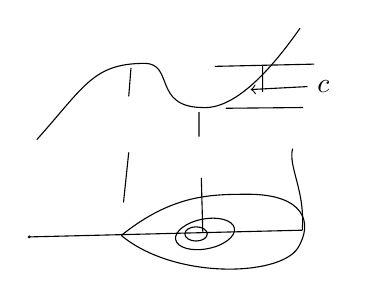
\begin{tikzpicture}[x=.95cm,y=.95cm]
\draw (.12,2.02) .. controls (.75,2.72) and (.87,3.04) .. (1.56,3.04)
      .. controls (1.96,3.04) and (1.67,2.46) .. (2.33,2.45)
      .. controls (2.75,2.42) and (3.22,2.91) .. (3.64,3.51);
\draw (2.50,3.00)--(3.83,3.03) (2.65,2.44)--(3.68,2.45)
      (3.14,3.01)--(3.14,2.66);
\draw[<-] (2.98,2.69)--(3.74,2.73) node[right] {$c$};
\draw (1.38,2.98)--(1.35,2.60) (2.29,2.39)--(2.29,2.06)
      (1.35,1.85)--(1.28,1.18) (2.32,1.51)--(2.34,.79)
      (3.54,1.90) .. controls (3.48,1.65) and (3.71,1.35) .. (3.67,.81);
\draw (.02,.72)--(3.67,.81);
\fill (.02,.72) circle (.021);
\draw (1.25,.74) .. controls (1.95,1.30) and (2.47,1.29) .. (2.98,1.29)
      .. controls (3.67,1.28) and (3.83,.93) .. (3.61,.57)
      .. controls (3.36,.19) and (1.96,.15) .. (1.25,.74);
\draw[rotate around={11:(2.37,.76)}] (2.37,.76) ellipse (.40 and .20);
\draw (2.25,.76) ellipse (.15 and .095);
\end{tikzpicture}}\endgroup}%
\par The thin vertical strokes between the curves are broken in places.}
\end{GelfandAdjacentEvidence}
\begin{GelfandAdjacentEvidence}{GELFAND-P001201}{5}


$\dim\{I\}=n$ (count using the Newton polyh.\textsuperscript{?})
\Unclear{GELFAND-P001201}{newton-abbreviation}{Newton polyh.}
\end{GelfandAdjacentEvidence}
\begin{GelfandAdjacentEvidence}{GELFAND-P001201}{6}


(the integrals are functions of $c$. They form a vector space since one can add the forms $\omega$)

\tikz{\node[draw,circle] {!};} \uwave{Assertion:} \uwave{number of zeros}
$\overset{\text{of any function considered}}{<n}$ (if it is $\ne0$)

the functions satisfy a Picard--Fuchs equation (Gauss--Manin connection)

\uwave{Comment:} $\forall f_1,\ldots,f_N$ the combination
$c_1f_1+\cdots+c_Nf_N$ has $N-1$ zeros
(if linearly independent)
\SourceFigure{GELFAND-P001201}{linear-combination-claim}{The wording reads “has $N-1$ zeros”. No inequality sign is visible here.}
\end{GelfandAdjacentEvidence}
\begin{GelfandAdjacentEvidence}{GELFAND-P001201}{7}


If the number of zeros is $<\dim$, the system is called \uwave{Chebyshev}

(\uwave{nonoscillation})

\uwave{Question:} relation to oscillation theorems?
\Unclear{GELFAND-P001201}{question-cancellation}{A short line beneath “Question” is hatched over. No letters can be read with certainty.}
\end{GelfandAdjacentEvidence}
\begin{GelfandAdjacentEvidence}{GELFAND-P001201}{8}


\begin{center}--- \(\cdot\) ---\end{center}

\uwave{Counting $\dim$}: $\int=0$ if a) an exact differential

b) multiply something by $H-c$.

\underline{Using the Newton polyhedron to compute dimensions}

\[
f=x^3+y^4;\qquad
\mathbb C[[x,y]]/(\tfrac{\partial f}{\partial x},\tfrac{\partial f}{\partial y})
\]

\SourceFigure{GELFAND-P001201}{newton-left-figure}{%
\par\smallskip
{\color{black}\begingroup\color{black}\GelfandFitDiagram{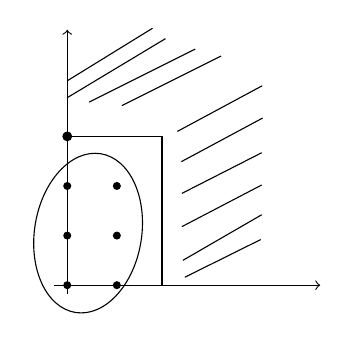
\begin{tikzpicture}[x=.63cm,y=.63cm]
\draw[->] (-.27,0)--(5.1,0);
\draw[->] (0,-.18)--(0,5.15);
\draw (0,3)--(1.91,3)--(1.91,0);
\draw (0,4.12)--(1.72,5.18) (0,3.78)--(1.98,4.97)
      (.44,3.69)--(2.58,4.76) (1.10,3.62)--(3.10,4.62)
      (2.22,3.10)--(3.93,4.02) (2.30,2.49)--(3.94,3.37)
      (2.31,1.85)--(3.92,2.67) (2.31,1.18)--(3.92,2.02)
      (2.33,.50)--(3.92,1.42) (2.37,.16)--(3.90,.92);
\foreach \x in {0,1}{\foreach \y in {0,1,2}{\fill (\x,\y) circle (.081);}}
\fill (0,3) circle (.10);
\draw[rotate around={-9:(.42,1.05)}] (.42,1.05) ellipse (1.08 and 1.62);
\end{tikzpicture}}\endgroup}}
\end{GelfandAdjacentEvidence}
\begin{GelfandAdjacentEvidence}{GELFAND-P001201}{9}


basis of the quotient space. $\dim=6$

$x^2y+y^4$

\SourceFigure{GELFAND-P001201}{newton-right-figure}{%
\par\smallskip
{\color{black}\begingroup\color{black}\GelfandFitDiagram{\begin{tikzpicture}[x=.60cm,y=.60cm]
\draw (-.55,0)--(6.05,0) (0,-.06)--(0,3.32);
\draw (0,.41)--(.11,.48) (.64,-.05)--(.64,.08) (1.26,-.05)--(1.26,.06);
\draw (-.13,1.18) rectangle (.14,1.46) (1.77,-.14) rectangle (2.10,.13);
\draw (-.08,1.22)--(.06,1.41) (1.83,-.09)--(2.04,.07);
\draw (.64,1.35) circle (.14) (2.56,0) circle (.16);
\draw (.56,1.27)--(.65,1.45) (.65,1.26)--(.71,1.41)
      (2.46,-.10)--(2.53,.11) (2.55,-.11)--(2.62,.13) (2.63,-.07)--(2.68,.07);
\draw (.48,.56)--(.65,.80)--(.80,.57)--cycle;
\node[anchor=west] at (.20,-.69) {$\Rightarrow$ \uwave{basis}.};
\end{tikzpicture}}\endgroup}%
\par The interior strokes in the squares and circles are schematic. Their reading remains uncertain.}
\end{GelfandAdjacentEvidence}



\Needspace{7\baselineskip}
\begin{GelfandAdjacentEvidence}{GELFAND-P001202}{1}
\SourcePage{GELFAND-P001202}{60}
\underline{A. Zelevinsky.} On “the most beautiful result in pure math.”

(Jacobi triple product)
\[
(1)\quad
\sum_{r=-\infty}^{\infty}z^r q^{r^2}
=\prod_{k=1}^{\infty}(1-q^{2k})(1+q^{2k-1}z)(1+q^{2k-1}z^{-1})
\]
(Jacobi triple product)
\[
\Vert
\]
\[
(1;q^2)_\infty(-zq^{-1};q^2)_\infty(-z^{-1}q^{-1};q^2)_\infty
\]
\SourceFigure{GELFAND-P001202}{pochhammer-product}{The first factor has $1$ before the semicolon. The next two factors have $q^{-1}$.}
\end{GelfandAdjacentEvidence}
\begin{GelfandAdjacentEvidence}{GELFAND-P001202}{2}


Here
\[
(a;q)_\infty:=\prod_{n=0}^{\infty}(1-aq^n)
\]
!! Follows from \uwave{Ramanujan’s identity.}

\uwave{Combinatorial proof}

Move the first product to the left-hand side
\[
(2)\quad
\left(\sum_{r=-\infty}^{\infty}z^r q^{r^2}\right)
\prod_{k=1}^{\infty}(1-q^{2k})^{-1}
=\prod_{k=1}^{\infty}(1+q^{2k-1}z)(1+q^{2k-1}z^{-1})
\]
\Unclear{GELFAND-P001202}{equation-two-cancellation}{A mark above $z^r$ on the left of (2) is heavily crossed out.}
\end{GelfandAdjacentEvidence}
\begin{GelfandAdjacentEvidence}{GELFAND-P001202}{3}


Only the coefficient at the following type of monomial is nonzero $\underline{z^r q^{r^2+2n}}$

(on the left and on the right)

$={}$ number of partitions of $n$ into summands $=p(n)$

(on the left)

(3) \uwave{On the right:} exponents
\[
\alpha_1>\alpha_2>\cdots>\alpha_s>0
\]
odd
\[
\beta_1>\beta_2>\cdots>\beta_t>0
\]
\Unclear{GELFAND-P001202}{beta-inequalities}{The final comparison reads $>$. The three preceding signs are heavily retraced. Their provisional reading is $>$, with $\geq$ also possible.}
\end{GelfandAdjacentEvidence}
\begin{GelfandAdjacentEvidence}{GELFAND-P001202}{4}

\[
\sum\alpha_j+\sum\beta_i=r^2+2n,\qquad \underline{\underline{s-t=r}}
\]
[Two diverging strokes from “odd” point toward the $\alpha$ and $\beta$ lines. Vertical strokes flank the lines.]

\SourceFigure{GELFAND-P001202}{both-descriptions}{Both the one and the other}
\end{GelfandAdjacentEvidence}
\begin{GelfandAdjacentEvidence}{GELFAND-P001202}{5}

(Z.L. Leibenzon) --- combinatorial description of the set:
\SourceFigure{GELFAND-P001202}{leibenzon-name}{Z.L. Leibenzon}
\end{GelfandAdjacentEvidence}
\begin{GelfandAdjacentEvidence}{GELFAND-P001202}{6}

\[
00000\,1\,0000\,1\,00\,111111
\]
infinite words (\uwave{linkages})

[Crossed out: on the left\textsuperscript{?}]
\Unclear{GELFAND-P001202}{cancelled-left-word}{on the left}
\end{GelfandAdjacentEvidence}

first infinitely many $0$; then a jumble; then \underline{strokes}

(infinitely many)

Height: $h(A)$ --- number of inversions $\underbrace{1\,0}$ --- arbitrarily far apart

$\underline{h(A)=n}\quad\Rightarrow$ number of elements $p(n)$

--- parametrized by tuples of the form (3).

\underline{1st method}
\[
0000\,1\,0\,111\qquad\text{--- height }1
\]
$p(n)$ --- take the leftmost stroke and count zeros after it, and so on.

\underline{2nd method}

The gaps have a [above “number”: (natural)] number:
(number of $1$ on the left) $-$ (number of $0$ on the right)

\uwave{The number} varies from $-\infty$ to $+\infty$ !! (throughout!)


\Needspace{7\baselineskip}
\begin{GelfandAdjacentEvidence}{GELFAND-P001203}{1}
\SourcePage{GELFAND-P001203}{unlabelled}
\uwave{Arnold’s remark:}

Let us draw:

$0$ --- a step to the right

$1$ --- a step up

\SourceFigure{GELFAND-P001203}{young-step-diagram}{%
\par\smallskip
{\color{black}\begingroup\color{black}\GelfandFitDiagram{\begin{tikzpicture}[x=.48cm,y=.38cm]
\draw (-4.5,0)--(0,0)--(0,1)--(2,1)--(2,2)--(3,2)--(3,4)--(4,4)--(4,7.3);
\draw[line width=1.4pt] (3,4)--(4,4);
\node at (-.35,-.42) {$0$};
\node at (-.27,.50) {$1$};
\node at (.50,1.40) {$0$};
\node at (1.50,1.40) {$0$};
\node at (2.30,1.55) {$1$};
\node at (2.52,2.44) {$0$};
\node at (3.32,2.53) {$1$};
\node at (3.32,3.53) {$1$};
\node at (3.50,4.44) {$0$};
\node at (4.32,4.59) {$1$};
\node at (4.32,5.59) {$1$};
\node at (4.32,6.63) {$1$};
\end{tikzpicture}}\endgroup}}
\end{GelfandAdjacentEvidence}
\begin{GelfandAdjacentEvidence}{GELFAND-P001203}{2}


Young diagram

the function $\underline{x-y}$ \uwave{numbers} all

Consider the gap numbered $r$.

We characterize the linkage as follows:

the distance from the gap to the sticks, \textit{[beneath the word, with a brace: lying to the left]} $\Vert$ \uwave{odd numbers}.

--- ″ --- the circles. \textit{[beneath the word, with a brace: lying to the right]}
\[
\sum\alpha_j+\sum\beta_j=r^2+2n
\]
from the area under the curve.

\Needspace{7\baselineskip}
16/IX--85  \underline{Gelfand Seminar.}

\underline{Zelevinsky} (\underline{and Beilinson}) as reported by \uwave{M.-F. Vigneras} (Marie-France Vigneras)
\Unclear{GELFAND-P001203}{name-aside}{Above “to” is a parenthetical note, provisionally read as “Ma’tici.” There is a separate raised stroke after a.}
\end{GelfandAdjacentEvidence}
\begin{GelfandAdjacentEvidence}{GELFAND-P001203}{3}


1) on the work “From \(\mathrm{GL}(2,\mathbb Q\sqrt d)\) to \(\mathrm{GSp}(4,\mathbb Q)\)” (M.-F. Vigneras)
\Unclear{GELFAND-P001203}{lifting-field-notation}{The first letter in the field notation is overwritten and is read as \(\mathbb Q\sqrt d\).}
\end{GelfandAdjacentEvidence}
\begin{GelfandAdjacentEvidence}{GELFAND-P001203}{4}


Construction of a correspondence between representations.

(lifting)

On passing to a $p$-adic field

this makes it possible to verify for \(\mathrm{GSp}(4,F)\) some Langlands conjecture on functoriality.

\textit{[At right, with a pointer to \(\mathrm{GSp}\):]} symplectic similitudes (preserve the symplectic form up to a scalar)

\textit{[Below \(F\):]} $p$-adic

2) \uwave{Rallis, Piatetski-Shapiro and others}
\[
L(s,\pi_1\times\pi_2\times\pi_3),\quad
\text{where }\pi_j\text{ --- representations of }\mathrm{GL}_2(F)
\]
3) According to Jacket “\underline{How} \underline{to use} the trace formula?”
\SourceFigure{GELFAND-P001203}{latin-surname}{The surname in the manuscript reads “Jacket.”}
\end{GelfandAdjacentEvidence}
\begin{GelfandAdjacentEvidence}{GELFAND-P001203}{5}


The latest important result is the Paley--Wiener theorem,
\Unclear{GELFAND-P001203}{cancelled-theorem-phrase}{Possible beginning of the crossed-out words after the theorem name: “ob \ldots.”}
\end{GelfandAdjacentEvidence}
\begin{GelfandAdjacentEvidence}{GELFAND-P001203}{6}

proved by Kazhdan and Bernstein.

\SourceFigure{GELFAND-P001203}{result-abbreviation}{The abbreviation at the start of the line is read as “latest.”}
\end{GelfandAdjacentEvidence}
\begin{GelfandAdjacentEvidence}{GELFAND-P001203}{7}


\textit{[In an oval linked to the name of the result:]} on representations over \(F\)

\(G\) --- a reductive $p$-adic group (e.g. \(\mathrm{GL}_n\))

\(H^{\bullet}(G)\) --- [Inserted above the dash: alg.] locally constant, compactly supported functions on \(G\).
\SourceFigure{GELFAND-P001203}{hecke-superscript}{The raised mark after \(H\) is read as a dot.}
\end{GelfandAdjacentEvidence}
\begin{GelfandAdjacentEvidence}{GELFAND-P001203}{8}

\SourceFigure{GELFAND-P001203}{algebra-insertion}{“Alg.” is inserted above the dash, with a curved mark linking it to the line.}
\end{GelfandAdjacentEvidence}
\begin{GelfandAdjacentEvidence}{GELFAND-P001203}{9}


\textit{[To the right of the vertical stroke:]} locally constant functions take the place of \(C^\infty\) functions

From \(f\) we construct:
\[
\pi\longrightarrow\operatorname{tr}\pi(f)
\]
--- a function on \(\operatorname{Irr}G\)

Here
\[
\pi(f)=\int_G f(g)\pi(g)\,dg
\]
\underline{The theorem} (Paley--Wiener, according to K.-B.) describes all such functions

Irreducible representations divide into sheets and families: from \(\rho\in\operatorname{Irr}M\) one constructs

\(M\subset G\)
\[
\pi\in\mathrm{JH}\;\operatorname{Ind}_{\underline{P}}^{G}\rho
\]
(Jordan--Hölder series)
\Unclear{GELFAND-P001203}{induction-subscript}{There is a stroke under the subscript. The retraced letter is provisionally read as \(P\).}
\end{GelfandAdjacentEvidence}
\begin{GelfandAdjacentEvidence}{GELFAND-P001203}{10}


\(\Vert\) each family acquires a structure

\(M\) --- the Levi subgroup of a parabolic subgroup of \(G\)

(semisimple part)

character of an irreducible representation \(\Leftrightarrow\) \underline{algebraicity} of a certain function

Idea in the real \textit{[below “real,” circled: and complex?]} case: ubyv.\textsuperscript{?} on \(\forall\) Cartan subalgebra
\Unclear{GELFAND-P001203}{final-verb}{Possible readings of the abbreviation are “ubyv.” and “ubiv.”}
\end{GelfandAdjacentEvidence}



\Needspace{7\baselineskip}
\begin{GelfandAdjacentEvidence}{GELFAND-P001204}{1}
\SourcePage{GELFAND-P001204}{61}
\underline{M.-F. Vigneras.}\quad (on the same topic, but more precisely)
\Unclear{GELFAND-P001204}{upper-aside-final}{The note ends with the provisional abbreviation “tochn.” for “precisely.”}
\end{GelfandAdjacentEvidence}
\begin{GelfandAdjacentEvidence}{GELFAND-P001204}{2}


\(G\) reductive \(p\)-adic group (e.g., \(\mathrm{GL}_n\))
\begin{equation*}
\coprod_{(M,\rho)}\{\rho\chi\}^{W}=\operatorname{Irr}G \tag{1}
\end{equation*}
\textit{[Labels with pointers:]} \(M\) --- standard reductive subgroup,
\(\rho\) --- irreducible cuspidal representation,
\(\chi\) --- unramified character,
\(W\) --- up to the action of the Weyl group.
\SourceFigure{GELFAND-P001204}{upper-m-caption}{The first line of the label for \(M\) is read as the abbreviation for “standard.”}
\end{GelfandAdjacentEvidence}
\begin{GelfandAdjacentEvidence}{GELFAND-P001204}{3}


\(\{\rho\chi\}^{W}\) --- finite-dimensional algebraic set (\(\text{over }\mathbb C\)).

from \(f\in H(G)\) one constructs a function on [inserted: the set (1)]
\[
\pi\longrightarrow\operatorname{trace}\operatorname{ind}_{M}^{G}\rho\chi(f)
\]
Conditions

a) algebraic on \(\forall\) such set

b) supported on finitely many of them

\Needspace{6\baselineskip}
\underline{\underline{Beilinson.}}
\Unclear{GELFAND-P001204}{middle-beilinson-cancel}{The words below the heading are crossed out and cannot be read with certainty.}
\end{GelfandAdjacentEvidence}
\begin{GelfandAdjacentEvidence}{GELFAND-P001204}{4}


Representations of \(\mathrm{GSp}(4,\mathbb Q)\) --- ?
\[
W_{\mathbb Q_p}\subset\operatorname{Gal}(\overline{\mathbb Q}_p/\mathbb Q_p)
\]
\[
\operatorname{Irr}\mathrm{GSp}(4,\mathbb Q)
\longrightarrow \text{representations of the Weil--Deligne group}
\]
\Unclear{GELFAND-P001204}{middle-wd-sign}{A mark after the arrow, before “representations,” is heavily retraced. Its reading and role are uncertain.}
\end{GelfandAdjacentEvidence}
\begin{GelfandAdjacentEvidence}{GELFAND-P001204}{5}


\textit{[With a pointer to the right-hand side of the arrow:]} the inverse image of \(\forall\) point is finite (\(L\) packet)
\[
\mathrm{GL}(2,\mathbb Q(\sqrt d))\longrightarrow\mathrm{GO}(4)
\]
\[
\left\{x\in M(2,\mathbb Q(\sqrt d)):x=\bar x\right\}
\qquad
x=\begin{pmatrix}a&b\\\bar b&d\end{pmatrix}
\]
\SourceFigure{GELFAND-P001204}{middle-hermitian-condition}{The condition reads \(x=\bar x\), with no visible transpose sign.}
\end{GelfandAdjacentEvidence}
\begin{GelfandAdjacentEvidence}{GELFAND-P001204}{6}


\(\det\) --- canonical quadratic form\quad (it is rational)
\[
x\longmapsto gx\bar g^{t}\qquad\text{preserves this condition}
\]
(analogue of the spinor representation)

Weil representation: representation of \(\mathrm{GO}(4)\times\mathrm{GSp}(4)\)

it is realized in \(\theta\) functions

\Needspace{6\baselineskip}
\underline{\underline{B. Feigin.}}\qquad \underline{On strings}
\Unclear{GELFAND-P001204}{lower-theory-cancel}{The crossed-out word before “String theory” remains unresolved.}
\end{GelfandAdjacentEvidence}
\begin{GelfandAdjacentEvidence}{GELFAND-P001204}{7}


String theory is the statistics of surfaces.

Quantum mechanics studies a space with a Lagrangian. The action depends on the trajectory.

Strings: a surface takes the place of a trajectory.

\(\mathcal E\) --- a Riemann surface; consider the space \(\mathbb R^d\)

A trajectory is a map
\[
\underset{x_1,\ldots,x_d}{\{\mathcal E\longrightarrow\mathbb R^d\}}.
\]
\uwave{Idea:} all elementary particles are described by maps from \(\mathcal E\) to the superspace \(\mathbb R^{10/m}\)
\SourceFigure{GELFAND-P001204}{string-super-dimension}{The exponent shows a slash and \(m\): \(10/m\).}
\end{GelfandAdjacentEvidence}
\begin{GelfandAdjacentEvidence}{GELFAND-P001204}{8}


The motion of a circle gives a surface
\SourceFigure{GELFAND-P001204}{circle-worldsheet}{%
\par\smallskip
{\color{black}\begingroup\color{black}\GelfandFitDiagram{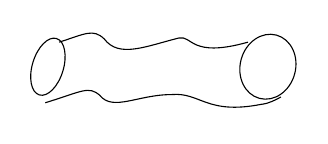
\begin{tikzpicture}[x=1.1cm,y=1.04cm]
\draw[rotate around={-17:(0,0)}] (0,0) ellipse (.18 and .36);
\draw[rotate around={-15:(2.54,0)}] (2.54,0) ellipse (.32 and .40);
\draw (.13,.30) .. controls (.43,.40) and (.52,.47) .. (.65,.34)
 .. controls (.82,.10) and (1.13,.25) .. (1.51,.35)
 .. controls (1.67,.39) and (1.64,.10) .. (2.31,.30);
\draw (-.03,-.44) .. controls (.40,-.30) and (.47,-.23) .. (.60,-.35)
 .. controls (.75,-.55) and (1.04,-.34) .. (1.43,-.34)
 .. controls (1.76,-.31) and (1.83,-.59) .. (2.46,-.46)
 .. controls (2.55,-.45) and (2.62,-.41) .. (2.69,-.37);
\end{tikzpicture}}\endgroup}}
\end{GelfandAdjacentEvidence}


The classical analogue is crystal growth.


\Needspace{7\baselineskip}
\begin{GelfandAdjacentEvidence}{GELFAND-P001205}{1}
\SourcePage{GELFAND-P001205}{unlabelled}
Lagrangian:
\begin{equation*}
\mathcal L=\int\text{[crossed out]}\,
(\det g_{ij})^{1/2}\,d\sigma\,d\tau
\qquad \text{(Nambu Lagrangian)} \tag{1}
\end{equation*}
\Unclear{GELFAND-P001205}{upper-lagrangian-cancel}{The passage crossed out immediately after the integral sign remains unresolved.}
\end{GelfandAdjacentEvidence}
\begin{GelfandAdjacentEvidence}{GELFAND-P001205}{2}

(area in the induced metric)

We need to consider the Feynman integral.
\[
X:\mathcal E\hookrightarrow\mathbb R^d
\]
Another way to write (1):
\begin{equation*}
\mathcal L(X)=\int d\sigma\,d\tau
\left[
\left(\frac{\partial X}{\partial\sigma}\right)^2
\left(\frac{\partial X}{\partial\tau}\right)^2
-\left(\frac{\partial X}{\partial\sigma}\cdot
\frac{\partial X}{\partial\tau}\right)^2
\right]^{1/2} \tag{1'}
\end{equation*}
Feynman integral
\begin{equation*}
\int e^{\beta\mathcal L(X)}\,\mathcal D X \tag{2}
\end{equation*}
There are two approaches: via integrals and via ordinary operators (!). A correspondence has now been established.

\Needspace{7\baselineskip}
\uwave{Polyakov:} another continuum integral

\(\widetilde X\) --- [inserted: a space] whose elements are pairs

1) \(X:\mathcal E\longrightarrow\mathbb R^d\)

2) \(g_{ij}\) on \(\mathcal E\) (a Riemannian metric on \(\mathcal E\))

Polyakov Lagrangian:
\begin{equation*}
\text{[crossed out]}\,
\mathcal L=\text{\ae}\int(\det g_{ij})^{1/2}
+\int\frac{\partial X_i}{\partial\xi_\alpha}
\frac{\partial X_i}{\partial\xi_\beta}g^{\alpha\beta}
\overset{\text{[inserted]}}{\sqrt g}\,d\xi_1\,d\xi_2
\tag{3}
\end{equation*}
\Unclear{GELFAND-P001205}{lower-lagrangian-cancel}{The crossed-out mark before \(\mathcal L\) remains unresolved.}
\end{GelfandAdjacentEvidence}
\begin{GelfandAdjacentEvidence}{GELFAND-P001205}{3}

\Unclear{GELFAND-P001205}{lower-lagrangian-coefficient}{The coefficient before the first integral is represented by its “æ”-like shape. The letter remains unidentified.}
\end{GelfandAdjacentEvidence}
\begin{GelfandAdjacentEvidence}{GELFAND-P001205}{4}

\SourceFigure{GELFAND-P001205}{polyakov-measure}{\(\sqrt g\) is inserted above the line. The overwritten subscripts in \(d\xi_1\,d\xi_2\) are read as \(1,2\).}
\end{GelfandAdjacentEvidence}


[Inserted: To it] the calculation technique applies

Procedure: fix \(g_{ij}\) and evaluate the integral over \(X\) --- it is quadratic.
\begin{center}--- \(\cdot\) ---\end{center}


\Needspace{7\baselineskip}
\begin{GelfandAdjacentEvidence}{GELFAND-P001206}{1}
\SourcePage{GELFAND-P001206}{62}
\underline{23.9.85}\quad\underline{Gelfand Seminar.}

\uwave{I.M.G.} \underline{Problem (for grade 9)}
What polyhedron results from cutting a 4-dimensional cube by a 3-dimensional hyperplane passing through the center and perpendicular to the main diagonal?

\underline{A. Beilinson.} \uwave{On a new series of papers by Piatetski-Shapiro and Rallis.}

functional equations of $L$-functions associated with automorphic forms

\(G\) --- a semisimple group over \(\mathbb Q\) (e.g., the group of matrices \(n\times n\))

\(G/\mathbb Q\).
\Unclear{GELFAND-P001206}{upper-gq-cancel}{The signs to the right of \(G/\mathbb Q\) are heavily crossed out.}
\end{GelfandAdjacentEvidence}
\begin{GelfandAdjacentEvidence}{GELFAND-P001206}{2}


\underline{Problem:} describe the representations of the adelic group \(G(A)\) in \(L^2(G(A)/G(\mathbb Q)\)
\SourceFigure{GELFAND-P001206}{upper-l2-parentheses}{The notation for the \(L^2\) space has one closing parenthesis after \(\mathbb Q\).}
\end{GelfandAdjacentEvidence}
\begin{GelfandAdjacentEvidence}{GELFAND-P001206}{3}


The corresponding representations are called \uwave{automorphic}.
\begin{center}--- \(\cdot\) ---\end{center}
\uwave{I.M.G.} \(\forall\) natural number can be written in the form
\[
a_0+a_1p+a_2p^2+\ldots+a_np^n
\]
Any rational number
\[
a_{-m}p^{-m}+a_1p^{-m+1}+\ldots+a_kp^k+
\]
\SourceFigure{GELFAND-P001206}{middle-rational-expansion}{The second term reads \(a_1p^{-m+1}\). A \(+\) follows \(a_kp^k\).}
\end{GelfandAdjacentEvidence}
\begin{GelfandAdjacentEvidence}{GELFAND-P001206}{4}


For example,
\[
\frac13=1+1\cdot2+1\cdot2^3+1\cdot2^5+\ldots
\]
\textit{[At right:]}
\[
\|a\|=p^{-n},\quad\text{if }a=p^nm,\quad(a,m)=1.
\]
\SourceFigure{GELFAND-P001206}{middle-coprimality}{The coprimality condition reads \((a,m)=1\).}
\end{GelfandAdjacentEvidence}
\begin{GelfandAdjacentEvidence}{GELFAND-P001206}{5}

\[
\underline{p=2}\quad\Rightarrow\quad
\|2\|=\frac12;\quad\|3\|=1,\quad\|4\|=\frac14,\quad
\left\|\frac12\right\|=2.
\]
\[
\text{Adeles}=\prod_p(\text{\(p\)-adic numbers})
\]
\SourceFigure{GELFAND-P001206}{middle-adeles-product}{The manuscript has “\(p\)-adic numbers,” with \(p\) below the product sign.}
\end{GelfandAdjacentEvidence}
\begin{GelfandAdjacentEvidence}{GELFAND-P001206}{6}

\begin{center}--- \(\cdot\) ---\end{center}
\[
\mathrm{SL}_2(\mathbb R)\supset\mathrm{SL}_2(\mathbb Z)\supset\Gamma_n
\]
\textit{[Label pointing to \(\Gamma_n\):]} matrices of order 2,
[crossed out: elem.?] that are congruent\textsuperscript{?} to \(1\) (matrix) \(\bmod n\).
\Unclear{GELFAND-P001206}{middle-matrices-cancel}{The abbreviation crossed out after “order” may read “elem.”}
\end{GelfandAdjacentEvidence}
\begin{GelfandAdjacentEvidence}{GELFAND-P001206}{7}

\Unclear{GELFAND-P001206}{middle-matrices-congruence}{The beginning reads “sravn.” The retraced ending is provisionally read as “-my,” giving “congruent.”}
\end{GelfandAdjacentEvidence}
\begin{GelfandAdjacentEvidence}{GELFAND-P001206}{8}

\[
\Gamma_{n_1}\supset\Gamma_{n_2}\quad\text{when }n_1\mid n_2
\]
\[
G(A)/G(\mathbb Q)=\varprojlim_n G(\mathbb R)/\Gamma_n.
\]
\(\Gamma_n\) acts on the upper half-plane \(H\); \(H/\Gamma_n\) ---
[crossed out: Riemann?] [inserted: a sphere] (with punctures)
\Unclear{GELFAND-P001206}{lower-surface-cancel}{The first crossed-out word may be “Riemann.” “A sphere” is inserted above the line.}
\end{GelfandAdjacentEvidence}
\begin{GelfandAdjacentEvidence}{GELFAND-P001206}{9}


\(H/\mathrm{SL}_2(\mathbb Z)\) --- a sphere with two punctures

\(H/\Gamma_2\) --- --- ″ --- three punctures
\SourceFigure{GELFAND-P001206}{lower-modular-quotients}{The first line says “a sphere with two punctures.”}
\end{GelfandAdjacentEvidence}
\begin{GelfandAdjacentEvidence}{GELFAND-P001206}{10}

\[
\pi_{G(A)}=\pi_{G(\mathbb R)}\otimes\pi_{G(\mathbb Q_2)}\otimes\ldots
\]
\begin{center}--- \(\cdot\) ---\end{center}
\uwave{I.M.G.} At \uwave{Sem. Bourbaki} there is a paper by \uwave{A. Connes}
\underline{on the relation between the topology of knots and invariants of factors}!!
\SourceFigure{GELFAND-P001206}{lower-knot-abbreviation}{The abbreviation before “knots” reads “top.”}
\end{GelfandAdjacentEvidence}
\begin{GelfandAdjacentEvidence}{GELFAND-P001206}{11}

\begin{center}--- \(\cdot\) ---\end{center}
It is enough to know the representations of the $p$-adic group.
\Unclear{GELFAND-P001206}{lower-padic-cancel}{The crossed-out mark at the end of the line remains unresolved.}
\end{GelfandAdjacentEvidence}
\begin{GelfandAdjacentEvidence}{GELFAND-P001206}{12}


Which occur in \(L^2(G(A)/G(\mathbb Q))\)? Far from all of them.

\uwave{Representations of} \(G(\mathbb Q_p)\).

The simplest are spherical, when there is a vector invariant under a [inserted: max] compact subgroup.
\[
G(\mathbb Q_p)/B(\mathbb Q_p)
\]
\SourceFigure{GELFAND-P001206}{borel-matrix-layout}{%
\par\smallskip
{\color{black}\(\displaystyle B=
\begin{pmatrix}
\ast&&&\\[-.45em]
&\ast&&\\[-.45em]
0&&\ast&\\[-.45em]
&&&\ast
\end{pmatrix}\)}}
\end{GelfandAdjacentEvidence}



\Needspace{7\baselineskip}
\begin{GelfandAdjacentEvidence}{GELFAND-P001207}{1}
\SourcePage{GELFAND-P001207}{unlabelled}

are indexed by unramified characters of the torus \(\chi_{nr}(T)\)
\(=\) points of the dual torus \(=T^0(\mathbb C)\) (complex points)
\Unclear{GELFAND-P001207}{top-character-subscript}{The subscript on \(\chi\) is provisionally read as \(nr\). The second glyph is uncertain.}
\end{GelfandAdjacentEvidence}
\begin{GelfandAdjacentEvidence}{GELFAND-P001207}{2}


(trivial on the intersection of the torus with the maximal compact subgroup)

Spherical representations of \(G(\mathbb Q_p)=T^0(\mathbb C)/W\)

unramified character \(\longrightarrow\) conjugacy class in the matrix group

\begin{center}--- \(\cdot\) ---\end{center}

Let \(G\) --- a split group (the maximal torus splits)

\(G^0\) --- dual group\qquad (\(G=\mathrm{GL}\Rightarrow G^0=\mathrm{GL}\))

\SourceFigure{GELFAND-P001207}{satake-parameter-diagram}{%
\par\smallskip
{\color{black}\begingroup\color{black}\GelfandFitDiagram{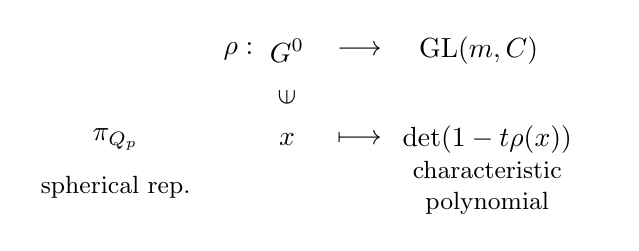
\begin{tikzpicture}[x=.78cm,y=.78cm]
\node at (2.00,1.45) {\(\rho:\)};
\node at (2.79,1.45) {\(G^0\)};
\node at (3.97,1.45) {\(\longrightarrow\)};
\node at (5.91,1.45) {\(\mathrm{GL}(m,\mathbb C)\)};
\node[rotate=90] at (2.79,.70) {\(\in\)};
\node at (.0,0) {\(\pi_{\mathbb Q_p}\)};
\node at (1.17,0) {\(\rightsquigarrow\)};
\node at (2.79,0) {\(x\)};
\node at (3.97,0) {\(\longmapsto\)};
\node at (6.05,0) {\(\det(1-t\rho(x))\)};
\node[align=center,text width=2.0cm,font=\small] at (.0,-.78) {spherical rep.};
\node[align=center,text width=2.9cm,font=\small] at (6.05,-.78) {characteristic polynomial};
\end{tikzpicture}}\endgroup}}
\end{GelfandAdjacentEvidence}
\begin{GelfandAdjacentEvidence}{GELFAND-P001207}{3}


Suppose that for \(\pi_{G(A)}\) almost all representations
[Inserted above the line: (of the local groups \(G(\mathbb Q_p)\))] are spherical
(all but finitely many)

\[
L(\pi,\rho,s)=\prod_p
\frac{1}{\det\left(1-p^{-s}\rho\left(
\underset{\substack{\vert\\\text{semisimple element}}}{x_{\pi_{\mathbb Q_p}}}
\right)\right)}
\]

\begin{center}--- \(\cdot\) ---\end{center}

\underline{Example}.
\[
\rho:\mathrm{GL}_1\underset{\text{identity}}{\longrightarrow}\mathrm{GL}_1
\quad\Rightarrow\quad
x\longmapsto\underset{\text{polynomial\textsuperscript{?}}}{1-tx}
\]
\Unclear{GELFAND-P001207}{example-polynomial-caption}{The abbreviation below \(1-tx\) is provisionally read as “mnogoch.” or “mnogochl.” (“polynomial”).}
\end{GelfandAdjacentEvidence}
\begin{GelfandAdjacentEvidence}{GELFAND-P001207}{4}

\Unclear{GELFAND-P001207}{example-cancelled-symbol}{The crossed-out mark before \(x=1\) remains unresolved.}
\end{GelfandAdjacentEvidence}
\begin{GelfandAdjacentEvidence}{GELFAND-P001207}{5}


\(x=1\Rightarrow L(\pi,\rho,s)=\prod_p\frac{1}{1-p^{-s}}\)
--- the Riemann \(\zeta\)-function.

\Needspace{7\baselineskip}
\underline{\underline{Feigin B.}}\qquad\underline{On strings (continued).}

\(\mathcal E\) --- a Riemann surface (a 2-dimensional set);
\(\mathbb R^d\) --- a space with the Minkowski metric
\(\langle\, , \,\rangle\) (1 negative square) or the Euclidean metric.

Consider the space [Inserted above the line: \(X\)] of smooth maps
\(\mathcal E\overset{x}{\longrightarrow}\mathbb R^d\)

[Inserted above the line: The map \(x\) induces]
on \(\mathcal E\) [crossed out] a Riemannian metric.
\Unclear{GELFAND-P001207}{metric-cancelled-word}{The crossed-out word after \(\mathcal E\) may start with the Russian letters “зад…”.}
\end{GelfandAdjacentEvidence}
\begin{GelfandAdjacentEvidence}{GELFAND-P001207}{6}


Let \(\xi_1,\xi_2\) --- coordinates [crossed out] on \(\mathcal E\).
\Unclear{GELFAND-P001207}{coordinates-cancelled-symbol}{The crossed-out writing between “coordinates” and “on” remains unresolved.}
\end{GelfandAdjacentEvidence}

\begin{equation*}
g_{ij}=\left(\frac{\partial x}{\partial\xi_i},
\frac{\partial x}{\partial\xi_j}\right)
\qquad \{g^{ij}\}=\{g_{ij}\}^{-1}
\tag{1}
\end{equation*}
Nambu Lagrangian:
\begin{equation*}
\mathcal L(x)=\int_{\mathcal E}\omega
=\int_{\mathcal E}\sqrt g\,d\xi_1\,d\xi_2,
\qquad g=\det\{g_{ij}\}
\tag{2}
\end{equation*}
(area of the surface in the Riemannian metric)


\Needspace{7\baselineskip}
\begin{GelfandAdjacentEvidence}{GELFAND-P001208}{1}
\SourcePage{GELFAND-P001208}{63}

Path integral
\begin{equation*}
\int e^{\frac{i}{h}\mathcal L(x)}\mathcal D x
\tag{3}
\end{equation*}
\Unclear{GELFAND-P001208}{exponential-coefficient}{The overwritten coefficient is provisionally read as \(i/h\). The crossed-out mark to its left is unresolved.}
\end{GelfandAdjacentEvidence}
\begin{GelfandAdjacentEvidence}{GELFAND-P001208}{2}


Over all surfaces passing through given points [crossed out] etc. (to be specified below).
\Unclear{GELFAND-P001208}{surfaces-cancelled-word}{The word crossed out after “points” remains unresolved.}
\end{GelfandAdjacentEvidence}
\begin{GelfandAdjacentEvidence}{GELFAND-P001208}{3}


We want to find the [crossed out] \(\min\) of the Lagrangian \(\mathcal L\).
\Unclear{GELFAND-P001208}{minimum-cancelled-symbol}{The crossed-out mark before \(\min\) remains unresolved.}
\end{GelfandAdjacentEvidence}

This is a minimal surface.

\uwave{Properties of minimal surfaces.}

a) \(\mathcal L\) is independent of the choice of coordinates.

\uwave{Variation of \(\mathcal L\).}

Let there be a 1-parameter family \(x(t)\) of such surfaces.
\begin{equation*}
\left.\frac{\partial\mathcal L}{\partial t}\right|_{t=0}
=-\int(\dot{x}_t,H)\sqrt g\,d\xi_1\,d\xi_2.
\tag{4}
\end{equation*}

Here
\[
H=\Delta x=\frac{1}{\sqrt g}\sum_i\frac{\partial}{\partial\xi_i}
\left(\sqrt g\sum_j g^{ij}\frac{\partial x}{\partial\xi_j}\right)
\]
(the Laplace operator of the metric)

(5)\quad\underline{Corollary:}

\uwave{if \(x:\mathcal E\longrightarrow\mathbb R^d\) is given by harmonic functions, the surface is minimal.}

\begin{center}--- \(\cdot\) ---\end{center}

\underline{I.M.G.}\quad \uwave{Eells} studies minimal surfaces.

\uwave{Lashof}\quad --- ″ ------; which are constructed from groups.

\begin{GelfandAdjacentEvidence}{GELFAND-P001208}{4}
Let;
\begin{equation*}
x:\mathcal E\longrightarrow\mathbb R^d;
\qquad\underline{\Delta x=0};\qquad\text{then}
\tag{6}
\end{equation*}

[crossed out: Let there be] [Inserted above the line: For]
a variation \(\delta x\) and the family \(x+t\delta x\) the second variation takes the form
\begin{equation*}
\left.\frac{\partial^2\mathcal L}{\partial t^2}\right|_{t=0}
=-\int(\Delta\delta x,\delta x)\sqrt g\,d\xi_1\,d\xi_2
\tag{7}
\end{equation*}
\Unclear{GELFAND-P001208}{second-variation-hypotheses}{The \(\partial\) in the numerator is overwritten. The condition \(\Delta x=0\) appears above in (6).}
\end{GelfandAdjacentEvidence}
\begin{GelfandAdjacentEvidence}{GELFAND-P001208}{5}


We then obtain
\begin{equation*}
\mathcal L(x+\delta x)=\mathcal L(x)-
\underbrace{\int(\Delta\delta x,\delta x)\sqrt g\,d\xi_1\,d\xi_2}_{
\substack{\text{Lagrangian of the free field}\\\text{on this surface}}}
+O(\delta x^2)
\tag{8}
\end{equation*}
\SourceFigure{GELFAND-P001208}{second-variation-expansion}{The manuscript shows no factor \(1/2\) before the integral and writes the remainder \(O(\delta x^2)\).}
\end{GelfandAdjacentEvidence}
\begin{GelfandAdjacentEvidence}{GELFAND-P001208}{6}


Now the metric \(g_{ij}\) is fixed on \(\mathcal E\).
Replacing \(\delta x\) with \(x\), we write the free-field Lagrangian in the form.
\SourceFigure{GELFAND-P001208}{free-field-form-word}{The descending stroke before the Russian word for “form” belongs to the subscript \(j\) on the line above. The line reads “in the form.”}
\end{GelfandAdjacentEvidence}
\begin{GelfandAdjacentEvidence}{GELFAND-P001208}{7}


\begin{equation*}
\mathcal L=\int\left(\frac{\partial x}{\partial\xi_i},
\frac{\partial x}{\partial\xi_j}\right)g^{ij}\sqrt g\,d\xi_1\,d\xi_2
\tag{9}
\end{equation*}

(10)\quad \uwave{The extremals are those} \(x\), for which \(\Delta x=0\).

(11)\quad \uwave{then the induced metric will be conformally equivalent to the [Inserted above the line: original] metric \(g_{ij}\).}
\SourceFigure{GELFAND-P001208}{lower-claim-opening}{The underlined line begins with “Then.”}
\end{GelfandAdjacentEvidence}
\begin{GelfandAdjacentEvidence}{GELFAND-P001208}{8}

\SourceFigure{GELFAND-P001208}{induced-metric-conformality}{“Original” is inserted above the line, before “metric.”}
\end{GelfandAdjacentEvidence}



\Needspace{7\baselineskip}
\begin{GelfandAdjacentEvidence}{GELFAND-P001209}{1}
\SourcePage{GELFAND-P001209}{unlabelled}
Let us rewrite this:
\begin{equation*}
\mathcal L(x,g_{ij})=
\int\left(\frac{\partial x}{\partial\xi_i},\frac{\partial x}{\partial\xi_j}\right)
g^{ij}\sqrt g\,d\xi_1\,d\xi_2 \tag{9'}
\end{equation*}
Consider the path integral
\begin{equation*}
\int e^{ih^{-1}\mathcal L(x,g_{ij})}\mathcal D x\,\mathcal D g_{ij}. \tag{12}
\end{equation*}
Now \(x\) and \(g_{ij}\) are varied independently.

Let \(\mathcal D\) --- be the space of metrics. We give it a Riemannian metric
\[
g_{ij}\longmapsto g_{ij}+\theta_{ij}
\]
\begin{equation*}
|\theta_{ij}|^2=\int\theta_{ij}\theta_{k\ell}g^{ik}g^{j\ell}\sqrt g\,d\xi_1\,d\xi_k
\tag{13}
\end{equation*}
\EvidenceBlock{GELFAND-P001209}{metric-differential}{The final differential in (13) is written \(d\xi_k\).}{}
\end{GelfandAdjacentEvidence}
\begin{GelfandAdjacentEvidence}{GELFAND-P001209}{2}


In (12) \(\mathcal D g_{ij}\) --- the (formal) volume form constructed from the metric (13).

The integral (12) [Inserted above the line: (undefined, since the integrand)] is invariant under the diffeomorphism group of the surface itself \(\mathcal E\)
\EvidenceBlock{GELFAND-P001209}{surface-letter}{The handwritten surface label is \(E\), rendered as \(\mathcal E\).}{}
\end{GelfandAdjacentEvidence}


\(\Rightarrow\) constant on the orbits and undefined. One needs to use the \underline{Faddeev--Popov trick}.


\Needspace{7\baselineskip}
\begin{GelfandAdjacentEvidence}{GELFAND-P001210}{1}
\SourcePage{GELFAND-P001210}{unlabelled}
\underline{30/IX--85.}\qquad\underline{B. Feigin}\quad(\uwave{Gelfand Seminar})

\Incomplete{GELFAND-P001210}{crossed-heading}{The crossed-out line below the speaker’s name remains undeciphered.}
\end{GelfandAdjacentEvidence}
\begin{GelfandAdjacentEvidence}{GELFAND-P001210}{2}


\uwave{On Polyakov’s work.}

[I arrived \(\frac12\) an hour late]

\uwave{Tools for calculating \(\det\).}

\(\mathcal E\) --- a surface with a complex structure and a metric \(g_{ij}\), compatible with the complex structure
\textit{[below the word “surface”: (2-dimensional)]}.

\(T\) --- the tangent bundle on \(\mathcal E\), \(T^j\) --- its \(j\)th tensor power
\[
T^j\overset{\bar\partial}{\longrightarrow}T^j\otimes\Omega^{0,1},
\qquad \Delta=\bar\partial^*\bar\partial
\]
\[
\zeta(s)=\sum\lambda_i^{-s},\qquad
\ln\operatorname{Det}\Delta=-\zeta'(0).
\]
\(\operatorname{Det}\) depends on \(g_{ij}\)
\[
g_{ij}\rightsquigarrow g_{ij}(1+\varepsilon\rho)
\qquad\text{(conformal change)}
\]
\[
\operatorname{Det}(\Delta+\varepsilon\delta\Delta)
=\operatorname{Det}\Delta\cdot
\operatorname{Det}\left(1+\varepsilon\delta\Delta/\Delta\right)
\]
\[
\delta(\ln\operatorname{Det}\Delta)=\operatorname{Tr}(\delta\Delta/\Delta)
\]
\(\bar\partial\) does not depend on \(\rho\); \(\bar\partial^*\) depends on \(\rho\)
\[
\begin{aligned}
\Delta+\varepsilon\delta\Delta
&=(1+\varepsilon\rho)^j\bar\partial^*(1+\varepsilon\rho)^{-j-1}\bar\partial\\
&=\bar\partial^*\bar\partial+
\varepsilon\underbrace{\left(j\rho\bar\partial^*\bar\partial
-(j+1)\bar\partial^*\rho\bar\partial\right)}_{\delta\Delta}
\end{aligned}
\]
Divide the second term by \(\Delta\).
\[
\bar\partial^*\rho\bar\partial\bar\partial^{-1}(\bar\partial^*)^{-1}
=\bar\partial^*\rho(\bar\partial^*)^{-1}
\]
\(\rho\) is replaced by \(\rho e^{-t\Delta}\) and we write
\(\operatorname{Tr}(\rho e^{-t\Delta})\) and then \(t\to+0\);
we have an expansion in powers of \(t\)
\[
\operatorname{Tr}(\rho e^{-t\Delta})=a_{-1}t^{-1}+a_0+\ldots
\qquad\text{(2-dimensional surface)}
\]
(see the standard textbooks: McKean and Singer)
\Unclear{GELFAND-P001210}{reference-cancelled-mark}{An undeciphered mark after the closing parenthesis is crossed out.}
\end{GelfandAdjacentEvidence}
\begin{GelfandAdjacentEvidence}{GELFAND-P001210}{3}

\EvidenceBlock{GELFAND-P001210}{reference-note}{Below the names is the note “article in ‘Matem.’”}{}
\end{GelfandAdjacentEvidence}


\(a_{-1}\) --- a linear functional of \(\rho\); one can take the \(\rho\), for which \(\underline{a_{-1}(\rho)=0}\)
\(\Rightarrow\) for a subspace of codimension 1 it is well defined.


\Needspace{7\baselineskip}
\begin{GelfandAdjacentEvidence}{GELFAND-P001211}{1}
\SourcePage{GELFAND-P001211}{66}
Otherwise
\[
\operatorname{tr}\rho=\text{\ae}(a_{-1}(\rho))+a_0(\rho)
\]
\Unclear{GELFAND-P001211}{regularization-symbol}{Here and below, the looped symbol most closely resembles “æ.”}
\end{GelfandAdjacentEvidence}
\begin{GelfandAdjacentEvidence}{GELFAND-P001211}{2}


\(a_{-1}t^{-1}\) --- the infinite term.

All reasonable methods lead to this

(this follows from linearity and agreement where \(a_{-1}(\rho)=0\))

\(\text{\ae}\) may depend on the metric.

The definition of \(\operatorname{Det}\) is related to the \underline{definition of the trace}.

\begin{center}--- \(\cdot\) ---\end{center}
Let \(\Delta\) act on functions. Then
\[
\operatorname{Tr}(\rho e^{-t\Delta})=
\frac1{4\pi t}\left(\int\rho\sqrt g\,d\xi_1\,d\xi_2
+\frac t3\int\rho K\sqrt g\,d\xi_1\,d\xi_2+\ldots\right)
\]
\textit{[Below \(K\):]} (scalar curvature).

For \(\Delta_j:T^j\to T^j\) we have:
\[
\operatorname{Tr}(\rho e^{-t\Delta_j})=
\frac1{4\pi t}\left(2\int\rho\sqrt g\,d\xi_1\,d\xi_2
+\left(j+\frac23\right)t\int\rho K\sqrt g\,d\xi_1\,d\xi_2\right)
\]
When \(j=0\) it is twice as [crossed out: small?] large, because we are in a complex bundle and take its realification.
\Unclear{GELFAND-P001211}{zero-relation}{The mark between \(j\) and \(0\) is overwritten. Two horizontal strokes suggest equality.}
\end{GelfandAdjacentEvidence}
\begin{GelfandAdjacentEvidence}{GELFAND-P001211}{3}

\Unclear{GELFAND-P001211}{more-cancelled}{The crossed-out word before “large” may read “small.”}
\end{GelfandAdjacentEvidence}
\begin{GelfandAdjacentEvidence}{GELFAND-P001211}{4}


Hence the trace of the operator of multiplication by \(\rho\) equals
\[
\left(j+\frac23\right)\int\rho K\sqrt g\,d\xi_1\,d\xi_2
\]
\EvidenceBlock{GELFAND-P001211}{trace-normalization}{The factor before the integral on this line is \((j+2/3)\).}{}
\end{GelfandAdjacentEvidence}
\begin{GelfandAdjacentEvidence}{GELFAND-P001211}{5}


On \(T^j\otimes\Omega^{0,1}\) we need to use \(\Delta=\bar\partial\bar\partial^*\).
This is the same as computing with
\[
T^{-j-1}\longrightarrow T^{-j-1}\otimes\Omega^{0,1}
\]
\[
\operatorname{tr}(\rho\cdot e^{-t\bar\partial_j\bar\partial_j^*})
=\operatorname{tr}(\rho e^{-t\Delta_{-j-1}})
\]
\[
\operatorname{Tr}\left(\frac{\delta\Delta}{\Delta}\right)
=\frac1{4\pi}\frac{6j^2+6j+1}{3}
\int\rho K\sqrt g\,d\xi_1\,d\xi_2
+\text{\ae}\int\rho\sqrt g\,d\xi_1\,d\xi_2
\]
If the metric is \(\theta(z,\bar z)\,dz\,d\bar z\), then \(K=\partial\bar\partial\ln\theta\)

Let \(\theta(z,\bar z)=e^\varphi\)

This gives a linear [Inserted above the line: of the variation] dependence on \(\varphi\)
\(\Rightarrow\) we integrate it and obtain
\EvidenceBlock{GELFAND-P001211}{variation-insertion}{The inserted “of the variation” stands above the line. The insertion mark ends just before “dependence.”}{}
\end{GelfandAdjacentEvidence}

\[
\ln\operatorname{Det}\Delta(\theta)=\mathcal K+
\int\left(\partial\varphi\wedge\bar\partial\varphi+\text{\ae}\,e^\varphi\,dz\,d\bar z\right)
\]
\textit{[Below \(\mathcal K\):]} some number (it depends on everything!).

\textit{[At right:]} (action of the Liouville equation).

We still need to be able to compute
\[
\int e^{\mathcal L(\varphi)}\mathcal D\varphi,\qquad
\mathcal L(\varphi)=\ln\operatorname{Det}\Delta
\]
\(\Leftrightarrow\) solve the Liouville equation.


\Needspace{7\baselineskip}
\begin{GelfandAdjacentEvidence}{GELFAND-P001212}{1}
\SourcePage{GELFAND-P001212}{unlabelled}
\[
\left[
\frac{\left.\operatorname{Det}\Delta_1\right|_{\text{on vector fields}}}
{\left(\left.(\operatorname{Det}\Delta_0)\right|_{\text{on functions}}\right)^{d/2}}
\right]^{1/2}
\]
\EvidenceBlock{GELFAND-P001212}{determinant-powers}{The denominator carries exponent \(d/2\). The enclosing square bracket carries exponent \(1/2\).}{}
\end{GelfandAdjacentEvidence}
\begin{GelfandAdjacentEvidence}{GELFAND-P001212}{2}


\(g_{ij}\) changes
\[
g_{ij}\longrightarrow(1+\varepsilon\rho)g_{ij}
\]
\(6j^2+6j+1\) gives.

Hence [crossed out: \(\ln\)?]
\[
\delta\ln[\qquad]^{1/2}=\left(13-\frac d2\right)
\int\rho K\sqrt g\,d\xi_1\,d\xi_2
\]
\EvidenceBlock{GELFAND-P001212}{empty-log-bracket}{The brackets are empty. A curved arrow leads from them to the word “changes.”}{}
\end{GelfandAdjacentEvidence}
\begin{GelfandAdjacentEvidence}{GELFAND-P001212}{3}

\Unclear{GELFAND-P001212}{before-variation-cancel}{The crossed-out writing before \(\delta\) may read \(\ln\).}
\end{GelfandAdjacentEvidence}
\begin{GelfandAdjacentEvidence}{GELFAND-P001212}{4}


This suggests \(d=26\)

(these were maps of the surface into \(\mathbb R^d\)).

Then it is independent of the metric!

(if the metric is compatible with the complex structure!)

This is Polyakov’s explanation of the role of 26 in string theory.

The constructions need to account for zero modes. We obtain
\[
\mathcal E\rightsquigarrow
\frac{\bigwedge^{\max}H^1(T)}{\bigwedge^{\max}H^1(O)}
\]
\textit{[Below \(\mathcal E\):]} algebraic curve.

\textit{[Below the ratio, marked by a brace:]} Here a canonical Hermitian metric arises.
\Unclear{GELFAND-P001212}{cohomology-o}{The rounded sign in \(H^1(O)\) resembles \(O\) or \(0\).}
\end{GelfandAdjacentEvidence}



\Needspace{7\baselineskip}
\begin{GelfandAdjacentEvidence}{GELFAND-P001213}{1}
\SourcePage{GELFAND-P001213}{unlabelled}
\underline{14/X--85.}\qquad \underline{Gelfand Seminar.}

\underline{\underline{Fuchs}} --- \uwave{recapitulation} [crossed out]
[inserted above the line: previous] \uwave{talk by Feigin}
\Unclear{GELFAND-P001213}{header-cancelled-mark}{The crossed-out mark between “recapitulation” and “talk” may be \(I\) or \(1\).}
\end{GelfandAdjacentEvidence}
\begin{GelfandAdjacentEvidence}{GELFAND-P001213}{2}


\(\mathcal E\) --- a surface
(a 2-dimensional [inserted: smooth] compact [inserted: orientable] manifold without boundary)
\Unclear{GELFAND-P001213}{surface-cancelled-note}{The crossed-out parenthesis below the surface label may read “(set of pairs).”}
\end{GelfandAdjacentEvidence}


\[
X=\{x:\mathcal E\to\mathbb R^d;\ g\};
\qquad g\text{ --- a Riemannian metric on }\mathcal E
\]
\textit{[Below \(X\):]} (\(X\) --- the set of pairs).
\begin{equation*}
\mathcal L(g,x)=\int_{\mathcal E}
\left(\frac{\partial x}{\partial\xi_i},\frac{\partial x}{\partial\xi_j}\right)
g^{ij}\sqrt g\,d\xi_1\,d\xi_2\tag{1}
\end{equation*}
\uwave{I.M.G.} Strings \(\leftrightarrow\) 2 constants (\(\text{not only }h\)) in quantum mechanics,

Statistics of thin tubes instead of paths.

The second constant is the thickness of the tube.


\Needspace{7\baselineskip}
\begin{GelfandAdjacentEvidence}{GELFAND-P001214}{1}
\SourcePage{GELFAND-P001214}{79}
\underline{\underline{F.}} Goal: find
\begin{equation*}
\int_X e^{\frac ih\mathcal L(g,x)}\mathcal Dg\,\mathcal Dx\tag{2}
\end{equation*}
\Unclear{GELFAND-P001214}{integral-x-overwrite}{The overwritten label below the integral sign has the visible form of \(X\). The earlier writing is illegible.}
\end{GelfandAdjacentEvidence}
\begin{GelfandAdjacentEvidence}{GELFAND-P001214}{2}


\(g\) --- fixed
\begin{equation*}
\int_{\{\mathcal E\to\mathbb R^1\}}e^{-\mathcal L(x,g)}\mathcal Dx
=(\operatorname{Det}\Delta)^{-1/2},\tag{3}
\end{equation*}
\Unclear{GELFAND-P001214}{domain-overwrite}{The overwritten exponent on \(\mathbb R\) in (3) has the visible form of \(1\). The earlier sign is illegible.}
\end{GelfandAdjacentEvidence}
\begin{GelfandAdjacentEvidence}{GELFAND-P001214}{3}

\(\Delta\) --- the Laplace--Beltrami operator of the metric \(g\).

[Is there an analogue of Wiener measure for surfaces?]
\begin{equation*}
\int_{\{\mathcal E\to\mathbb R^d\}}e^{-\mathcal L(x,g)}\mathcal Dx
=(\operatorname{Det}\Delta)^{-d/2}\tag{4}
\end{equation*}
We need
\begin{equation*}
\int_{\{g\}}(\operatorname{Det}\Delta)^{-d/2}\mathcal Dg\tag{5}
\end{equation*}
\(\mathcal M=\{g\}\) --- the space of metrics. Acting on it is \(\operatorname{Diff}(\mathcal E)\)
[crossed out] and the function \((\operatorname{Det}\Delta)^{-d/2}\) is invariant under the action of this group.
\Unclear{GELFAND-P001214}{diff-cancelled}{The short crossed-out mark before “and” may be the letter i (Cyrillic и).}
\end{GelfandAdjacentEvidence}
\begin{GelfandAdjacentEvidence}{GELFAND-P001214}{4}


\(\mathcal M^c\) --- the space of metrics conformally equivalent to the standard metric

(constant negative curvature; genus \(g\geq2\))
\begin{equation*}
\mathcal M^c\times\operatorname{Diff}\mathcal E\overset{\text{onto}}{\longrightarrow}\mathcal M\tag{6}
\end{equation*}
\textit{[At right:]} (\uwave{Theorem:} \(\forall\) metric can be made conformally equivalent to the standard one by a change of variables).

Faddeev--Popov trick

\(f\) --- \(\operatorname{Diff}\)-invariant function on \(\mathcal M\) \(\Rightarrow\)
\begin{equation*}
\int_{\mathcal M}f\mathcal Dg
=\left(\int_{\mathcal M^c}f\cdot\nu\right)\cdot
\left(\text{volume of the group }\operatorname{Diff}\right)\tag{7}
\end{equation*}
\textit{[In the right margin, beyond the double vertical line:]} \(\operatorname{vol}(\operatorname{Diff})=\infty\), which we will later cross out.
\Unclear{GELFAND-P001214}{vol-margin-mark}{Overlapping strokes at the top of the double line before “vol” are illegible.}
\end{GelfandAdjacentEvidence}
\begin{GelfandAdjacentEvidence}{GELFAND-P001214}{5}


\uwave{Qualitative assertion:} the main contribution comes from a small set (everything collapses to a point)

\SourceFigure{GELFAND-P001214}{orbit-diagram}{%
\par\smallskip
{\color{black}\begingroup\color{black}\GelfandFitDiagram{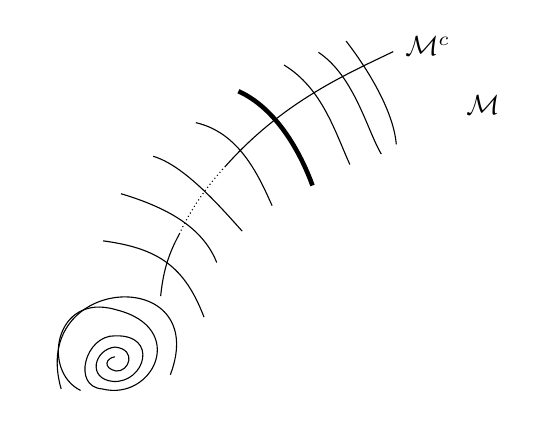
\begin{tikzpicture}[x=.95cm,y=.95cm]
\draw (1.49,1.36) .. controls (1.52,1.64) and (1.57,1.88) .. (1.74,2.19);
\draw[densely dotted] (1.74,2.19) .. controls (1.89,2.52) and (2.10,2.82) .. (2.35,3.09);
\draw (2.35,3.09) .. controls (3.12,3.96) and (3.98,4.33) .. (4.60,4.63);
\draw (.72,2.10) .. controls (1.46,2.00) and (1.81,1.76) .. (2.07,1.08);
\draw (.96,2.73) .. controls (1.56,2.55) and (2.05,2.29) .. (2.24,1.81);
\draw (1.39,3.23) .. controls (1.81,3.11) and (2.31,2.53) .. (2.58,2.23);
\draw (1.96,3.68) .. controls (2.53,3.55) and (2.79,3.00) .. (2.98,2.57);
\draw[line width=1.65pt] (2.53,4.10) .. controls (3.04,3.87) and (3.36,3.28) .. (3.52,2.84);
\draw (3.14,4.45) .. controls (3.65,4.14) and (3.82,3.56) .. (4.02,3.12);
\draw (3.60,4.62) .. controls (4.08,4.30) and (4.25,3.58) .. (4.44,3.26);
\draw (3.97,4.77) .. controls (4.31,4.33) and (4.61,3.79) .. (4.64,3.39);
\node[anchor=west] at (4.63,4.70) {\(\mathcal M^c\)};
\node at (5.80,3.92) {\(\mathcal M\)};
\draw (0.16,.12) .. controls (-.28,1.66) and (2.18,1.79) .. (1.62,.31);
\draw (0.42,.10) .. controls (-.11,.36) and (.08,1.42) .. (.89,1.18)
 .. controls (1.87,.94) and (1.39,-.05) .. (.71,.12)
 .. controls (.30,.15) and (.48,.84) .. (.88,.83)
 .. controls (1.47,.85) and (1.28,.20) .. (.86,.22)
 .. controls (.50,.25) and (.60,.65) .. (.88,.68)
 .. controls (1.18,.65) and (1.07,.34) .. (.89,.36)
 .. controls (.72,.40) and (.75,.53) .. (.88,.55);
\end{tikzpicture}}\endgroup}\par\smallskip
The lower part of the sloping line is faint. The joins at the spiral are indistinct.}
\end{GelfandAdjacentEvidence}


F.-P. trick

\(\nu\) --- the factor (at the integral over the orbits), which will be written out below.

There are two invariant metrics on the orbit; a) restriction of the metric of \(\mathcal M\): \(dg\)

b) [its own natural metric (transferred from the group --- the induced measure on \(G/H\), \(H\)---the stabilizer subgroup)]

\(\nu\) --- the ratio of the two measures on each orbit.


\Needspace{7\baselineskip}
\begin{GelfandAdjacentEvidence}{GELFAND-P001215}{1}
\SourcePage{GELFAND-P001215}{unlabelled}
\(\delta g\) --- variation of the metric --- tangent vector to the space of metrics.
\begin{equation*}
\begin{aligned}
|\delta g|^2
&=\int_{\mathcal E}(\delta g,\delta g)\,\text{vol. form}
=\int_{\mathcal E}(\delta g,\delta g)\omega\\
&=\int_{\mathcal E}(\delta g,\delta g)\sqrt g\,d\xi_1\,d\xi_2
\end{aligned}\tag{8}
\end{equation*}
\begin{equation*}
\mathcal Dg\text{ --- the volume form [inserted: on }\mathcal M\text{], corresponding to }|\delta g|^2\tag{9}
\end{equation*}
([overwritten mark] volume form constructed from the metric)
\Unclear{GELFAND-P001215}{volume-overwrite}{The overwritten mark before “volume form” may be an opening quotation mark or \(=\).}
\end{GelfandAdjacentEvidence}
\begin{GelfandAdjacentEvidence}{GELFAND-P001215}{2}


\(L\) --- the Lie algebra of the diffeomorphism group, i.e. the Lie algebra of vector fields on \(\mathcal E\).

\(\varepsilon\in L\)
\begin{equation*}
|\varepsilon|^2=\int_{\mathcal E}(\varepsilon,\varepsilon)\,\text{vol. form}
=\int_{\mathcal E}(\varepsilon,\varepsilon)\sqrt g\,d\xi_1\,d\xi_2\tag{10}
\end{equation*}
\begin{equation*}
\delta_\varepsilon g\in S^2(T^*)\tag{11}
\end{equation*}
\textit{[At right:]} (variation of the metric in the direction \(\varepsilon\)).

\textit{[Below the expression:]} --- Lie derivative.
\Unclear{GELFAND-P001215}{lie-derivative-cancelled}{The crossed-out words below \(\delta_\varepsilon g\) may read “vector fields.”}
\end{GelfandAdjacentEvidence}
\begin{GelfandAdjacentEvidence}{GELFAND-P001215}{3}


define the operator:
\begin{equation*}
L=\Gamma(T)\overset{D}{\longrightarrow}\Gamma(S^2(T^*)),
\qquad D(\varepsilon)=\delta_\varepsilon g\tag{12}
\end{equation*}
\textit{[Below \(\Gamma(T)\):]} (vector fields). (\(g\) is fixed).
\Unclear{GELFAND-P001215}{tensor-power-overwrite}{The overwritten exponent on \(S\) on the right of (12) has the visible form of \(2\). The earlier sign is illegible.}
\end{GelfandAdjacentEvidence}
\begin{GelfandAdjacentEvidence}{GELFAND-P001215}{4}

\begin{equation*}
\begin{aligned}
\|\varepsilon\|^2
&=\int_{\mathcal E}(D\varepsilon,D\varepsilon)\,\text{vol. form}\\
&=\int_{\mathcal E}(D\varepsilon,D\varepsilon)\sqrt g\,d\xi_1\,d\xi_2
\end{aligned}\tag{13}
\end{equation*}
\begin{equation*}
\frac{\text{vol. form corresponding to }\|\quad\|}{\text{vol. form corresponding to }\lvert\quad\rvert}
=(\det\Delta)^{1/2},\qquad\text{where }\Delta=D^*D\tag{14}
\end{equation*}
\textit{[In the right margin, beyond the double line:]} \(\Delta\) --- Laplace operator on vector fields;
\(\Delta:\Gamma(T)\to\Gamma(T)\).

The ratio (14) is by definition the factor \(\nu\) in (7)
\[
\Gamma(S^2T)\subset\Gamma(\operatorname{Hom}(T,T))
\]
\textit{[Below \(\operatorname{Hom}(T,T)\), brace:]} scalars \(\oplus\) trace 0.

\textit{[At right:]} (because of the metric); (identify \(S^2T\), \(S^2T^*\) and embed in \(\operatorname{Hom}(T,T)\)).

Corresponding decompositions of the sections:
\begin{equation*}
\Gamma(S^2T)=\Gamma(S^2T)^c\oplus\Gamma(S^2T)^{\mathrm{diff}}\tag{15}
\end{equation*}
\textit{[Below the first summand:]} conformal changes of the metric.

\textit{[Below the second summand:]} changes under the action of Lie derivatives.

[crossed out]
\begin{equation*}
(S^2T)^{\mathrm{diff}}=T\otimes\Omega^{0,1}\tag{16}
\end{equation*}
\Unclear{GELFAND-P001215}{eq16-cancelled}{A mark before the left side of (16) is crossed out, possibly \(\Gamma\) or \(\Phi\).}
\end{GelfandAdjacentEvidence}
\begin{GelfandAdjacentEvidence}{GELFAND-P001215}{5}

\Unclear{GELFAND-P001215}{bundle-splitting}{The superscript in (16) reads “diff.” Its precise role in the equality is unspecified.}
\end{GelfandAdjacentEvidence}
\begin{GelfandAdjacentEvidence}{GELFAND-P001215}{6}


[crossed out] It turns out that
\begin{equation*}
D=\bar\partial:\Gamma(T)\longrightarrow\Gamma(T\otimes\Omega^{0,1})\tag{17}
\end{equation*}
\Unclear{GELFAND-P001215}{before-eq17-cancelled}{An undeciphered mark before “It turns out that” is crossed out.}
\end{GelfandAdjacentEvidence}


[The metric determines on \(\mathcal E\) a complex structure, so it makes sense to write \(\Omega^{0,1}\)]
\[
(S^2T)^{\mathrm{diff}}\sim\text{-matrix }\begin{pmatrix}a&b\\b&-a\end{pmatrix};
\]
the meaning of (16) --- the matrix is determined by its first row.

\(T\) --- a holomorphic bundle, \(\Omega^{0,1}\) --- a 1-dimensional complex bundle.

\underline{on \(T\) acts} the group of rotations.

\(S^2T\) --- a 3-dimensional bundle, decompose it under the action of the rotation group.


\Needspace{7\baselineskip}
\begin{GelfandAdjacentEvidence}{GELFAND-P001216}{1}
\SourcePage{GELFAND-P001216}{80}
\uwave{Explanation of formula} (14):

[\(\Delta\) --- the operator corresponding to quadratic form (13) relative to quadratic form (10);].

Incidentally:

\(\delta_\varepsilon g\) --- the Lie derivative of the metric \(g\) in the direction \(\varepsilon\).

[A second way to define \(\Delta\) on \(\Gamma(T)\): identify \(T\) and \(T^*\)
using the metric and take \(\Delta\) on 1-forms.
We get the same thing, since \(d\) (de Rham differential) and the Lie derivative are dual to one another].
\Unclear{GELFAND-P001216}{duality-statement}{The last line in brackets reads “and the Lie derivative are dual to one another.” The note specifies no pairing.}
\end{GelfandAdjacentEvidence}


\(S^2T=S^2T^*\) in the presence of the metric.


\Needspace{7\baselineskip}
\begin{GelfandAdjacentEvidence}{GELFAND-P001217}{1}
\SourcePage{GELFAND-P001217}{unlabelled}
\underline{\underline{21/X--85.}}\qquad \uwave{Gelfand Seminar.}

\underline{\underline{Ryzhikova}} (A. Semenov’s student, in her 5th year).

\uwave{An algorithm for checking any identity in the structure of subspaces} [crossed out] \uwave{of a finite-dimensional space}.
\Incomplete{GELFAND-P001217}{struck-prefix}{The crossed-out parenthesis before “finite-dimensional space” is undeciphered.}
\end{GelfandAdjacentEvidence}
\begin{GelfandAdjacentEvidence}{GELFAND-P001217}{2}


We see which dimension suffices for checking [crossed out]
\Unclear{GELFAND-P001217}{dimension-final-mark}{The crossed-out mark after “checking” may be \(2\) or a question mark.}
\end{GelfandAdjacentEvidence}
\begin{GelfandAdjacentEvidence}{GELFAND-P001217}{3}

\[
a(ab+c)=ab+ac\qquad\text{or}\qquad
a(b+c)=ab+ac\quad\text{when }b\leq a
\]
\textit{[Below:]} dimension 2 suffices.

General formula: it is enough to check in a space of dimension
\[
n=\min[\max(d(p),d(q)),\max(k(p),k(q))]+1
\]
\(p,q\) --- 2 given terms

\(d(p)\) --- the number of additions in \(p\) (disjunction)

\(k(p)\) --- ″ --- multiplications in \(p\) (conjunction)

In a space of fixed dimension (over \(\mathbb R\)) there is Tarski’s algorithm.

\Needspace{6\baselineskip}
\underline{\underline{Fuchs}} (following Feigin). \underline{Continuation} \uwave{on strings}.

We need to evaluate the integral:
\begin{equation*}
\int_{\mathcal M^c}(\operatorname{Det}\Delta)^{-d/2}\nu\tag{1}
\end{equation*}
\underline{Feigin.}

We need to compute the integral
\begin{equation*}
\int_{\mathcal M_t}(\operatorname{Det}\Delta_0)^{-d/2}\mathcal Dg
=\int_{\mathcal M_t^c}\frac{\operatorname{Det}\Delta_1}{(\operatorname{Det}\Delta_0)^{d/2}}\mathcal Dg,\tag{2}
\end{equation*}
\Unclear{GELFAND-P001217}{eq2-domain-cancelled}{In (2) the superscript on \(\mathcal M_t\) under the first integral is crossed out, possibly \(c\).}
\end{GelfandAdjacentEvidence}
\begin{GelfandAdjacentEvidence}{GELFAND-P001217}{4}

\Unclear{GELFAND-P001217}{eq2-cancelled-formula}{The writing to the right of (2) is crossed out, possibly \(\Delta=\Delta_0\) or \(\Delta\ne\Delta_0\).}
\end{GelfandAdjacentEvidence}
\begin{GelfandAdjacentEvidence}{GELFAND-P001217}{5}

\EvidenceBlock{GELFAND-P001217}{eq2-determinant-power}{The numerator is written \(\operatorname{Det}\Delta_1\) with no exponent. The denominator carries exponent \(d/2\).}{}
\end{GelfandAdjacentEvidence}


\(\mathcal M\) --- the space of metrics, \(t\) --- a point in the moduli space of curves of genus \(g\)

\(\mathcal M_t\) --- the space of metrics for the complex structure corresponding to modulus \(t\).


\Needspace{7\baselineskip}
\begin{GelfandAdjacentEvidence}{GELFAND-P001218}{1}
\SourcePage{GELFAND-P001218}{87}
\(\mathcal M_t^c\) --- the set of metrics [inserted above the line: (corresponding to the given modulus \(t\))] of the form \(e^\varphi g_0\),
where \(g_0\) --- a metric of constant negative curvature \(=-1\).
\Unclear{GELFAND-P001218}{upper-margin-abbreviation}{The note below \(\mathcal M_t^c\) reads “na pv., sootv. \(t\).” A possible expansion is “on the surface corresponding to \(t\).”}
\end{GelfandAdjacentEvidence}
\begin{GelfandAdjacentEvidence}{GELFAND-P001218}{2}


\(T\) --- the tangent bundle on the curve (already equipped with a complex structure)
\[
\bar\partial:\Gamma(T^j)\longrightarrow\Gamma(T^j\otimes\Omega^{0,1}),
\qquad\Delta_j=\bar\partial^*\bar\partial
\]
\Unclear{GELFAND-P001218}{gamma-cancelled-parenthesis}{After \(T^j\) and before \(\otimes\), the upper arc of a crossed-out mark is visible, probably a closing parenthesis.}
\end{GelfandAdjacentEvidence}
\begin{GelfandAdjacentEvidence}{GELFAND-P001218}{3}


In fact \(\mathcal M_t^c\) [crossed out]; \(\mathcal M_t^c\subset\mathcal M_t\)
[crossed out]
\Unclear{GELFAND-P001218}{mt-cancelled-mark}{An undeciphered mark after the first \(\mathcal M_t^c\) is crossed out.}
\end{GelfandAdjacentEvidence}
\begin{GelfandAdjacentEvidence}{GELFAND-P001218}{4}

\Unclear{GELFAND-P001218}{mt-cancelled-inclusion}{At right, the crossed-out expression may be \((\mathcal M^c\subset\mathcal M_t)\) or \((\mathcal M_t^c\subset\mathcal M_t)\).}
\end{GelfandAdjacentEvidence}
\begin{GelfandAdjacentEvidence}{GELFAND-P001218}{5}


(\(t\) is fixed).

Every metric in \(\mathcal M_t\) can be (by the action of \(\operatorname{Diff}\))
\EvidenceBlock{GELFAND-P001218}{unfinished-sentence}{The sentence stops after “(by the action of Diff).”}{}
\end{GelfandAdjacentEvidence}
\begin{GelfandAdjacentEvidence}{GELFAND-P001218}{6}


The moduli space has dimension \(\underline{3g-3}\).

The integral over it has yet to be evaluated (much work is devoted to it).

\Incomplete{GELFAND-P001218}{mid-cancelled-formula}{The short crossed-out formula before the line about \(\operatorname{Det}\Delta_0\) is undeciphered.}
\end{GelfandAdjacentEvidence}
\begin{GelfandAdjacentEvidence}{GELFAND-P001218}{7}


\(\operatorname{Det}\Delta_0\) --- is taken over the nonzero eigenvalues.

\(\operatorname{Det}\Delta_j=\operatorname{Det}\Delta_j(\varphi)\).

Next,
\begin{equation*}
\begin{aligned}
\delta\ln\operatorname{Det}\Delta_j(\varphi)
&=(Aj+B)\int_{\mathcal E}\delta\varphi\cdot\operatorname{Vol}\\
&\quad+C(6j^2+6j+1)\int_{\mathcal E}\delta\varphi\cdot K\cdot\operatorname{Vol}
\end{aligned}\tag{3}
\end{equation*}
\Unclear{GELFAND-P001218}{eq3-coefficient}{The original coefficient is crossed out. The insertion reads \((Aj+B)\), possibly \((A_j+B)\).}
\end{GelfandAdjacentEvidence}
\begin{GelfandAdjacentEvidence}{GELFAND-P001218}{8}

\EvidenceBlock{GELFAND-P001218}{eq3-denominator-cancelled}{The fraction bar and the denominator \(\delta\varphi\) below the left-hand side are crossed out.}{}
\end{GelfandAdjacentEvidence}
\begin{GelfandAdjacentEvidence}{GELFAND-P001218}{9}


\textit{[Below the first \(\operatorname{Vol}\), brace:]} volume form.

(\(j\) --- “spin”)

\(A,B,C\) --- some constants; \(K\) --- the Gaussian curvature of the surface.
\[
\begin{aligned}
j=1&\Rightarrow 6j^2+6j+1=13\\
j=0&\Rightarrow 6j^2+6j+1=1
\end{aligned}
\]
\Unclear{GELFAND-P001218}{j-zero-value-overwritten}{The overwritten result on the \(j=0\) line has the visible form of \(1\). The earlier writing is illegible.}
\end{GelfandAdjacentEvidence}
\begin{GelfandAdjacentEvidence}{GELFAND-P001218}{10}


At \(d=26\) the anomaly cancels.

And then one has to integrate a constant (on the right-hand side of (2))

\underline{Corollary}:
\begin{equation*}
\ln\operatorname{Det}\Delta_j(\varphi)
=A\int\text{[crossed out]}\,\varphi\cdot\partial\bar\partial\varphi
+B\int e^\varphi\operatorname{Vol}
+C\int\varphi\operatorname{Vol}+D\tag{4}
\end{equation*}
\Unclear{GELFAND-P001218}{eq4-cancelled-term}{The crossed-out expression immediately after the first integral sign in (4) may read \(\partial\varphi\wedge\bar\partial\varphi\) or \(\partial\varphi\,\bar\partial\varphi\).}
\end{GelfandAdjacentEvidence}


(\(A,B,C,D\) --- constants)

\(\Rightarrow\) the calculation is equivalent to the Liouville equation (in (4) its Lagrangian)

Solving the Liouville equation is equivalent to computing
\begin{equation*}
\int e^{\mathcal L_j(\varphi)}\mathcal D\varphi,\tag{5}
\end{equation*}
where \(\mathcal L_j(\varphi)\) --- left (\(=\) right) side of (4)

\(\ln\operatorname{Det}\Delta_j\) is taken as the Lagrangian of the new theory. It is clear that
\begin{equation*}
(2)=\int e^{\mathcal L_1(\varphi)-\frac d2\mathcal L_0(\varphi)}\mathcal D\varphi.\tag{6}
\end{equation*}


\clearpage
\pdfbookmark[0]{Chapter 27}{gelfand-archive-chapter-27}
\section*{Chapter 27}
\Needspace{7\baselineskip}
\begin{GelfandAdjacentEvidence}{GELFAND-P001219}{1}
\SourcePage{GELFAND-P001219}{unlabelled}
\underline{\(28/\overline{\underline{X}}\)---85 }\qquad \underline{Gelfand Seminar}

\underline{W. Müller.}

\uwave{Cheeger / Gromov}

\(X\) --- a complete Riemannian manifold, \(\operatorname{vol}(X)<\infty\), \(\lvert K\rvert<1\).

\textit{[Below \(K\):]} sectional curvature.
\[
\int p(\Omega)\;-\;?
\]
\underline{Theorem.} \(X\) --- the interior of a compact manifold with boundary
\textit{[Below “interior”: (diffeomorphic)]}
\[
\Rightarrow 1)\;\int_X p(\Omega)=\chi(X).
\]
\Unclear{GELFAND-P001219}{formula-cancellation}{An undeciphered mark above \(p(\Omega)\) is crossed out.}
\end{GelfandAdjacentEvidence}



\Needspace{7\baselineskip}
\begin{GelfandAdjacentEvidence}{GELFAND-P001220}{1}
\SourcePage{GELFAND-P001220}{unlabelled}
\begin{equation*}
2)\quad \int_X L_k(p_1,\ldots,p_k)\quad\text{--- homotopy invariant}
\end{equation*}
Question related to the work of \underline{Cheeger}

mfd [inserted above the line \(X\)] with cone like singularity

\SourceFigure{GELFAND-P001220}{cone-sketch}{%
\par\smallskip
{\color{black}\begingroup\color{black}\GelfandFitDiagram{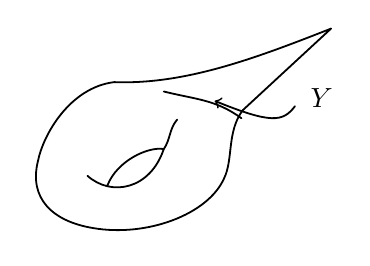
\begin{tikzpicture}[x=.17mm,y=.17mm,line width=.65pt,line cap=round,line join=round]
\draw (269,153) .. controls (213,131) and (160,111) .. (107,113)
 .. controls (74,109) and (54,74) .. (50,54)
 .. controls (43,26) and (61,9) .. (91,4)
 .. controls (131,-3) and (177,14) .. (189,41)
 .. controls (196,55) and (191,76) .. (203,92) -- cycle;
\draw (87,43) .. controls (105,27) and (134,33) .. (144,63)
 .. controls (132,65) and (109,54) .. (102,36);
\draw (144,63) .. controls (149,70) and (148,78) .. (154,85);
\draw (144,106) .. controls (168,100) and (183,100) .. (202,86);
\draw[->] (242,95) .. controls (233,83) and (224,82) .. (182,99);
\node at (262,101) {\(Y\)};
\end{tikzpicture}}\endgroup}\par\smallskip
The pointer strokes overlap at the neck.}
\end{GelfandAdjacentEvidence}
\begin{GelfandAdjacentEvidence}{GELFAND-P001220}{2}


\(\Delta\) on \(\Lambda^*\)

\(\Delta\) on cone
\begin{equation*}
-\frac{\partial^2}{\partial u^2}+u^{-2}A(u)
\end{equation*}
\begin{equation*}
A(u)\in L^2((0,1],\Lambda^*(Y))
\end{equation*}
\Unclear{GELFAND-P001220}{function-or-operator}{Both lines read \(A(u)\). The first has a membership sign and the second gives a map. The \(u\) on the second line is retraced. The role of \(A(u)\) across the two lines is unclear.}
\end{GelfandAdjacentEvidence}
\begin{GelfandAdjacentEvidence}{GELFAND-P001220}{3}

\begin{equation*}
\begin{gathered}
A(u):\Lambda^*(Y)\longrightarrow\Lambda^*(Y),\\
C(Y)=(0,1]\times Y,\\
ds^2=du^2+u^{-2}g_Y.
\end{gathered}
\end{equation*}
\EvidenceBlock{GELFAND-P001220}{cone-metric-exponent}{The exponent on \(u\) before \(g_Y\) is \(-2\).}{Manuscript notation.}
\end{GelfandAdjacentEvidence}

\begin{equation*}
\operatorname{Tr}(e^{-t\Delta})\underset{t\to0+}{\sim}
\sum_{j\geq0}a_jt^{-(n-j)/2}+c\log t+b
\end{equation*}
\begin{equation*}
b=b_0\zeta_Y(-1)+\sum_{j\geq1}b_j
\underset{s=2j-1}{\operatorname{Res}}\zeta_Y(s)
\end{equation*}
\begin{equation*}
\zeta_Y(s)=\sum_{\lambda_j}\lambda_j^{-s}
\end{equation*}
\begin{equation*}
D_s=d+\delta:\Lambda^*_+(X)\longrightarrow\Lambda^*_-(X)
\qquad\text{signature operator}
\end{equation*}
[Below:] signature operator
\begin{equation*}
(*)\qquad \operatorname{Ind}D_s=\int_X L_k(p_1,\ldots,p_k)+\eta_Y(B),
\qquad\text{where \(B\) is defined below.}
\end{equation*}
\(\dim X=4k\).

[Under the bracket at the integral] this would be the index without boundary.

[Enclosed by a bracket] \(L_k=0\) \uwave{on the cone}.

On the cone:
\begin{equation*}
d+\delta=D_s=-\frac{\partial}{\partial u}+u^{-1}B,
\qquad B:\Lambda^*(Y)\longrightarrow\Lambda^*(Y).
\end{equation*}
[At right, beyond the double vertical line] On \(\Lambda^{ev}\), \(B\) has the form \(\pm(*d-d*)\).
\begin{GelfandAdjacentEvidence}{GELFAND-P001220}{4}
\begin{equation*}
D=\frac{\partial^n}{\partial u^n}+\sum u^{i-n}\frac{\partial^i}{\partial u^i}A_j
\end{equation*}
\EvidenceBlock{GELFAND-P001220}{operator-indices}{The exponent on \(u\) and both orders in the derivative have \(i\). The coefficient has subscript \(j\). No limits are written on the sum.}{Manuscript notation.}
\end{GelfandAdjacentEvidence}


\(A_j\) --- diff. op. on \(Y\).

\uwave{index --- ?}

Cheeger's example gives \(\eta\)! --- formula \((*)\)


\Needspace{7\baselineskip}
\begin{GelfandAdjacentEvidence}{GELFAND-P001221}{1}
\SourcePage{GELFAND-P001221}{6}
The index is defined on fns. satisfying [crossed out] the condition at the singularity:
\Unclear{GELFAND-P001221}{top-cancellation}{The crossed-out word before “the condition” is illegible.}
\end{GelfandAdjacentEvidence}
\begin{GelfandAdjacentEvidence}{GELFAND-P001221}{2}

\begin{equation*}
\lim_{u\to0}u^{-1/2}\varphi(u)=\lim_{u\to0}u^{1/2}\varphi'(u)
\end{equation*}
\uwave{Relation to representations.}
\begin{equation*}
X=K\backslash G/\Gamma\qquad\text{loc symm.},\quad\operatorname{vol}(X)<\infty
\end{equation*}
\(\mathcal E,\mathcal F\longrightarrow X\)\quad loc. [crossed out]
[above the line: triv.\ (?)] vectorbundles
\Unclear{GELFAND-P001221}{bundle-correction}{“triv. (?)” appears above the crossing-out. The first stroke of the crossed-out abbreviation is consistent with “triv.”. The cancellation obscures the remaining letters.}
\end{GelfandAdjacentEvidence}
\begin{GelfandAdjacentEvidence}{GELFAND-P001221}{3}

\begin{equation*}
D:C_0^\infty(X,\mathcal E)\longrightarrow C_0^\infty(X,\mathcal F)
\qquad\text{oper. loc inv.}
\end{equation*}
\underline{Th.}
\begin{equation*}
\begin{gathered}
\ker\bar D<\infty,\\
\ker\bar D^*<\infty.
\end{gathered}
\end{equation*}
\begin{equation*}
\operatorname{Ind}_{L^2}D=\dim\ker\bar D-\dim\ker\bar D^*
\end{equation*}
\begin{center}\rule{.9em}{.35pt}\quad\rule{.9em}{.35pt}\end{center}
\begin{equation*}
X=H\times H/SL(2,O_F),\qquad F=Q(\sqrt D),\quad D>0.
\end{equation*}
\Unclear{GELFAND-P001221}{group-cancellation}{A mark before \(O_F\) in \(SL(2,O_F)\) is heavily crossed out.}
\end{GelfandAdjacentEvidence}
\begin{GelfandAdjacentEvidence}{GELFAND-P001221}{4}


only 1 cusp
\begin{equation*}
D_s=d+\delta:\Lambda^*_+(X)\longrightarrow\Lambda^*_-(X)
\end{equation*}
\begin{equation*}
\operatorname{ind}D_s=\frac13\int_X p_1-\frac1{2\pi}L(M,V,1)\operatorname{vol}(\mathbb R^2/M)
\end{equation*}
\Unclear{GELFAND-P001221}{integrand-mark}{The heavily inked mark after \(p_1\) and before the minus resembles \(A\) or \(\Delta\). Its cancellation status is unclear.}
\end{GelfandAdjacentEvidence}
\begin{GelfandAdjacentEvidence}{GELFAND-P001221}{5}

\begin{equation*}
M=O_F,\qquad V=O_F^{*2}
\end{equation*}
\begin{equation*}
L(M,V,s)=\sum_{\mu\in(M-0)N_F}\frac{\operatorname{sign}N(\mu)}{|N(\mu)|^s}
\end{equation*}
\EvidenceBlock{GELFAND-P001221}{sum-domain}{The symbols \(N_F\) follow the closing parenthesis directly below the sum sign.}{Manuscript notation.}
\end{GelfandAdjacentEvidence}
\begin{GelfandAdjacentEvidence}{GELFAND-P001221}{6}


\underline{\underline{Feigin.}}\qquad\uwave{On strings}\qquad(work of \underline{Polyakov})

(\underline{Continued.})

\(\mathcal E\) --- Riem. surface of genus \(g\)

\(T\) --- tangent bundle

On \(\mathcal E\) a complex structure induced by the Riem. metric is chosen, and the operator \(\bar\partial:T^j\longrightarrow T^j\otimes\Omega^{0,1}\);
\begin{equation*}
\Delta_j=\bar\partial^*\bar\partial
\end{equation*}
\begin{equation*}
0\longrightarrow H^0(T^j)\longrightarrow\Gamma(T^j)
\overset{\bar\partial}{\longrightarrow}\Gamma(T^j\otimes\Omega^{0,1})
\longrightarrow H^1(T)\longrightarrow0.\tag{1}
\end{equation*}
\EvidenceBlock{GELFAND-P001221}{sequence-final-term}{The term before zero in (1) is \(H^1(T)\). There is no exponent on \(T\).}{Manuscript notation.}
\end{GelfandAdjacentEvidence}



\Needspace{7\baselineskip}
\begin{GelfandAdjacentEvidence}{GELFAND-P001222}{1}
\SourcePage{GELFAND-P001222}{unlabelled}
The problem can be reformulated as computing the Ray--Singer torsion of this complex.
\begin{equation*}
g_{ij}\longrightarrow g_{ij}(1+\varepsilon\rho)\tag{2}
\end{equation*}
\(\bar\partial\) has \(\ker\) and \(\operatorname{coker}\).
[In the same interlinear note:] What was actually computed was the change

in Ray--Singer torsion [crossed out] of the complex (1) under deformation
\Unclear{GELFAND-P001222}{torsion-cancellation}{The rightmost sign in the crossed-out notation after “Singer” resembles \(\bar\partial\). The middle may read \(\operatorname{Det}\).}
\end{GelfandAdjacentEvidence}
\begin{GelfandAdjacentEvidence}{GELFAND-P001222}{2}


on \(\Gamma(T^j)\) and on \(\Gamma(T^j\otimes\Omega^{0,1})\)
there are Hermitian metrics.

They induce Herm. metrics on \(\underbrace{H^0(T^j)}_{\text{subspace}}\) and \(H^1(T^j)\).

\(\ker\bar\partial\bar\partial^*\) is identified with \(H^1(T^j)\)
\(\Rightarrow\) on \(H^1(T^j)\) there is a Herm. metric.
\begin{equation*}
\operatorname{Det}T^j:=\Lambda^{\max}H^0(T^j)
\otimes\bigl(\Lambda^{\max}H^1(T^j)\bigr)^*\tag{3}
\end{equation*}
(Quillen's terminol.)\qquad(1-dimensional space)

(4) On \(\operatorname{Det}T^j\) there is also a Hermitian metric. Denote it by \(\varepsilon\).

Ray--Singer torsion is another Herm. metric on \(\operatorname{Det}T^j\). It equals the Herm. metric (4) divided by \(\operatorname{Det}\Delta_j\):
\begin{equation*}
\frac{\varepsilon}{\operatorname{Det}\Delta_j}\tag{5}
\end{equation*}
Consider the variation of the metric:
\begin{equation*}
g_{ij}\longrightarrow g_{ij}(1+\varepsilon\rho)\tag{6}
\end{equation*}
Given a seq. of numbers \(j_1,j_2,\ldots,j_n\),
[inserted above the line: \(k_1,\ldots,k_n\)] and 1-dimensional space
\begin{equation*}
\operatorname{Det}(T^{j_1})^{k_1}\otimes
\operatorname{Det}(T^{j_2})^{k_2}\otimes\cdots\otimes
\operatorname{Det}(T^{j_n})^{k_n}\tag{7}
\end{equation*}
with Herm. metric \(=\) the product of the Ray--Singer torsions of each of these spaces.

(8) \underline{Claim.} The metric on (7) is unchanged under variation (6) if
\begin{equation*}
\sum_\alpha(6j_\alpha^2+6j_\alpha+1)k_\alpha=0.\tag{9}
\end{equation*}
\Unclear{GELFAND-P001222}{anomaly-extra-stroke}{A separate heavy diagonal stroke lies between \(\sum_\alpha\) and the opening parenthesis. The first \(6\) is retraced. The role of the separate stroke is unclear.}
\end{GelfandAdjacentEvidence}
\begin{GelfandAdjacentEvidence}{GELFAND-P001222}{3}


\uwave{Or:} under condition (9) the metric on (7) depends only on the complex structure.

Let \(\mathcal M\) --- moduli manifold of complex curves of genus \(g\).

The collection of spaces is a 1-dimensional bundle over \(\mathcal M\).

A metric is constr. on this bundle (a similar constr. occurs in [Fal'tingsa?])
\Unclear{GELFAND-P001222}{final-name}{The surname at the end of the line tentatively reads «Фальтингса» (Fal'tingsa). The joined final strokes also allow «Фальтинга» (Fal'tinga).}
\end{GelfandAdjacentEvidence}



\Needspace{7\baselineskip}
\begin{GelfandAdjacentEvidence}{GELFAND-P001223}{1}
\SourcePage{GELFAND-P001223}{unlabelled}
\(4/\overline{\underline{\mathrm{XI}}}-85\)\quad\underline{Gelfand Sem.}

\underline{\underline{Ryzhikova}}\quad\underline{On lattice representations.}
(work of Gelfand and Ponomarev)

\underline{Def.} An elem. \(a\in L\) is called \uwave{perfect}, if

(\(L\) --- a lattice)
\begin{equation*}
\begin{gathered}
\forall k,\quad\forall\rho:L\longrightarrow\mathcal L(V),\quad\exists U\subseteq V,\\
U+\rho(a)=V,\qquad U\rho(a)=0,\\
\forall x:\quad\rho(x)=\rho(a)\rho(x)+U\rho(x).
\end{gathered}
\end{equation*}
[Above \(k\) --- field. Above \(\rho\) --- rep..]

Or: \(\forall\) indecomposable rep., \(a\) maps to \(0\) or to the whole space.
\Unclear{GELFAND-P001223}{perfect-element-overwrite}{The overwritten sign before “maps” reads lowercase \(a\). The earlier strokes are indistinct.}
\end{GelfandAdjacentEvidence}
\begin{GelfandAdjacentEvidence}{GELFAND-P001223}{2}


\underline{Def. of a lattice.}

\(a+b\), \(a\cdot b\) --- assoc. commut.
\begin{equation*}
\begin{gathered}
a\cdot a=a,\qquad a+a=a,\qquad a(a+b)=a,\qquad a+ab=a,\\
a\leq b\Longleftrightarrow ab=a\Longleftrightarrow a+b=b,\\
a\leq b\Longrightarrow b(a+c)=a+bc.
\end{gathered}
\end{equation*}
Rep. of a lattice \(\rho:L\longrightarrow\mathcal L(V)\).

\begin{center}\rule{.9em}{.35pt}\quad\rule{.9em}{.35pt}\end{center}

[Crossed out: Consider.] [Above the line: Let us construct.] a countable number of cubes \(B^+(\ell)\) and \(B^-(\ell)\),
\(\ell\geq1\),
\EvidenceBlock{GELFAND-P001223}{construct-verb-correction}{«Построим» (Let us construct) appears above the crossed-out «Рассмотрим» (Consider).}{Manuscript notation.}
\end{GelfandAdjacentEvidence}


\(D^r\) --- free modular lattice with \(r\) generators \(e_1,\ldots,e_r\).


\Needspace{7\baselineskip}
\begin{GelfandAdjacentEvidence}{GELFAND-P001224}{1}
\SourcePage{GELFAND-P001224}{unlabelled}
1.\ \underline{\(\ell=1\)}

Put \(h_t(1)=\displaystyle\sum_{j\ne t}e_j\), \(t=1,\ldots,r\).

These \(h_t(1)\) [inserted above the crossing-out: generate] the Boolean algebra
\(B^+(1)\) [crossed out]
\Unclear{GELFAND-P001224}{upper-cancellation}{The crossed-out text after \(B^+(1)\) may begin with «уже» (uzhe). The remaining text is illegible.}
\end{GelfandAdjacentEvidence}
\begin{GelfandAdjacentEvidence}{GELFAND-P001224}{2}

\begin{equation*}
\begin{gathered}
0,\ h_1,\ldots,h_4,\quad h_1\cdot h_2,\ h_2\cdot h_3,\\
h_1\cdot h_2\cdot h_3,\ldots,\\
h_1\cdot h_2\cdot h_3\cdot h_4.
\end{gathered}
\end{equation*}
The sum of products is already expr. as a product.

2.\ \uwave{\(\ell=2\)}
\begin{equation*}
\{(i_1,i_2):i_1\ne i_2\}=A(r,2)
\end{equation*}
\begin{equation*}
\{(i_1,t),\ i_1\ne t\}=A_t(r,2)\qquad(t\text{ --- fixed})
\end{equation*}
\begin{equation*}
e_t(2)=\sum_{i_1=1}^{r}e_{i_1t}
=\sum e_{i_1}\left(\sum_{k\ne i_2,t}e_k\right)
\end{equation*}
\EvidenceBlock{GELFAND-P001224}{second-level-sum}{The limits of the first sum are \(i_1=1\) and \(r\). The inner sum has \(k\ne i_2,t\).}{Manuscript notation.}
\end{GelfandAdjacentEvidence}
\begin{GelfandAdjacentEvidence}{GELFAND-P001224}{3}

\begin{equation*}
h_t(2)=\sum_{j\ne t}e_j(2)
\end{equation*}
\begin{center}\rule{.9em}{.35pt}\quad\rule{.9em}{.35pt}\end{center}
\begin{equation*}
\{(i_1,\ldots,i_\ell),\ i_j\ne i_{j+1}\}=A(r,\ell)
\end{equation*}
\begin{equation*}
\{(i_1,\ldots,i_{\ell-1},t),\ i_{\ell-1}\ne t\}\cap A(r,\ell)=A_t(r,\ell)
\end{equation*}
\begin{equation*}
\Gamma(i_1,\ldots,i_\ell)=\{\beta=(k_1,\ldots,k_{\ell-1})\mid k_j\notin\{j_{i-1},j_i\}
\end{equation*}
\Unclear{GELFAND-P001224}{gamma-index}{The initial sign is provisionally read as \(\Gamma\). A reading of \(\Pi\) is possible. The last two subscripted letters resemble \(j\). The subscripts appear to read \(i-1\) and \(i\). One closing brace is visible.}
\end{GelfandAdjacentEvidence}
\begin{GelfandAdjacentEvidence}{GELFAND-P001224}{4}


These are all cubes (consisting of \(2^n\) elem.) --- Boolean algebras;
the lower ones are constructed dually.
\EvidenceBlock{GELFAND-P001224}{cardinality-exponent}{The exponent on \(2\) is \(n\).}{Manuscript notation.}
\end{GelfandAdjacentEvidence}
\begin{GelfandAdjacentEvidence}{GELFAND-P001224}{5}


They are all ordered.

\underline{Def.} \(V\) over \(K\) [inked over] of char. \(0\)
\Unclear{GELFAND-P001224}{char-cancellation}{There is a heavily inked mark between \(K\) and “of char.”.}
\end{GelfandAdjacentEvidence}


\(\rho:L\longrightarrow\mathcal L(V,K)\) is called completely irreducible if
\begin{equation*}
\rho(L)\cong\mathcal L(\mathbb Q^n)\cong P(n-1,\mathbb Q).
\end{equation*}


\Needspace{7\baselineskip}
\begin{GelfandAdjacentEvidence}{GELFAND-P001225}{1}
\SourcePage{GELFAND-P001225}{10}
\underline{\underline{B. L. Feigin}}\qquad\underline{On strings}

\underline{How do the Virasoro alg. and hypergeometric fns. arise?}

\uwave{Virasoro algebra}: Lie alg. \(\mathcal L\) with basis
\(\{e_i\}\), \(\underline{\underline{C}}\), \(i\in Z\).
\begin{equation*}
\begin{gathered}
\relax [e_i,e_j]=(j-i)e_{i+j}+\delta_{i,-j}\frac{i^3-i}{12}\underline{\underline{C}},\\[0pt]
[e_i,\underline{\underline{C}}]=0.
\end{gathered}\tag{1}
\end{equation*}
(2) Quotient by the center \(=\) alg. of vector fields on the circle.

For Verma modules see the book of \uwave{Dixmier} on enveloping algebras.

and 2 papers by Bernstein, [crossed out] I. M. G. and S. I. Gelfand in FA
\Unclear{GELFAND-P001225}{author-initials}{The crossed-out letter before “I. M. G.” may read «И» (I) or «Н» (N).}
\end{GelfandAdjacentEvidence}
\begin{GelfandAdjacentEvidence}{GELFAND-P001225}{2}


(including on categories «Оре»)
\Unclear{GELFAND-P001225}{category-reading}{The word after “categories” reads «Оре» (Ore). Its referent is unclear.}
\end{GelfandAdjacentEvidence}
\begin{GelfandAdjacentEvidence}{GELFAND-P001225}{3}

\begin{equation*}
\begin{gathered}
\mathfrak h=\{e_0,\underline{\underline{C}}\}\qquad(\text{Cartan}),\\
\mathcal L_+=\{e_1,e_2,e_3,\ldots\}\qquad(\text{creat.}),\\
\mathcal L_-=\{e_{-1},e_{-2},\ldots\}\qquad(\text{annih.}).
\end{gathered}
\end{equation*}
\(\chi=(h,\bar{\bar{c}})\) --- [crossed out] pair of numbers
\Unclear{GELFAND-P001225}{pair-cancellation}{The crossed-out abbreviation before “pair” may read «упор.» (upor.). Its expansion is unclear.}
\end{GelfandAdjacentEvidence}


Verma module: \(M_\chi\), there is a vac. vector \(v\)
\begin{equation*}
\begin{cases}
e_0v=hv,\\
Cv=\bar{\bar{c}}\,v
\end{cases}
\qquad\mathcal L_-v=0.\tag{3}
\end{equation*}
Physicists write \(L_i\) in place of \(e_i\).

(4) Given \(M_\chi=M_{h,c}\), \uwave{when is} [inserted above the line: it]
\uwave{reducible}?

\begin{GelfandAdjacentEvidence}{GELFAND-P001225}{4}
Physicists call these \uwave{mass formulas} (mass spectrum)
\begin{equation*}
\begin{aligned}
0=\Phi_{k_1k_2}(h,c)
&=\prod_{j=1,2}\left\{h+\frac{c-13}{24}(k_j^2-1)+\frac12(k_1k_2-1)\right\}+\\
&\quad+\frac12(k_1^2-k_2^2)^2.
\end{aligned}\tag{5}
\end{equation*}
\EvidenceBlock{GELFAND-P001225}{kac-coefficient}{The coefficient of \((k_1^2-k_2^2)^2\) in (5) is \(1/2\). A plus is written at the end of the preceding line and before the fraction.}{Manuscript notation.}
\end{GelfandAdjacentEvidence}


(Kac formula)

Here \(k_1,k_2\) --- natural numbers.

(6) \underline{Claim.} [Below the heading: (Feigin, Fuchs).]
If \(\exists\) \(k_1,k_2\), satisfying (5), the rep. is reducible. If none exist, it is irreducible.

(7) \underline{Addendum}: if \(M_\chi\) is reducible, in it
\(\exists\) a vector different from the vac. vector and annihilated by all annih. operators (a “singular vector”).

\(\mathcal L\) is naturally graded \(\Rightarrow M_\chi\) is too.


\Needspace{7\baselineskip}
\begin{GelfandAdjacentEvidence}{GELFAND-P001226}{1}
\SourcePage{GELFAND-P001226}{unlabelled}
(8) Then the level of the sing. vector \(=k_1\cdot k_2\).

\uwave{Proofs:} constructions of various beautiful reps. \uwave{of 2 types}.
\Unclear{GELFAND-P001226}{type-count}{The final form of the overwritten numeral before “types” reads \(2\). The earlier strokes are indistinct.}
\end{GelfandAdjacentEvidence}
\begin{GelfandAdjacentEvidence}{GELFAND-P001226}{2}


\uwave{1st type.}
\begin{equation*}
\mathcal L/C\longrightarrow gl_\infty,\ O_\infty,\ sp_\infty
\end{equation*}
[Below the quotient: (v. fields).]
\Unclear{GELFAND-P001226}{quotient-centre}{The overwritten sign after the slash is provisionally read as \(C\). The case is unclear and \(c\) is possible.}
\end{GelfandAdjacentEvidence}
\begin{GelfandAdjacentEvidence}{GELFAND-P001226}{3}


\uwave{2nd type}

(9) \(\mathcal L\hookrightarrow\) the enveloping alg. of an affine Kac--Moody algebra.

We construct the embedding

\(\mathfrak g\) --- finite-dim. simple Lie alg.

\(\widehat{\mathfrak g}\) --- 1-dimensional extension of the current algebra (usually called a Kac--Moody alg.)

[Between the lines:] ([crossed out] \uwave{I.M.G.} Current alg. --- alg. of matrix fns. on the circle).
\Unclear{GELFAND-P001226}{current-comment-cancellation}{The crossed-out mark before “I.M.G.” is illegible.}
\end{GelfandAdjacentEvidence}
\begin{GelfandAdjacentEvidence}{GELFAND-P001226}{4}


On \(\mathfrak g\) fix the Killing form.

(10) Choose \(u_\alpha\in\mathfrak g_\alpha\) (root space) so that
\((u_\alpha,u_{-\alpha})=1\).

(11) Choose \(u_1,\ldots,u_\ell\in\mathfrak h\), \(u^1,\ldots,u^\ell\) --- dual basis.

[Under \(u_1,\ldots,u_\ell\): (basis).]

Put
\begin{equation*}
\begin{aligned}
S(m)&=\sum_{j=1}^{\ell}\sum_{r\in Z}:u^j(-r)u_j(r+m):+\\
&\quad+\sum_{\alpha\in\Delta}\sum_{r\in\Delta}:u_{-\alpha}(-r)u_\alpha(r+m):
\end{aligned}\tag{12}
\end{equation*}
(elements of the enveloping alg.)
\EvidenceBlock{GELFAND-P001226}{root-sum-domain}{The inner sum on the first line of (12) has \(r\in Z\). The inner sum on the second line has \(r\in\Delta\).}{Manuscript notation.}
\end{GelfandAdjacentEvidence}


The order \({:}\quad{:}\) always in \(u(r)u(s)\) is set so that
\(r<s\) or if \(r=s\), we replace the product by the half-sum of the products.

\(S(m)\) are called Graeme Segal operators.
\begin{equation*}
\begin{aligned}
\relax [S(m),S(n)]&=2(n-m)\cdot(g+k)S(m+n)+\\
&\quad+\frac{\dim\mathfrak g}{12}\delta_{m,-n}(m^3-m)4(g+k)k.
\end{aligned}\tag{13}
\end{equation*}
(\(k\) --- a number)

\(S(m)\) act in a representation of the alg. \(\widehat{\mathfrak g}\), in which the center acts by multiplication by \(k\) (for example, in a Verma module).


\Needspace{7\baselineskip}
\begin{GelfandAdjacentEvidence}{GELFAND-P001227}{1}
\SourcePage{GELFAND-P001227}{11}
\(g\) --- dual Coxeter number of the algebra \(\mathfrak g\)

(for \(n\times n\) matrices this is \(n\))

for \(sl(2)\) \(g=2\).

The [crossed out] Virasoro algebra is given by the generators:
\Unclear{GELFAND-P001227}{algebra-cancellation}{The crossed-out text before “Virasoro” may begin «Ви…» (Vi…). The remaining text is illegible.}
\end{GelfandAdjacentEvidence}
\begin{GelfandAdjacentEvidence}{GELFAND-P001227}{2}

\begin{equation*}
e_m=\frac{S(m)}{2(g+k)}.\tag{14}
\end{equation*}

(15) \underline{Example.} \(\mathfrak g=sl_2\), \(\widehat{\mathfrak g}=A_1^1\).

Verma modules are indexed by pairs of numbers \((k_1,k_2)\): notation \(M_{k_1,k_2}\).

The cent. charge in this case is \(C=\dfrac{3k}{k+2}\), where \(k=k_1+k_2\),
\begin{equation*}
h=\frac{k_1(k_1+1)}{k+2}.
\end{equation*}

[At right, beyond the vertical line:]

\uwave{There was a construction:}
[inserted above “alg.”: rep.] of the Virasoro alg. (embedding) is constructed from a rep. of the current alg.

Generalization of the construction of a representation

\SourceFigure{GELFAND-P001227}{subalgebra-labels}{%
\par\smallskip
{\color{black}\begingroup\color{black}\GelfandFitDiagram{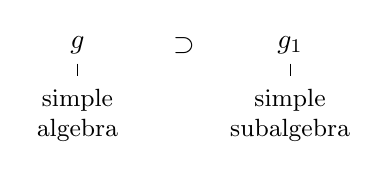
\begin{tikzpicture}[x=1cm,y=1cm]
\node at (0,0) {\(\mathfrak g\)};
\node at (1.35,0) {\(\supset\)};
\node at (2.7,0) {\(\mathfrak g_1\)};
\draw (0,-.23) -- (0,-.39);
\draw (2.7,-.23) -- (2.7,-.39);
\node[align=center,anchor=north,font=\small] at (0,-.43) {simple\\algebra};
\node[align=center,anchor=north,font=\small] at (2.7,-.43) {simple\\subalgebra};
\end{tikzpicture}}\endgroup}\par\smallskip}
\end{GelfandAdjacentEvidence}
\begin{GelfandAdjacentEvidence}{GELFAND-P001227}{3}

\begin{equation*}
\widehat{\mathfrak g}\supset\widehat{\mathfrak g}_1
\end{equation*}

\(M\) --- a representation of \(\widehat{\mathfrak g}\) from category [crossed out] \(O\).
\Unclear{GELFAND-P001227}{category-cancellation}{The mark before \(O\) is crossed out and illegible.}
\end{GelfandAdjacentEvidence}
\begin{GelfandAdjacentEvidence}{GELFAND-P001227}{4}


\(e_i^{\mathfrak g}\), \(e_i^{\mathfrak g_1}\) --- the corresponding \(e_i\),
constr. from \(\mathfrak g\) and \(\mathfrak g_1\).

Consider \(e_i=e_i^{\mathfrak g}-e_i^{\mathfrak g_1}\).

(16) \underline{Theorem.} 1) \(e_i\) [inserted above the line: also] generate a Virasoro alg.

2) \(e_i\) commute with the algebra \(\widehat{\mathfrak g}_i\).
\EvidenceBlock{GELFAND-P001227}{commuting-subscript}{The subscript on \(\widehat{\mathfrak g}\) in item 2 is a dotted \(i\).}{Manuscript notation.}
\end{GelfandAdjacentEvidence}
\begin{GelfandAdjacentEvidence}{GELFAND-P001227}{5}


3) Cent. charge of the alg. \(\{e_i\}\) \(=\)
(cent. charge of \(e_i^{\mathfrak g}\)) \(-\) (cent. charge of \(e_i^{\mathfrak g_1}\)).

[Under “Cent. charge”, linked by two vertical strokes: (cent. element).]
\begin{equation*}
\begin{aligned}
&\int_0^1\prod(t_i-t_j)^\rho
\left(\prod t_i\right)^\alpha\prod(1-t_i)^\beta\,dt_1\ldots dt_m=\\
&\qquad=\prod_{i=1}^{m}\frac{\Gamma(i\rho)}{\Gamma(\rho)}
\prod_{i=0}^{m-1}\frac{\Gamma(1+\alpha+i\rho)\,\Gamma(1+\beta+i\rho)}
{\Gamma(2+\alpha+\beta+(m-1+i)\rho)}.
\end{aligned}\tag{17}
\end{equation*}
\Unclear{GELFAND-P001227}{product-cancellation}{An illegible mark below the second product sign is crossed out.}
\end{GelfandAdjacentEvidence}
\begin{GelfandAdjacentEvidence}{GELFAND-P001227}{6}

\EvidenceBlock{GELFAND-P001227}{integral-conventions}{The exponent on \((t_i-t_j)\) is \(\rho\). The first and third product signs have no written indices. The integral has written bounds \(0\) and \(1\).}{Manuscript notation.}
\end{GelfandAdjacentEvidence}


Special case of a formula of V. Fateev and Dotsenko.


\Needspace{7\baselineskip}
\begin{GelfandAdjacentEvidence}{GELFAND-P001228}{1}
\SourcePage{GELFAND-P001228}{unlabelled}
\(\alpha_+,\alpha_-\), \(\alpha_+\alpha_-=-2\).
\Unclear{GELFAND-P001228}{equality-mark}{The small mark above the equals sign is illegible.}
\end{GelfandAdjacentEvidence}
\begin{GelfandAdjacentEvidence}{GELFAND-P001228}{2}

\begin{equation*}
\begin{aligned}
&\int_0^1
\prod_{\substack{i,j=1\\i<j}}^{n}(t_i-t_j)^{\alpha_+^2}
\prod_{\substack{n+1\le i,j\le n+m\\i<j}}(t_i-t_j)^{\alpha_-^2}
\left(\prod_{i=1}^{n+m}t_i\right)^\beta\\
&\qquad{}\cdot\prod_{\substack{1\le u\le n\\n+1\le v\le m+1}}(t_u-t_v)^{-2}\cdot\\
&\qquad{}\cdot\prod_{1\le i\le n}(z-t_i)^\gamma
\prod_{n+1\le i\le n+m}(z-t_i)^\delta\,dt_1\ldots dt_n.
\end{aligned}\tag{18}
\end{equation*}
\Unclear{GELFAND-P001228}{first-product-cancellation}{Notation is crossed out between \(i,j=1\) and \(i<j\) beneath the first product. Strokes resembling \(i\) and \(j\) are visible. The sign between them is illegible.}
\end{GelfandAdjacentEvidence}
\begin{GelfandAdjacentEvidence}{GELFAND-P001228}{3}

\Unclear{GELFAND-P001228}{mixed-product-cancellation}{An illegible mark is crossed out beneath the two constraints on the mixed product.}
\end{GelfandAdjacentEvidence}
\begin{GelfandAdjacentEvidence}{GELFAND-P001228}{4}

\EvidenceBlock{GELFAND-P001228}{integral-index-mismatch}{The upper bound for \(v\) is written \(m+1\). The final differential is written \(dt_n\).}{Manuscript notation.}
\end{GelfandAdjacentEvidence}
\begin{GelfandAdjacentEvidence}{GELFAND-P001228}{5}


In this form the 2-point correlation fn. of the theory (conformal field theory) is represented.

[crossed out] This gives a [schetnoe?] number of correlation fns.
\Unclear{GELFAND-P001228}{prose-cancellation}{The crossed-out word before “This gives” may read «Если» (Esli).}
\end{GelfandAdjacentEvidence}
\begin{GelfandAdjacentEvidence}{GELFAND-P001228}{6}

\Unclear{GELFAND-P001228}{count-word}{The word before “number” tentatively reads «счетное» (schetnoe). Its ending «етное» is legible and its opening strokes are unclear.}
\end{GelfandAdjacentEvidence}
\begin{GelfandAdjacentEvidence}{GELFAND-P001228}{7}


The real fns. are their analytic continuation to complex \(n\) and \(m\).

\uwave{It is called 4-point} (although it depends only on \(z\)).

[A short stroke leads down from \(z\)] [crossed out] cross-ratio of 4 points on \(CP^1\).
\Unclear{GELFAND-P001228}{marginal-cancellation}{The crossed-out word before “cross-ratio” may read «она» (ona).}
\end{GelfandAdjacentEvidence}
\begin{GelfandAdjacentEvidence}{GELFAND-P001228}{8}

\EvidenceBlock{GELFAND-P001228}{correlation-order}{The upper passage reads “2-point”. The lower passage reads “4-point”, with a raised and underlined х after the numeral.}{Manuscript notation.}
\end{GelfandAdjacentEvidence}



\Needspace{7\baselineskip}
\begin{GelfandAdjacentEvidence}{GELFAND-P001229}{1}
\SourcePage{GELFAND-P001229}{unlabelled}
\underline{\(11/\overline{\underline{\mathrm{XI}}}-85\)  }\qquad
\underline{Gelfand Sem.}

\underline{\underline{Vershik A. M.}}\qquad \underline{Topology of configuration space[?].}
\Unclear{GELFAND-P001229}{title-word}{The legible stem is «пространств» (prostranstv). The inked-over final sign is tentatively «а» (a). A separate dot is visible to its right.}
\end{GelfandAdjacentEvidence}
\begin{GelfandAdjacentEvidence}{GELFAND-P001229}{2}


\(1^{\circ}.\)
\SourceFigure{GELFAND-P001229}{grassmann-membership}{%
\par\smallskip
{\color{black}\begingroup\color{black}\GelfandFitDiagram{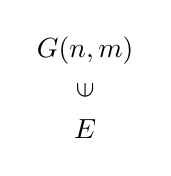
\begin{tikzpicture}
\node at (0,0) {\(G(n,m)\)};
\node[rotate=90] at (0,-.5) {\(\in\)};
\node at (0,-1) {\(E\)};
\end{tikzpicture}}\endgroup}\par\smallskip}
\end{GelfandAdjacentEvidence}
\begin{GelfandAdjacentEvidence}{GELFAND-P001229}{3}

\(e_1,\ldots,e_n\) --- basis in \(\mathbb R^n\)
\begin{equation*}
\tau_E=(Pe_1,\ldots,Pe_n)
\end{equation*}
What is the top. stratum in \(G(n,m)\), where \(\tau_E\) has a given combinat. type?

\(2^{\circ}.\) Combinat. theory of convex polyhedra in \(\mathbb R^n\).

2 polyhedra \(V_1,V_2\) with ordered (numbered) vertices (\(n\) of them)
[crossed out] have the same combinat. type if their faces correspond to each other.
\Incomplete{GELFAND-P001229}{cancelled-type}{The crossed-out passage after “\(n\) of them” is undeciphered.}
\end{GelfandAdjacentEvidence}
\begin{GelfandAdjacentEvidence}{GELFAND-P001229}{4}


Grassmannization of the problem.

In \(\mathbb R^n\) consider a subspace (\(m\)-dimensional) \(E\)
\begin{equation*}
S=\omega(e_1,\ldots,e_n)\quad\text{--- simplex}
\end{equation*}
\EvidenceBlock{GELFAND-P001229}{simplex-symbol}{The sign after the equals sign is \(\omega\).}{Manuscript notation.}
\end{GelfandAdjacentEvidence}
\begin{GelfandAdjacentEvidence}{GELFAND-P001229}{5}

The projection of \(S\) onto \(E\) --- polyhedron (convex)

\underline{Ex.:} obtain combinatorially any polyhedron of dim. \(m\) with \(n\) vertices

On \(G(n,m)\) consider the partition into subsets where the polyhedra carried by the subspace are combinatorially equivalent.
\EvidenceBlock{GELFAND-P001229}{subspace-abbreviation}{The abbreviation after “carried” is «подпр-вом» (podpr-vom, “by the subspace”).}{Manuscript notation.}
\end{GelfandAdjacentEvidence}
\begin{GelfandAdjacentEvidence}{GELFAND-P001229}{6}


What is the topology of these pieces?

\(3^{\circ}.\)
\SourceFigure{GELFAND-P001229}{matrix-hatching}{%
\par\smallskip
{\color{black}\(\begin{array}{c}
\left(\begin{array}{@{}ccc@{}}
x_{11}&\cdots&x_{1n}\\
x_{21}&\cdots&x_{2n}\\
x_{31}&\cdots&x_{3n}\\
\hline
\multicolumn{3}{c}{\text{\tikz[x=.65cm,y=.40cm]{
\draw (0,.02)--(.37,.26)--(.24,.04)--(.74,.24)--(.61,.02)--(1.13,.24)--(1.00,.03)--(1.54,.22)--(1.39,.01)--(1.89,.23);}}}
\end{array}\right)
\qquad
\begin{pmatrix}
x'_{11}&\cdots&x'_{1n}\\
x'_{21}&\cdots&x'_{2n}\\
x'_{31}&\cdots&x'_{3n}
\end{pmatrix}\\[3pt]
\text{--- 2 matrices }3\times n
\end{array}\)}\par\smallskip
A rule and looping hatching lie under the third row of the first matrix. The purpose of the hatching is unclear. The second matrix has neither mark.}
\end{GelfandAdjacentEvidence}


Let all minors be \(\ne0\) and have the same signs for \(x\) and \(x'\).

Does there exist a homotopy \(x(t)\) of matrices with \(x(0)=x\), \(x(1)=x'\)


\Needspace{7\baselineskip}
\begin{GelfandAdjacentEvidence}{GELFAND-P001230}{1}
\SourcePage{GELFAND-P001230}{15}
in the same class?
\begin{gather*}
n\le7\ \Rightarrow\ \text{possible}\\
n=19\ \Rightarrow\ \text{impossible!}\qquad\text{(N. E. Mnëv)}
\end{gather*}
Configurations also make sense in \(\mathbb RP^n\) and one needs to supplement.
\EvidenceBlock{GELFAND-P001230}{configuration-end}{The final word reads «дополнять» (dopolnyat', “to supplement”).}{Manuscript notation.}
\end{GelfandAdjacentEvidence}
\begin{GelfandAdjacentEvidence}{GELFAND-P001230}{2}


One needs to [probe?] the consequences (by projection) and there is a bound on how many one needs to take to have enough.
\Unclear{GELFAND-P001230}{consequences-verb}{The joined strokes tentatively read «пощупать» (poshchupat', “to probe”). The following word “consequences” is legible.}
\end{GelfandAdjacentEvidence}
\begin{GelfandAdjacentEvidence}{GELFAND-P001230}{3}

\EvidenceBlock{GELFAND-P001230}{consequences-parenthesis}{The parenthesis reads «проектированием» (proektirovaniem, “by projection”). It is followed by “and there is a bound.”}{Manuscript notation.}
\end{GelfandAdjacentEvidence}
\begin{GelfandAdjacentEvidence}{GELFAND-P001230}{4}


The topology can be that of any algebraic var.!

(This is over \(\mathbb R\))

over \(C\) the analogue is computing \(\pi_1\).

It is interesting what the convex analogue is over \(C\).

\underline{Steinitz's thm.}: characterization of the 1-dim. skeleton of a convex polyhedron

(see any textbook of convex geom.) (in \(\mathbb R^3\))

\underline{Corollary}: the space of polyhedra of a given combinat. type in \(\mathbb R^3\) is contractible.

\underline{But}: in \(\mathbb R^4\) there already exist even simplicial polyhedra
with more or less any [crossed out] topology of combinat. type.
\Incomplete{GELFAND-P001230}{topology-cancel}{The crossed-out word between “any” and “topology” is undeciphered.}
\end{GelfandAdjacentEvidence}
\begin{GelfandAdjacentEvidence}{GELFAND-P001230}{5}


\uwave{Problem}: we want to construct a field of polyhedra on a manifold! (in each tangent sp.).
There was [crossed out] a classific. problem for this one.
\Incomplete{GELFAND-P001230}{classification-cancel}{The crossed-out passage after “There was” is undeciphered.}
\end{GelfandAdjacentEvidence}
\begin{GelfandAdjacentEvidence}{GELFAND-P001230}{6}


\uwave{Matroids} [m.?] Given a lattice. It is called a \uwave{geometric lattice},
if it is
\begin{enumerate}
\item[1)] Semimodular
\item[2)] Finite (\(\forall\) elem. \(=\sup\) of finitely many atoms)
\end{enumerate}
[Below this line:] atoms --- those immed. after zero.
\Unclear{GELFAND-P001230}{matroid-mark}{The retraced mark after “Matroids” tentatively reads «м.» (m.). Its function is unclear.}
\end{GelfandAdjacentEvidence}
\begin{GelfandAdjacentEvidence}{GELFAND-P001230}{7}


Config. --- geom. lattice.

Conversely, let a geom. lattice be given. When is it given by a config.?

\SourceFigure{GELFAND-P001230}{fano-diagram}{%
\par\smallskip
{\color{black}\begingroup\color{black}\GelfandFitDiagram{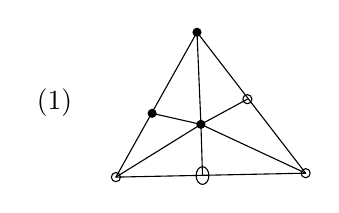
\begin{tikzpicture}[x=1cm,y=1cm,line cap=round,line join=round]
\coordinate (T) at (1.03,1.84);
\coordinate (L) at (0,0);
\coordinate (R) at (2.41,.05);
\coordinate (TL) at (.46,.81);
\coordinate (TR) at (1.67,.99);
\coordinate (B) at (1.1,.02);
\coordinate (C) at (1.08,.67);
\node[anchor=east] at (-.43,.95) {(1)};
\draw (L)--(T)--(R)--cycle;
\draw (T)--(C)--(B) (L)--(C)--(TR) (R)--(C)--(TL);
\foreach \point in {T,TL,C} \fill (\point) circle[radius=1.65pt];
\foreach \point in {L,R,TR} \draw (\point) circle[radius=1.65pt]; \draw (B) ellipse[x radius=2.3pt,y radius=3.2pt];
\end{tikzpicture}}\endgroup}\par\smallskip
Seven marked points and three interior lines are visible. The lower middle loop extends below the base. No separate line through the three points on the sides is visible.}
\end{GelfandAdjacentEvidence}
\begin{GelfandAdjacentEvidence}{GELFAND-P001230}{8}

(Fano config.)\qquad over \(\mathbb R,\mathbb Z\) is not realizable.

A faithful rep. of a lattice \(=\) a map from it
\begin{equation*}
a:\Gamma\longrightarrow\mathcal L(F^n)\quad\text{--- lattice of subspaces,}
\end{equation*}
such that
\begin{equation*}
\gamma_1<\gamma_2\ \Rightarrow\ a(\gamma_1)<a(\gamma_2)
\end{equation*}
and \(\sup\) is preserved

(1) is not realizable [crossed out] over \(\mathbb R\), but over \(\mathbb Z_2\) realiz..
\Unclear{GELFAND-P001230}{realization-cancel}{The crossed-out mark before “over” is illegible.}
\end{GelfandAdjacentEvidence}



\Needspace{7\baselineskip}
\begin{GelfandAdjacentEvidence}{GELFAND-P001231}{1}
\SourcePage{GELFAND-P001231}{unlabelled}
A faithful rep. exists for config. (1):
\begin{equation*}
?\qquad m=4,\quad E,\quad \underline F,\quad \underline{\mathbb R^6}
\end{equation*}
\EvidenceBlock{GELFAND-P001231}{opening-symbols}{The line with the question mark lists \(m=4\), \(E\), \(F\) and \(\mathbb R^6\) separately.}{Manuscript notation.}
\end{GelfandAdjacentEvidence}
\begin{GelfandAdjacentEvidence}{GELFAND-P001231}{2}


Realizability problem \(\Leftrightarrow\) problem of solving a system of algebraic inequalities.
\EvidenceBlock{GELFAND-P001231}{inequalities-reading}{The abbreviation after “algebraic” is «нер-в.» (ner-v., “inequalities”).}{Manuscript notation.}
\end{GelfandAdjacentEvidence}
\begin{GelfandAdjacentEvidence}{GELFAND-P001231}{3}


\uwave{Nontriv. work on lattices:} (according to Gelfand)
\EvidenceBlock{GELFAND-P001231}{lattice-heading}{The first abbreviation in the heading is «Нетрив.» (Netriv., “Nontriv.”).}{Manuscript notation.}
\end{GelfandAdjacentEvidence}
\begin{GelfandAdjacentEvidence}{GELFAND-P001231}{4}


Dedekind: invented it

Kurosh, Ore.

von Neumann;

Gelfand, Ponomarev:

[In the left margin: \uwave{Vershik's add.:}]
\uwave{Pudlák and Tůma} (Czechs): every finite lattice embeds into the partition lattice of a finite set (very difficult theorem).

(\(\inf\) and \(\sup\) --- [crossed out] intersection and union)
\Incomplete{GELFAND-P001231}{inf-sup-cancel}{The word after “inf and sup” is crossed out and undeciphered.}
\end{GelfandAdjacentEvidence}
\begin{GelfandAdjacentEvidence}{GELFAND-P001231}{5}


\(0\) --- partition into points.

\medskip
\underline{\underline{Feigin B.}}\qquad\underline{On strings} [crossed out] (continued).
\Unclear{GELFAND-P001231}{string-heading-cancel}{The crossed-out vertical mark after “On strings” is undeciphered.}
\end{GelfandAdjacentEvidence}
\begin{GelfandAdjacentEvidence}{GELFAND-P001231}{6}


\underline{Operator theory of strings.}

\underline{Dual amplitudes.} Consider a collision of particles

\SourceFigure{GELFAND-P001231}{scattering-diagram}{%
\par\smallskip
{\color{black}\begingroup\color{black}\GelfandFitDiagram{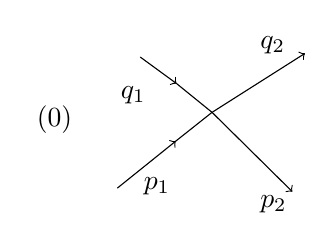
\begin{tikzpicture}[x=1cm,y=.96cm,line cap=round]
\node at (-2,0) {(0)};
\coordinate (lowerin) at (-1.2,-.90);
\coordinate (upperin) at (-.91,.83);
\coordinate (crossing) at (0,.10);
\coordinate (upperout) at (1.18,.88);
\coordinate (lowerout) at (1.02,-.95);
\draw[->] (lowerin)--(-.46,-.28);
\draw[->] (-.46,-.28)--(crossing)--(upperout);
\draw[->] (upperin)--(-.45,.48);
\draw[->] (-.45,.48)--(crossing)--(lowerout);
\node[below] at (-.70,-.63) {\(p_1\)};
\node[left] at (-.72,.33) {\(q_1\)};
\node[above] at (.77,.74) {\(q_2\)};
\node[below] at (.78,-.87) {\(p_2\)};
\end{tikzpicture}}\endgroup}\par\smallskip}
\end{GelfandAdjacentEvidence}
\begin{GelfandAdjacentEvidence}{GELFAND-P001231}{7}


Let the masses all be the same and the total momentum \(=0\)

All are vectors in space/time
\begin{equation*}
\begin{cases}
p_1+q_1=p_2+q_2,\\
p_1^2=q_1^2=p_2^2=q_2^2=m^2
\end{cases}
\qquad p_j,q_j\in\mathbb R^4.
\tag{1}
\end{equation*}
\EvidenceBlock{GELFAND-P001231}{mass-shell-overwrite}{The final form of the overwritten letter and its subscript in the penultimate square reads \(q_2\).}{Manuscript notation.}
\end{GelfandAdjacentEvidence}
\begin{GelfandAdjacentEvidence}{GELFAND-P001231}{8}


Let an \(S\)-matrix characterizing this collision be given,
\begin{equation*}
S(p_1,q_1,p_2,q_2)\tag{2}
\end{equation*}
Mandelstam variables:
\begin{equation*}
\begin{cases}
s=(p_1+q_1)^2,\\
t=(p_1-p_2)^2\\
u\ \text{[crossed out]}=(p_1-q_2)^2
\end{cases}\tag{3}
\end{equation*}
\Unclear{GELFAND-P001231}{mandelstam-u-cancel}{An illegible mark between \(u\) and the equals sign is crossed out.}
\end{GelfandAdjacentEvidence}
\begin{GelfandAdjacentEvidence}{GELFAND-P001231}{9}

[To the right of (3):] (Relativistically invariant pairwise scalar products are given)

dependent:
\begin{equation*}
s+t+u=4m^2\tag{4}
\end{equation*}
Define \(A(s,t)\) (\(=\) expression for \(S\) in terms of \(s,t\))

\uwave{Requirement}:
\begin{equation*}
1)\quad A\text{ is analytic in }s,t\quad\text{[crossed out]}\tag{5}
\end{equation*}
\Unclear{GELFAND-P001231}{analytic-tail}{A mark after \(t\) is crossed out. Its reading is unresolved.}
\end{GelfandAdjacentEvidence}



\Needspace{7\baselineskip}
\begin{GelfandAdjacentEvidence}{GELFAND-P001232}{1}
\SourcePage{GELFAND-P001232}{16}
2) \(A\) is symmetric in \(s,t\) (indep. of the order)

3) For fixed \(t\) the fn. \(A(s,t)\) has in \(s\) only simple poles,
and [inserted between words: 4)] the locations of the poles do not depend on \(t\). Usually one writes:
\begin{equation*}
A(s,t)=\sum_{n=0}^{\infty}\frac{R_n(t)}{n-\alpha(s)}\tag{6}
\end{equation*}
5) \(R_n(t)\) --- polynomial

The graph of \(\alpha(s)\) is called a Regge trajectory.

It turns out that from 1)---5) we uniquely determine the form of the fn. \(A\):
\begin{equation*}
A(s,t)=\frac{\Gamma(-\alpha(s))\Gamma(-\alpha(t))}{\Gamma(-\alpha(s)-\alpha(t))}
=B(-\alpha(s),-\alpha(t))\tag{7}
\end{equation*}
It follows from analysis of the exper. data that
\begin{equation*}
\alpha(s)\quad\text{--- linear fn.}\tag{8}
\end{equation*}
\(A\) is called the Veneziano amplitude, or dual amplitude, and conds. 1)---5) are called \underline{duality conditions}.

Operator method: we want to write \(A(s,t)\) as an operator expectation
\begin{equation*}
\langle0|V(t)V(s)|0\rangle,\tag{9}
\end{equation*}
where \(\langle0|\) --- vac. vector in some space, \(V(t)\) --- operators.

Another form of (7):
\begin{equation*}
S(p_1,p_2,p_3,p_4)=\int_0^1
x^{-2\langle p_1,p_2\rangle}(1-x)^{-2\langle p_2,p_3\rangle}
(x(1-x))^{-1-m^2}\,dx\tag{10}
\end{equation*}
Here

\SourceFigure{GELFAND-P001232}{amplitude-arrow-convention}{%
\par\smallskip
{\color{black}\begingroup\color{black}\GelfandFitDiagram{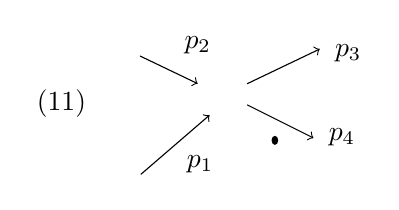
\begin{tikzpicture}[x=1cm,y=1cm,line cap=round]
\node at (-2.1,0) {(11)};
\draw[->] (-1.1,.60)--(-.37,.25);
\draw[->] (-1.09,-.90)--(-.22,-.15);
\draw[->] (.26,.25)--(1.18,.69);
\draw[->] (.26,-.02)--(1.1,-.44);
\node[above] at (-.37,.50) {\(p_2\)};
\node[below] at (-.34,-.54) {\(p_1\)};
\node[right] at (1.25,.64) {\(p_3\)};
\node[right] at (1.17,-.43) {\(p_4\)};
\fill (.61,-.47) ellipse[x radius=1.2pt,y radius=1.65pt];
\end{tikzpicture}}\endgroup}\par\smallskip
An ink mark is visible beside the lower-right arrow. Its relation to the arrow is unclear.}
\end{GelfandAdjacentEvidence}
\begin{GelfandAdjacentEvidence}{GELFAND-P001232}{2}

\begin{equation*}
p_1+p_2+p_3+p_4=0.
\end{equation*}
Similarly one can write amplitudes for a greater number of particles,
for example:
\begin{equation*}
A(p_1,p_2,p_3,p_4,p_5)\cong\int\int_0^1
x^{\cdots}y^{\cdots}(1-x)^{\cdots}(1-y)^{\cdots}(1-xy)^{\cdots}\,dx\,dy\tag{12}
\end{equation*}
This amplitude has not been calculated in general, only for some special values of the \underline{scalar products}.

The space is generated by a finite set of oscillators connected as in a string. A finite number will not do!.
\EvidenceBlock{GELFAND-P001232}{finite-oscillators}{The first sentence says “finite”. The second says “A finite number will not do!”}{Manuscript notation.}
\end{GelfandAdjacentEvidence}
\begin{GelfandAdjacentEvidence}{GELFAND-P001232}{3}


Consider the algebra with generators
\begin{equation*}
a_m^\mu,x^\mu,\quad \mu=0,1,\ldots,d,\quad
\text{[crossed out]}\tag{13}
\end{equation*}
\Incomplete{GELFAND-P001232}{generators-cancel}{The notation after \(d\) in (13) is crossed out and undeciphered.}
\end{GelfandAdjacentEvidence}

where \(d\) --- dim. of the space


\Needspace{7\baselineskip}
\begin{GelfandAdjacentEvidence}{GELFAND-P001233}{1}
\SourcePage{GELFAND-P001233}{unlabelled}
\begin{equation*}
\relax [a_m^\mu,a_n^\nu]=m g^{\mu\nu}\delta_{m,-n}\tag{14}
\end{equation*}
\(m,n\) --- integers
\begin{equation*}
a_0^\mu=p^\mu\tag{15}
\end{equation*}
\begin{equation*}
\relax [x^\mu,p^\nu]=i g^{\mu\nu}\tag{16}
\end{equation*}
\EvidenceBlock{GELFAND-P001233}{momentum-superscript}{The final form of the overwritten superscript on \(p\) in (16) reads \(\nu\).}{Manuscript notation.}
\end{GelfandAdjacentEvidence}
\begin{GelfandAdjacentEvidence}{GELFAND-P001233}{2}

\begin{equation*}
\relax [x^\mu,a_m^\nu]=0,\quad m\ne0\tag{17}
\end{equation*}
Meaning of the generators \(x^\mu,a_m^\mu\):

[Crossed out: \(p^\mu\) --- undeciphered]
\Unclear{GELFAND-P001233}{coordinates-cancel}{The crossed-out notation begins with \(p^\mu\). The remaining signs are illegible.}
\end{GelfandAdjacentEvidence}
\begin{GelfandAdjacentEvidence}{GELFAND-P001233}{3}

\((x^\mu,p^\mu)\) --- coord. and momentum of the center of gravity of the flying string, \(a_m^\mu\) --- Fourier series expansion of everything else.

Put:
\begin{equation*}
P^\mu(\theta)=\sum_{-\infty}^{+\infty}a_m^\mu e^{-im\theta},\tag{18}
\end{equation*}
(momentum of the point with param. \(\theta\))
\begin{equation*}
Q^\mu(\theta)=x^\mu+a_0^\mu\theta+
 i\sum_{\substack{n=-\infty\\n\ne0}}^{\infty}\frac1n a_{[m?]}^\mu e^{-in\theta}.\tag{19}
\end{equation*}
\Unclear{GELFAND-P001233}{fourier-index}{The overwritten subscript on \(a\) tentatively reads \(m\), with \(n\) also possible. The summation index and the index in the exponent are \(n\).}
\end{GelfandAdjacentEvidence}
\begin{GelfandAdjacentEvidence}{GELFAND-P001233}{4}

Then the commutation relations hold:
\begin{equation*}
\relax [Q_\mu(\theta),P_\nu(\theta')]=2\pi i g_{\mu\nu}\delta(\theta-\theta')\tag{20}
\end{equation*}
\begin{equation*}
\relax [P_\mu(\theta),P_\nu(\theta')]=2\pi i g_{\mu\nu}\delta'(\theta-\theta')\tag{21}
\end{equation*}
\begin{equation*}
\relax [Q_\mu(\theta),Q_\nu(\theta')]=-\pi i g_{\mu\nu}\varepsilon(\theta-\theta'),\tag{22}
\end{equation*}
where \(\varepsilon\) --- Heaviside fn.
\Unclear{GELFAND-P001233}{heaviside-convention}{The line reads “where \(\varepsilon\) is the Heaviside fn.” Its normalization is unspecified here.}
\end{GelfandAdjacentEvidence}
\begin{GelfandAdjacentEvidence}{GELFAND-P001233}{5}

\begin{equation*}
L_m\overset{\mathrm{def}}{=}\frac1{4\pi}\int_0^{2\pi}
e^{im\theta}:P^2(\theta):\,d\theta\tag{23}
\end{equation*}
Then one obtains a representation of the Virasoro algebra
\begin{equation*}
\relax [L_m,L_n]=(m-n)L_{m+n}+\frac d{12}(m^3-m)\delta_{m,-n}\tag{24}
\end{equation*}
\Unclear{GELFAND-P001233}{central-dimension}{The central coefficient is written \(\frac{d}{12}\).}
\end{GelfandAdjacentEvidence}


\uwave{Exercise}: verify this.

Incidentally,
\begin{equation*}
L_0=\frac12a_0^2+\sum_{n=1}^{\infty}a_{-n}a_n\tag{25}
\end{equation*}


\Needspace{7\baselineskip}
\begin{GelfandAdjacentEvidence}{GELFAND-P001234}{1}
\SourcePage{GELFAND-P001234}{17}
\begin{equation*}
2L_m={:}\sum_{r+s=m}a_ra_s{:}\tag{26}
\end{equation*}
\uwave{Vertex operator}: put
\begin{equation*}
V(k,\theta)=\exp\langle ik,Q(\theta)\rangle,\tag{27}
\end{equation*}
where \(k\) --- a vector, then
\begin{equation*}
V(k)=V(k,0)=
\exp\left\langle k,\sum_{n=1}^{\infty}\frac{a_{-n}}n\right\rangle
\exp(ikx)
\exp\left\langle-k,\sum_{n=1}^{\infty}\frac{a_n}n\right\rangle
\tag{28}
\end{equation*}
\EvidenceBlock{GELFAND-P001234}{vertex-insertion}{The factor \(\exp(ikx)\) is inserted above the line. The insertion strokes converge between the two exponentials.}{Manuscript notation.}
\end{GelfandAdjacentEvidence}
\begin{GelfandAdjacentEvidence}{GELFAND-P001234}{2}

and
\begin{equation*}
V(k,\theta)=\exp(i\theta L_0)V(k)\exp(-i\theta L_0).\tag{29}
\end{equation*}
Next,

[Crossed out before (30)]
\begin{equation*}
\relax [L_n-L_0,V(k)]=\frac{nk^2}2V(k).\tag{30}
\end{equation*}
\Incomplete{GELFAND-P001234}{commutator-cancel}{The notation before the commutator in (30) is crossed out and undeciphered.}
\end{GelfandAdjacentEvidence}
\begin{GelfandAdjacentEvidence}{GELFAND-P001234}{3}


Consider a series of interactions:

\SourceFigure{GELFAND-P001234}{interaction-chain}{%
\par\smallskip
{\color{black}\begingroup\color{black}\GelfandFitDiagram{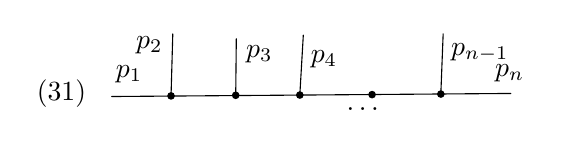
\begin{tikzpicture}[x=.74cm,y=.78cm,line cap=round]
\node at (-.86,.05) {(31)};
\draw (0,0)--(6.85,.05);
\draw (1.02,.01)--(1.05,1.02) (2.13,.02)--(2.14,.94)
      (3.23,.024)--(3.29,1.0) (5.65,.04)--(5.69,1.02);
\foreach \x/\y in {1.02/.01,2.13/.02,3.23/.024,4.47/.031,5.65/.04}
   \fill (\x,\y) circle[radius=1.38pt];
\node[above] at (.30,.06) {\(p_1\)};
\node[left] at (1.04,.83) {\(p_2\)};
\node[right] at (2.14,.69) {\(p_3\)};
\node[right] at (3.25,.61) {\(p_4\)};
\node[right] at (5.66,.72) {\(p_{n-1}\)};
\node[above] at (6.83,.08) {\(p_n\)};
\node[below] at (4.31,-.02) {\(\ldots\)};
\end{tikzpicture}}\endgroup}\par\smallskip}
\end{GelfandAdjacentEvidence}
\begin{GelfandAdjacentEvidence}{GELFAND-P001234}{4}


and from such a picture construct the amplitude:
\begin{equation*}
\langle0|V(p_2)D(s_2)V(p_3)D(s_3)\ldots D(s_{n-2})V(p_{n-1})|0\rangle,
\tag{32}
\end{equation*}
\EvidenceBlock{GELFAND-P001234}{last-propagator-index}{The overwritten numeral in the last argument of \(D\) reads \(2\). The argument is written \(s_{n-2}\).}{Manuscript notation.}
\end{GelfandAdjacentEvidence}

where \(p\) --- the same as \(k\),
\begin{equation*}
\begin{aligned}
s_2&=(p_2+p_1)^2\\
s_3&=(p_3+p_2+p_1)^2,\\
&\ldots
\end{aligned}\tag{33}
\end{equation*}
\begin{equation*}
D(s)=\int_0^1 x^{L_0-\alpha(s)-1}(1-x)^{\alpha(0)-1}\,dx,\tag{34}
\end{equation*}
where \(\alpha(s)\) --- linear fn. (Regge trajectory).

(32) --- dual amplitude. It should agree with \(A\), when there are 4 vertices.

Expand \(V(k,\theta)\) in a Fourier series:
\begin{equation*}
V(k,\theta)=\sum V_n(k)e^{-in\theta}.\tag{35}
\end{equation*}
There are operators \(a_i^\mu\) and \(a_0^\mu\) and vacuum vectors
\(|0,p\rangle\), satisfying the condition


\Needspace{7\baselineskip}
\begin{GelfandAdjacentEvidence}{GELFAND-P001235}{1}
\SourcePage{GELFAND-P001235}{unlabelled}
\begin{equation*}
a_i^\mu|0,p\rangle=0,\quad\text{if }i>0,
\tag*{$(36)_i$}
\end{equation*}
\begin{equation*}
a_0^\mu|0,p\rangle=
\text{[crossed out]}\ p^\mu\,\text{[crossed out]}\ |0,p\rangle.
\tag*{$(36)_0$}
\end{equation*}
\Unclear{GELFAND-P001235}{vacuum-cancel-left}{crossed-out writing before $p^\mu$}
\end{GelfandAdjacentEvidence}
\begin{GelfandAdjacentEvidence}{GELFAND-P001235}{2}

\Unclear{GELFAND-P001235}{vacuum-cancel-right}{crossed-out sign after $p^\mu$}
\end{GelfandAdjacentEvidence}
\begin{GelfandAdjacentEvidence}{GELFAND-P001235}{3}

(the vacua are indexed by momentum vectors)

We obtain the space
\begin{equation*}
\bigoplus_p H(p)
\tag{37}
\end{equation*}
The vertex operator acts as follows:
\begin{equation*}
V_n(k):H(p)\longrightarrow H(p+k).
\tag{38}
\end{equation*}
Commutation relations:

[Crossed out: illegible]
\Incomplete{GELFAND-P001235}{commutator-cancel}{The crossed-out writing under “Commutation relations” is illegible.}
\end{GelfandAdjacentEvidence}
\begin{GelfandAdjacentEvidence}{GELFAND-P001235}{4}

\begin{equation*}
\relax [a_m^\mu,V_n(k)]=V_{n+m}(k)\cdot k_\mu
\tag{39}
\end{equation*}
\EvidenceBlock{GELFAND-P001235}{commutator-index}{In the factor \(k_\mu\) in (39), \(\mu\) is written below the baseline.}{Manuscript notation.}
\end{GelfandAdjacentEvidence}
\begin{GelfandAdjacentEvidence}{GELFAND-P001235}{5}


[Crossed out: $V_n(k_1)|0,p\rangle$ / $V_1(k_1)|0,p\rangle$\textsuperscript{?}] Set
\Unclear{GELFAND-P001235}{vertex-cancel}{The crossed-out expression shows \(V\), \((k_1)\) and \(\lvert 0,p\rangle\). The subscript on \(V\) may be \(n\) or \(1\).}
\end{GelfandAdjacentEvidence}
\begin{GelfandAdjacentEvidence}{GELFAND-P001235}{6}

\begin{equation*}
\langle0,p+k_1+k|V_{-n}(k_2)V_n(k_1)|0,p\rangle=A_n\qquad\text{(these are numbers)}
\tag{40}
\end{equation*}
\EvidenceBlock{GELFAND-P001235}{bra-last-momentum}{The bra in (40) has \(p+k_1+k\). The final \(k\) has no written subscript.}{Manuscript notation.}
\end{GelfandAdjacentEvidence}


Then
\begin{equation*}
\sum A_n z^n=(1-z)^{\langle k_1,k_2\rangle}.
\tag{41}
\end{equation*}
This follows by a direct computation. The reader is asked to verify (41) as an exercise.


\Needspace{7\baselineskip}
\begin{GelfandAdjacentEvidence}{GELFAND-P001236}{1}
\SourcePage{GELFAND-P001236}{26}
\underline{18 Nov. 1985}\qquad \underline{Gelfand Seminar}

\underline{B. Feigin} (continued).

The $L_i$ generate the Virasoro algebra. Let there be a large space on which this algebra acts.

Eigenvectors of $L_0$ are weight vectors.

By the commutation relations, $L_i$ acts on the space of weight vectors.

(see (24) on p.~17, left)

Highest [crossed out: vector?\textsuperscript{?}] weight: a vector that cannot be raised any further
\Unclear{GELFAND-P001236}{highest-cancel}{The crossed-out word may read «вектор» (vektor, “vector”). The strokes obscure the middle of the word.}
\end{GelfandAdjacentEvidence}
\begin{GelfandAdjacentEvidence}{GELFAND-P001236}{2}

\begin{equation*}
\widetilde{\mathcal H}=\{v\mid L_0v=v,\quad L_iv=0\ \text{for }i>0\}.\qquad\text{(weight 1)}
\tag{1}
\end{equation*}
\begin{equation*}
\overline{\mathcal H}=\{v\in\widetilde{\mathcal H},\quad v=L_i v',\ i<0\},
\tag{2}
\end{equation*}
[At right:] Here $v'$ is an arbitrary weight vector from the large space.

(the space of “spurions,” a term used by physicists some 15 years ago)
\begin{equation*}
\mathcal H\overset{\mathrm{def}}{=}\widetilde{\mathcal H}/\overline{\mathcal H}
\tag{3}
\end{equation*}
\begin{equation*}
\prod_{i=1}^N a_{m_i}^{\mu_i}|0,p\rangle
\tag{4}
\end{equation*}
[At right:] (space of states)

a large module over the Virasoro algebra
\begin{equation*}
L_{-1}v'=v\quad\Rightarrow\quad v'\text{ has weight }2:\quad L_0v'=2v'
\tag{5}
\end{equation*}
\EvidenceBlock{GELFAND-P001236}{weight-two}{In (5) the manuscript has \(L_{-1}v'=v\), “\(v'\) has weight 2” and \(L_0v'=2v'\).}{Manuscript notation.}
\end{GelfandAdjacentEvidence}
\begin{GelfandAdjacentEvidence}{GELFAND-P001236}{3}


The aim is to quotient by the diffeomorphism group throughout the space, but a central extension acts, and the centre acts nontrivially.

Another procedure is proposed for obtaining “invariant” vectors. They are invariant under one half, then we quotient by the action of the others and discard them.

The Virasoro algebra disappears, leaving the space of invariants.

We want to

I. Construct a space generated by $d-2$ oscillators.

II. Prove that all vectors in $\widetilde{\mathcal H}/\overline{\mathcal H}$ have norm $>0$.

(this does not hold in the original $d$-dimensional space)

(absence of \underline{tachyons\textsuperscript{?}})
\EvidenceBlock{GELFAND-P001236}{tachyon-word}{The underlined word reads «тахионов» (takhionov, “tachyons”).}{Manuscript notation.}
\end{GelfandAdjacentEvidence}


All of this is achieved in dimension 26.


\Needspace{7\baselineskip}
\begin{GelfandAdjacentEvidence}{GELFAND-P001237}{1}
\SourcePage{GELFAND-P001237}{unlabelled}
Vertex operators
\begin{equation*}
X(p,z)=\exp\left(p_\mu\cdot\sum_{n=1}^{\infty}a_{-n}^\mu z^n\right)D_p
\exp\left(-p_\mu\sum_{n=1}^{\infty}\frac{a_n^\mu}{n}z^{-n}\right),
\tag{6}
\end{equation*}
\EvidenceBlock{GELFAND-P001237}{left-exponential-normalization}{The left exponential in (6) has \(a_{-n}^{\mu}z^n\), with no fraction bar or denominator.}{Manuscript notation.}
\end{GelfandAdjacentEvidence}
\begin{GelfandAdjacentEvidence}{GELFAND-P001237}{2}


where the operators $D_p$ are defined by the formulas
\begin{equation*}
D_p|0,k\rangle=|0,k+p\rangle,\quad [D_p,a_n^\mu]=0,\ n\ne0.
\tag{7}
\end{equation*}
Correlation function
\begin{equation*}
\begin{aligned}
&\langle0,k+\textstyle\sum p_i|X(z_1,p_1)\ldots X(z_n,p_n)|0,k\rangle\\
&\qquad=\prod_{j>1}\left(1-\frac{z_j}{z_i}\right)^{\langle p_i,p_j\rangle}.
\end{aligned}
\tag{8}
\end{equation*}
\EvidenceBlock{GELFAND-P001237}{product-index}{The index under the product is \(j>1\). The final sign has the baseline foot of the numeral \(1\).}{Manuscript notation.}
\end{GelfandAdjacentEvidence}
\begin{GelfandAdjacentEvidence}{GELFAND-P001237}{3}


Expanding $X(z,p)$ in a series gives
\begin{equation*}
X(z,p)=\sum X_i(p)z^i
\tag{9}
\end{equation*}
(this defines the operators $X_i(p)$)

We want to construct 24 oscillators.

Next we will construct the operators
\begin{equation*}
\int X(p,z)\frac{dz}{z},
\tag{10}
\end{equation*}
which commute with the Virasoro algebra when $\langle p,p\rangle=2$.
\begin{equation*}
\begin{aligned}
&\text{In }\mathbb R^{26}\text{ we want to have }p_1,\ldots,p_n:\quad\langle p_i,p_i\rangle=2\\
&\langle p_i,p_j\rangle=A_{ij}\in\mathbb Z,\quad A_{ij}<0.
\end{aligned}
\tag{11}
\end{equation*}
[In the left margin: crossed-out vertical sign\textsuperscript{?}]
\Unclear{GELFAND-P001237}{cartan-margin-cancel}{crossed-out vertical sign}
\end{GelfandAdjacentEvidence}
\begin{GelfandAdjacentEvidence}{GELFAND-P001237}{4}


\EvidenceBlock{GELFAND-P001237}{cartan-diagonal}{The manuscript has \(A_{ij}<0\). There is no index restriction written beside the inequality.}{Manuscript notation.}
\end{GelfandAdjacentEvidence}


Then the operators
\begin{equation*}
e_i=\int X(p_i,z)\frac{dz}{z},\quad f_i=\int X(-p_i,z)\frac{dz}{z}
\tag{12}
\end{equation*}
generate an action of the Kac–Moody algebra with Cartan matrix $A_{ij}$ on the space. We must also set
\begin{equation*}
h_i|0,k\rangle=\langle k,p_i\rangle|0,k\rangle
\tag{13}
\end{equation*}
\underline{Read} the \underline{article by Macdonald} (the beginning), \underline{Sem. Bourbaki}.

Use it to study Lie algebras.

[In the left margin: I.M.G.] The largest finite simple group has $\sim10^{54}$ elements. It is related to strings!

[Added at right:] (Monster “Moonshine”)

Moonshine

(there is work by Frenkel, Lepowsky and someone else)

Somehow one obtains a fundamental representation of the Kac–Moody algebra.


\Needspace{7\baselineskip}
\begin{GelfandAdjacentEvidence}{GELFAND-P001238}{1}
\SourcePage{GELFAND-P001238}{27}
In $\mathbb R^{26}$ consider the metric $\langle-1,1,1,\ldots,1\rangle$,

[Crossed out: nulev…?] vector of length 0, [crossed out: illegible]
\Unclear{GELFAND-P001238}{null-cancel-before}{The crossed-out fragment tentatively reads «нулев…» (nulev…). The ending is illegible.}
\end{GelfandAdjacentEvidence}
\begin{GelfandAdjacentEvidence}{GELFAND-P001238}{2}

\Incomplete{GELFAND-P001238}{null-cancel-after}{The crossed-out word after “vector of length 0” is illegible.}
\end{GelfandAdjacentEvidence}
\begin{GelfandAdjacentEvidence}{GELFAND-P001238}{3}


[Before the next line: two vertical marks, the right one resembling a brace\textsuperscript{?}] 24 oscillators
\Unclear{GELFAND-P001238}{null-marks}{Two separated vertical marks are visible. The right one resembles a brace with a lower hook. Their function is unclear.}
\end{GelfandAdjacentEvidence}
\begin{GelfandAdjacentEvidence}{GELFAND-P001238}{4}


(Review by D. (?) Schwarz, 1973).
\Unclear{GELFAND-P001238}{schwarz-initial}{A rounded sign, tentatively D., is visible beside vertical strokes before “Schwarz”. The initial remains uncertain.}
\end{GelfandAdjacentEvidence}


\begin{center}—\quad .\quad —\end{center}

Take $\mathbb R^d$ with an indefinite metric and a given vector $p$ with $\langle p,p\rangle=0$.

[Under “metric”:] (Minkowski, one minus sign)

Set
\begin{equation*}
U_n(v)=\int v(z)X(np,z)\frac{dz}{z},
\tag{14}
\end{equation*}
where $v\in\mathbb R^d$, $v=\sum v_i e_i$, $v(z)=\sum v_\mu a_n^\mu z^n$

Let
\begin{equation*}
v^1,v^2,\ldots,v^{d-2}\text{ be such that }\langle v^i,p\rangle=0
\tag{15}
\end{equation*}
\begin{GelfandAdjacentEvidence}{GELFAND-P001238}{5}
[“and” inserted over the crossed-out sign:] and [crossed out: crossed-out sign under the inserted “and”\textsuperscript{?}]
\Unclear{GELFAND-P001238}{basis-cancel-left}{«и» (“and”) is inserted above the crossing-out. The cancelled sign is illegible.}
\end{GelfandAdjacentEvidence}
\begin{GelfandAdjacentEvidence}{GELFAND-P001238}{6}

$v^1,v^2,\ldots,v^{d-2},p$ are a basis of the space
[crossed out: illegible] $\{x:\langle x,p\rangle=0\}$.
\Unclear{GELFAND-P001238}{basis-cancel-right}{The crossed-out word after “in the space” may begin with «в» (v). The remaining letters are illegible.}
\end{GelfandAdjacentEvidence}
\begin{GelfandAdjacentEvidence}{GELFAND-P001238}{7}


Set
\begin{equation*}
b_n^\mu=U_n(v^\mu);
\tag{16}
\end{equation*}
The $b_n^\mu$ form a Heisenberg algebra $\Rightarrow$ oscillators.

They generate the whole space.

There is also a review by Green and Schwarz (a volume of Physics Reports).

\bigskip
\underline{A. Zelevinsky}\qquad \underline{Schubert cells}
[inserted above the line: \underline{(and polynomials)}]
\underline{and the cohomology of flag varieties.}

On the work of \underline{A. [crossed out: illegible mark] Lascoux}, \underline{M.-P. Schützenberger}
\Unclear{GELFAND-P001238}{lascoux-cancel}{An illegible crossed-out mark, possibly a letter or initial, appears between “A.” and “Lascoux”.}
\end{GelfandAdjacentEvidence}
\begin{GelfandAdjacentEvidence}{GELFAND-P001238}{8}


(Schubert cells and the cohomology of Grassmannians and flag varieties)

Continuation of work by Bernstein, I.M.G. and S.I.G., Uspekhi Mat. Nauk, 1973, 28(3), 3–26.

$X$ is the set of complete flags in $V^n$ (flags of subspaces).

[Below $X$, above (1): $\Vert$ (?), two vertical strokes]
\Unclear{GELFAND-P001238}{flag-relation}{Two vertical strokes appear below \(X\), tentatively \(\Vert\). Between them is a fine transverse trace aligned with the paper ruling. The function of the sign is unclear.}
\end{GelfandAdjacentEvidence}

\begin{equation*}
\{V^1\subset V^2\subset\ldots\subset V^n\}
\tag{1}
\end{equation*}
The cohomology is described in two ways.

$1^{\circ}.$ \underline{Borel}
\begin{equation*}
H^*(X,\mathbb Q)=\mathbb Q[x_1,\ldots,x_n]/J
\end{equation*}
The ideal $J$ is generated by symmetric polynomials with zero constant term.

$2^{\circ}.$ The Schubert cells $(c_w)$ form a basis in homology $H_*(X,\mathbb Q)$.
\nopagebreak[4]
$w$ is a permutation of the numbers from 1 to $n$.


\Needspace{7\baselineskip}
\begin{GelfandAdjacentEvidence}{GELFAND-P001239}{1}
\SourcePage{GELFAND-P001239}{unlabelled}
\begin{equation*}
\begin{array}{cccc}
1&2&\ldots&n\\
i_1&i_2&\ldots&i_n
\end{array}
\end{equation*}
Consider a fixed complete flag
\begin{equation*}
F=(\langle e_1\rangle,\ \langle e_1,e_2\rangle,\ \langle e_1,e_2,e_3\rangle,\ldots,\ \langle e_1,e_2,\ldots,e_n\rangle).
\end{equation*}
Act on it by the permutation $w$
\begin{equation*}
F_w=(\langle e_{w(1)}\rangle,\ \langle e_{w(1)},e_{w(2)}\rangle,\ldots)
=(\langle e_{i_1}\rangle,\ \langle e_{i_1},e_{i_2}\rangle,\ldots).
\end{equation*}
[Crossed out: [Kletka?]. Inserted above the crossing-out: $(C_w)\overset{\mathrm{def}}{=}$.]
\Unclear{GELFAND-P001239}{cancel-cell}{The initial stroke resembles «К» (K). The crossed-out word tentatively reads «Клетка» (Kletka). The remaining letters are illegible.}
\end{GelfandAdjacentEvidence}
\begin{GelfandAdjacentEvidence}{GELFAND-P001239}{2}

[Underlined: (Orbit of the flag $F_w$ under the linear transformations preserving $F$).]
[Crossed out: illegible notation\textsuperscript{?}.]
\Unclear{GELFAND-P001239}{cancel-after-orbit}{illegible notation}
\end{GelfandAdjacentEvidence}
\begin{GelfandAdjacentEvidence}{GELFAND-P001239}{3}

\begin{equation*}
\dim_{\mathbb C} c_w=\ell(w)\text{ is the number of inversions in }w.
\end{equation*}
The dual basis in cohomology
\begin{equation*}
P_w\in H^{2\ell(w)}(X;\mathbb Q).
\end{equation*}
B.–G.–G. found explicit formulas for $P_w$ in the Borel presentation, polynomials (!).
[Under the first occurrence of “polynomials”: $(\operatorname{mod}J)$.]
[Crossed out: illegible\textsuperscript{?}.]
\Unclear{GELFAND-P001239}{middle-cancel}{illegible}
\end{GelfandAdjacentEvidence}
\begin{GelfandAdjacentEvidence}{GELFAND-P001239}{4}

They have now been lifted to actual polynomials. Their degrees are
\begin{equation*}
\operatorname{deg} P_w=\ell(w).
\end{equation*}
\begin{equation*}
P_{\mathrm{id}}=1.
\end{equation*}
\begin{equation*}
w_0=(n,n-1,\ldots,1).
\end{equation*}
Then
\begin{equation*}
\operatorname{deg} P_{w_0}=\frac{n(n-1)}{2}.
\end{equation*}
The choice is nonunique. Take
\begin{equation*}
P_{w_0}=x_1^{n-1}x_2^{n-2}\ldots x_{n-1}.
\end{equation*}
(In B.–G.–G. $\displaystyle\prod_{i<j}(x_i-x_j)$ is the same modulo the ideal.)
\EvidenceBlock{GELFAND-P001239}{bgg-normalization}{No normalization factor is written before the product over \(i<j\).}{Manuscript notation.}
\end{GelfandAdjacentEvidence}
\begin{GelfandAdjacentEvidence}{GELFAND-P001239}{5}


Or $\displaystyle\frac{\rho^{m(n-1)/2}}{\left(\frac{m(n-1)}{2}\right)!}$, where $\rho=(n-1)x_1+(n-2)x_2+\ldots$
\EvidenceBlock{GELFAND-P001239}{rho-degree}{Both in the exponent on \(\rho\) and below the fraction bar, \(m\) precedes \((n-1)\).}{Manuscript notation.}
\end{GelfandAdjacentEvidence}


The rest are given by
\begin{equation*}
P_w=A_{w_0w^{-1}}P_{w_0},
\end{equation*}


\Needspace{7\baselineskip}
\begin{GelfandAdjacentEvidence}{GELFAND-P001240}{1}
\SourcePage{GELFAND-P001240}{28}
$A_w$ is the operator corresponding to the permutation
\begin{equation*}
w=(i_1,i_1+1)(i_2,i_2+1)\ldots(i_{\ell(w)},i_{\ell(w)+1})
\end{equation*}
(a product of inversions).
\EvidenceBlock{GELFAND-P001240}{top-last-index}{In the second index of the last transposition, \(+1\) is at the height of \(\ell(w)\), giving \(i_{\ell(w)+1}\).}{Manuscript notation.}
\end{GelfandAdjacentEvidence}
\begin{GelfandAdjacentEvidence}{GELFAND-P001240}{2}


\begin{equation*}
A_{(i,i+1)}=
\frac{p(x_1,\ldots,x_i,x_{i+1},\ldots,x_n)-p(x_1,\ldots,x_{i+1},x_i,\ldots,x_n)}{x_{i+1}-x_i}.
\end{equation*}
[Crossed out after the equals sign, before the fraction: $p(x_1,\ldots$; the rest is illegible.]
\Unclear{GELFAND-P001240}{cancel-polynomial}{The crossed-out expression begins \(p(x_1,\ldots\). A later stroke resembles \(x\). The final indices and parentheses are illegible.}
\end{GelfandAdjacentEvidence}
\begin{GelfandAdjacentEvidence}{GELFAND-P001240}{3}

\EvidenceBlock{GELFAND-P001240}{fraction-sign}{The denominator reads \(x_{i+1}-x_i\).}{Manuscript notation.}
\end{GelfandAdjacentEvidence}
\begin{GelfandAdjacentEvidence}{GELFAND-P001240}{4}


The operator
\begin{equation*}
A_w=A_{(i_1,i_1+1)}\ldots A_{(i_{\ell(w)},i_{\ell(w)+1})}
\end{equation*}
\EvidenceBlock{GELFAND-P001240}{operator-last-index}{In the second index of the last operator factor, \(+1\) is at the height of \(\ell(w)\).}{Manuscript notation.}
\end{GelfandAdjacentEvidence}


is well defined (independent of the decomposition into a product of inversions).
This is the operator used in the formula.

\underline{Symmetry condition}.

$P_w$ is symmetric in $x_i,x_{i+1}$ if $(i,i+1)$ is not an inversion of $w$.


\Needspace{7\baselineskip}
\begin{GelfandAdjacentEvidence}{GELFAND-P001241}{1}
\SourcePage{GELFAND-P001241}{35}
\underline{25 Nov. 1985}\qquad \underline{Gelfand Seminar.}

\underline{Feigin} (continued). (On strings).

Generators of the Virasoro algebra
\begin{equation*}
L_i=:\sum_{m+n=i}g_{\mu\nu}a_m^\mu a_n^\nu:\tag{1}
\end{equation*}
\EvidenceBlock{GELFAND-P001241}{normal-order-normalization}{The opening colon is followed directly by the summation sign, with \(m+n=i\) below it.}{Manuscript notation.}
\end{GelfandAdjacentEvidence}
\begin{GelfandAdjacentEvidence}{GELFAND-P001241}{2}


The colons $:\quad:$ make the operator well defined and only add a constant.

\underline{I.M.G.} What is required for the operation $:\quad:$ to exist? Here it gives rise to the Virasoro algebra. What if we take a lattice or a torus? What happens on the sphere?
\begin{equation*}
\relax [L_i,L_j]=(i-j)L_{i+j}+\delta_{i,-j}\frac{i^3-i}{12}\,c\tag{2}
\end{equation*}
\begin{equation*}
p^\mu(t)=\sum a_m^\mu e^{-imt},\qquad
q^\mu(t)=\sum_{m\ne0}\frac{a_m^\mu}{m}e^{-imt}+q_0^\mu\tag{3}
\end{equation*}
\begin{align*}
[x^\mu,a_m^\nu]&=0,\quad m\ne0,\\[0pt]
[x^\mu,a_0^\nu]&=g^{\mu\nu},\\
x^\mu(t)&=x^\mu+\sum_{n\ne0}\frac1n\bigl(a_n^\mu e^{-int}\bigr).
\end{align*}
\underline{I.M.G.} In the classical theory
\begin{equation*}
L_n=e^{int}\frac{d}{dt}.
\end{equation*}
Quantum mechanics corresponds to a one-dimensional extension of the classical theory. Compare $[\frac{d}{dx},x]=1$.

(4) $\mathcal H_p$ is the module generated by the highest vector $|p\rangle$.

[At right: ([crossed out] $a_m^\mu$ etc.). “(apply)” is inserted above the crossed-out sign, with a line to the insertion point.]
\Unclear{GELFAND-P001241}{module-margin}{The crossed-out notation before \(a_m^\mu\) is illegible. The insertion «(примен.)» (primen.) is linked to it.}
\end{GelfandAdjacentEvidence}
\begin{GelfandAdjacentEvidence}{GELFAND-P001241}{3}


[Between the lines:] This is a module over the Virasoro algebra.

(5) Its structure [crossed out] depends only on $\langle p,\ [\text{illegible}]\ p\rangle$; by definition
\Unclear{GELFAND-P001241}{depends-cancel}{small crossed-out sign before “depends”}
\end{GelfandAdjacentEvidence}
\begin{GelfandAdjacentEvidence}{GELFAND-P001241}{4}

\Unclear{GELFAND-P001241}{module-norm}{The overwritten sign between the comma and the second \(p\) resembles \(\xi\). Its reading and status are unclear.}
\end{GelfandAdjacentEvidence}


\begin{equation*}
a_m^\nu|p\rangle=0,\quad m>0,\qquad
 a_0^\nu|p\rangle=p^\nu|p\rangle\tag{6}
\end{equation*}
(5) $\mathcal H_p\cong\mathcal H_{p'}$, if $\langle p,p\rangle=\langle p',p'\rangle$.
$\Vert$ Denote it by $\mathcal H_{\langle p,p\rangle}$.

Consider
\begin{equation*}
\bigoplus_{\langle p,p\rangle\in\mathbb R}\mathcal H_{\langle p,p\rangle}\tag{7}
\end{equation*}


\Needspace{7\baselineskip}
\begin{GelfandAdjacentEvidence}{GELFAND-P001242}{1}
\SourcePage{GELFAND-P001242}{unlabelled}
Define the space of physical states from [crossed out] module (7), as was done [crossed out] above (p. (26)).
\Unclear{GELFAND-P001242}{cancel-before-module}{illegible crossed-out sign before “module”}
\end{GelfandAdjacentEvidence}
\begin{GelfandAdjacentEvidence}{GELFAND-P001242}{2}

\Unclear{GELFAND-P001242}{cancel-before-above}{illegible crossed-out sign before “above”}
\end{GelfandAdjacentEvidence}
\begin{GelfandAdjacentEvidence}{GELFAND-P001242}{3}


The construction depends [inserted above the line: only] on the [crossed out] action of the Virasoro algebra.
\Unclear{GELFAND-P001242}{cancel-before-action}{The crossed-out word before “action” tentatively reads «определения» (opredeleniia). Its middle letters are obscured.}
\end{GelfandAdjacentEvidence}
\begin{GelfandAdjacentEvidence}{GELFAND-P001242}{4}


(8) \underline{Theorem}. (on ghosts).

1) There is a system of oscillators $b_m^\mu$, $m\ne0$, $\mu=1,2,\ldots,24$
with standard commutation relations [undeciphered sign] on the space of [crossed out, inserted above the line: physical states], such that
\Unclear{GELFAND-P001242}{oscillator-prefix}{The separate tall looped mark may read «д» (d). Its expansion is unclear.}
\end{GelfandAdjacentEvidence}
\begin{GelfandAdjacentEvidence}{GELFAND-P001242}{5}

\Unclear{GELFAND-P001242}{cancel-physical-space}{illegible crossed-out notation beneath the insertion “physical states”}
\end{GelfandAdjacentEvidence}
\begin{GelfandAdjacentEvidence}{GELFAND-P001242}{6}

\begin{equation*}
\relax [L_i,b_m^\mu]=0.
\end{equation*}
The $b_m^\mu$ can be constructed from $a$.

2) $\exists$ a vacuum vector in the space of physical states [inserted above: $\widetilde{\mathcal H}$] $|0\rangle$,
and $\widetilde{\mathcal H}$ is generated by the vectors $|0\rangle$ and the operators $b_n^\nu$.
This holds only for \underline{\underline{$d=26$}}.

3) In $\widetilde{\mathcal H}$ there is a natural quadratic form inherited from space (7). It is positive definite on $\widetilde{\mathcal H}$.
\begin{equation*}
X(p,z)=\exp\left(p_\mu\sum_{n=1}^{\infty}\frac{a_{-n}^\mu}{n}z^n\right)
D_p\exp\left(-p_\mu\sum_{n=1}^{\infty}\frac{a_n^\mu}{n}z^{-n}\right),\tag{9}
\end{equation*}
Here $D_p$ is defined by the formula
\begin{equation*}
D_p|k\rangle=|k+p\rangle,\tag{10}
\end{equation*}
[Crossed out: and in this case.] Moreover
\begin{equation*}
\relax [D_p,a_n^\mu]=0,\quad n\ne0.\tag{11}
\end{equation*}
Commutation relations for $X(p,z)$ and $a_n^\mu$. If
\begin{equation*}
X(p,z)=\sum X_j(p)z^j,
\end{equation*}
then
\begin{equation*}
\relax [a_n^\mu,X_i(p)]=p^\mu X_{i+n}(p).\tag{12}
\end{equation*}
\EvidenceBlock{GELFAND-P001242}{mode-convention}{The expansion has \(z^j\). The right-hand side of (12) has \(X_{i+n}(p)\).}{Manuscript notation.}
\end{GelfandAdjacentEvidence}
\begin{GelfandAdjacentEvidence}{GELFAND-P001242}{7}


\underline{Representation of the current algebra.}

A space of dimension $d$. In $\mathbb R^d$ consider a lattice $Q$ (a discrete subgroup). Assume that $Q$ is integral and unimodular, so there is a basis
\begin{equation*}
e_1,\ldots,e_d,\quad\text{such that }\langle e_i,e_j\rangle\text{ is integral and }\det\langle e_i,e_j\rangle=1.\tag{13}
\end{equation*}
Even lattice
\begin{equation*}
\forall\gamma\in Q:\quad\langle\gamma,\gamma\rangle\text{ is even}.\tag{14}
\end{equation*}

[Narrow strip of the adjacent leaf at the right edge of the frame.]
\Unclear{GELFAND-P001242}{right-edge}{From top to bottom, four clipped opening parentheses, a short vertical stroke and one more opening parenthesis are visible. Their contents are outside the frame.}
\end{GelfandAdjacentEvidence}



\Needspace{7\baselineskip}
\begin{GelfandAdjacentEvidence}{GELFAND-P001243}{1}
\SourcePage{GELFAND-P001243}{36}
(15) \underline{Root of a lattice} is a vector $\gamma\in Q$, such that $\langle\gamma,\gamma\rangle=2$.

(16) [Crossed out] Such lattices occur from dimension [crossed out] $8$ [crossed out], more precisely,
[crossed out] only in dimensions divisible by $8$.
\Unclear{GELFAND-P001243}{cancel-before-these}{illegible crossed-out mark after (16)}
\end{GelfandAdjacentEvidence}
\begin{GelfandAdjacentEvidence}{GELFAND-P001243}{2}

\Unclear{GELFAND-P001243}{cancel-before-eight}{illegible crossed-out sign before $8$}
\end{GelfandAdjacentEvidence}
\begin{GelfandAdjacentEvidence}{GELFAND-P001243}{3}

\Unclear{GELFAND-P001243}{cancel-after-eight}{illegible crossed-out sign after $8$}
\end{GelfandAdjacentEvidence}
\begin{GelfandAdjacentEvidence}{GELFAND-P001243}{4}

\Unclear{GELFAND-P001243}{cancel-before-only}{illegible crossed-out sign before “only”}
\end{GelfandAdjacentEvidence}
\begin{GelfandAdjacentEvidence}{GELFAND-P001243}{5}


\underline{Exercise} Construct \underline{such} a lattice in $\mathbb R^8$.

\begin{center}—\quad .\quad —\end{center}

$Q$ is a lattice (for now, it need not be even).

\underline{Incidentally} [Crossed out] The root lattices of groups in series $A,D,E$ have property (14).
\Unclear{GELFAND-P001243}{aside-cancel}{crossed-out sign before “root lattices”}
\end{GelfandAdjacentEvidence}
\begin{GelfandAdjacentEvidence}{GELFAND-P001243}{6}


Consider the function
\begin{equation*}
\varepsilon:Q\times Q\longrightarrow\{\pm1\}\tag{17}
\end{equation*}
\begin{equation*}
\varepsilon(\alpha,\beta)\cdot\varepsilon(\beta,\alpha)=(-1)^{\langle\alpha,\beta\rangle},
\qquad\alpha,\beta\in Q;\tag{18}
\end{equation*}
\EvidenceBlock{GELFAND-P001243}{epsilon-parity}{The equality in (18) is followed by \(\alpha,\beta\in Q\).}{Manuscript notation.}
\end{GelfandAdjacentEvidence}
\begin{GelfandAdjacentEvidence}{GELFAND-P001243}{7}

\begin{equation*}
\varepsilon(\alpha,\alpha)=-1\quad\text{if }\langle\alpha,\alpha\rangle=2.\tag{19}
\end{equation*}
$\Delta$ is the set of roots of the lattice $Q$, i.e.
$\Delta=\{\gamma\in Q\mid\langle\gamma,\gamma\rangle=2\}$.

Let the quadratic form $\langle\ ,\ \rangle$ be positive definite.
Introduce the Lie algebra
\begin{equation*}
\mathfrak g=f+\sum_{\alpha\in\Delta}\mathbb Cx_\alpha,\tag{20}
\end{equation*}
where $f=\mathbb R^d\otimes\mathbb C=\mathbb C^d$.
\Unclear{GELFAND-P001243}{cartan-symbol}{Both looped signs have the written form of \(f\). The intended symbol is unclear.}
\end{GelfandAdjacentEvidence}
\begin{GelfandAdjacentEvidence}{GELFAND-P001243}{8}


Define the Lie algebra structure on $\mathfrak g$ by the formulas
\begin{equation*}
\relax [h,x_\alpha]=\langle h,\alpha\rangle x_\alpha;\tag*{$(21)_1$}
\end{equation*}
\begin{equation*}
\relax [x_\alpha,x_\beta]=0\quad\text{if }\alpha+\beta\notin\Delta\cup\{0\};\tag*{$(21)_2$}
\end{equation*}
\begin{equation*}
\relax [x_\alpha,x_\beta]=\varepsilon(\alpha,\beta)x_{\alpha+\beta}
\quad\text{if }\alpha+\beta\in\Delta;\tag*{$(21)_3$}
\end{equation*}
\begin{equation*}
\relax [x_\alpha,x_{-\alpha}]=-\alpha.\tag*{$(21)_4$}
\end{equation*}
This is an important construction of finite-dimensional simple algebras.
\EvidenceBlock{GELFAND-P001243}{construction-adjective}{The word reads «важная» (important).}{Manuscript notation.}
\end{GelfandAdjacentEvidence}


Now let the construction above have $p\in Q$,
$|p\rangle$ be a vacuum vector, and let $\gamma\in\Delta$.
Consider the vertex operator
\begin{equation*}
X^\varepsilon(\gamma,z)=X(\gamma,z)\cdot\varepsilon_\gamma;\tag*{$(22)_1$}
\end{equation*}
where
\begin{equation*}
\varepsilon_\gamma|p\rangle=\varepsilon(\gamma,p)|p\rangle,\tag*{$(22)_2$}
\end{equation*}


\Needspace{7\baselineskip}
\begin{GelfandAdjacentEvidence}{GELFAND-P001244}{1}
\SourcePage{GELFAND-P001244}{unlabelled}
\begin{equation*}
\relax [\varepsilon_\gamma,a_m^\mu]=0,\quad m\ne0.\tag*{$(22)_3$}
\end{equation*}
Now introduce
\begin{equation*}
X^\varepsilon(\gamma,z)=\sum X_i^\varepsilon(\gamma)z^i.\tag{23}
\end{equation*}
In $\mathbb R^{24}$ there is a special (exceptional) lattice that occurs here and in the theory of finite simple groups.
There are $26$ sporadic simple groups in all.

(24) $\{X_n^\varepsilon(\gamma),a_n^\mu\}$ generate a [inserted above the line: projective] representation of the current algebra on the circle.
\begin{equation*}
\relax [X_n^\varepsilon(\gamma_1),X_m^\varepsilon(\gamma_2)]=0,
\quad\text{if }\langle\gamma_1,\gamma_2\rangle>0\tag*{$(25)_1$}
\end{equation*}
\begin{equation*}
\begin{aligned}
&[X_n^\varepsilon(\gamma_1),X_m^\varepsilon(\gamma_2)]
=\varepsilon(\gamma_1,\gamma_2)X_{n+m}^\varepsilon(\gamma_1+\gamma_2),\\
&\qquad\text{if }\langle\gamma_1,\gamma_2\rangle=-1
\end{aligned}
\tag*{$(25)_2$}
\end{equation*}
and other [crossed out] relations can be written down.
\Unclear{GELFAND-P001244}{cancel-other-relations}{The crossed-out abbreviation before “relations” tentatively reads «подоб.» (podob.).}
\end{GelfandAdjacentEvidence}
\begin{GelfandAdjacentEvidence}{GELFAND-P001244}{2}


In $\mathbb R^{26}$ choose a vector $c$, such that $\langle c,c\rangle=0$, and consider the integrals
\begin{equation*}
\int a(z)X(nc,z)\frac{dz}{z}\tag{26}
\end{equation*}
[A superscript on $a(z)$ is crossed out.]
\Unclear{GELFAND-P001244}{cancel-integrand-index}{possibly $\mu$}
\end{GelfandAdjacentEvidence}
\begin{GelfandAdjacentEvidence}{GELFAND-P001244}{3}

[Writing after the integral is crossed out.]
\Unclear{GELFAND-P001244}{cancel-after-integral}{the start resembles $=$, and the rest is illegible}
\end{GelfandAdjacentEvidence}
\begin{GelfandAdjacentEvidence}{GELFAND-P001244}{4}


Here
\begin{equation*}
a(z)=\sum a_m z^m,\tag{27}
\end{equation*}
[A superscript on $a_m$ is crossed out.]
\Unclear{GELFAND-P001244}{cancel-mode-index}{possibly $\mu$}
\end{GelfandAdjacentEvidence}

where
\begin{equation*}
a_m=\sum\alpha_\mu a_m^\mu,\tag*{$(27)'$}
\end{equation*}
(28) and the vector $(\alpha_1,\ldots,\alpha_{26})$ is orthogonal to $c$.

Set
\begin{equation*}
b_n^\mu=\int a^\mu(z)X(nc,z)\frac{dz}{z}\tag{29}
\end{equation*}
\begin{equation*}
\langle\alpha,c\rangle=0.\tag{30}
\end{equation*}
Choose $\alpha^1,\alpha^2,\ldots,\alpha^{24}$, so that together with $c$ they form a basis in the space of vectors orthogonal to $c$. Substituting them in $(27)'$ gives the family $a^\mu$ and then $b_n^\mu$.


\Needspace{7\baselineskip}
\begin{GelfandAdjacentEvidence}{GELFAND-P001245}{1}
\SourcePage{GELFAND-P001245}{56}
\underline{16 Dec. 1985}\qquad \underline{Gelfand Seminar}

\underline{S. P. Novikov.}

\underline{Soliton theory of the two-dimensional Schrödinger operator.}

\underline{$n=2$}
\begin{equation*}
L=-\partial\bar\partial+U=-\Delta+U\tag{1}
\end{equation*}
there are no Lax pairs
\begin{equation*}
\frac{\partial L}{\partial t}=[A,L]
\quad\Rightarrow\quad
\text{dependence on }t\text{ is a one-parameter group of motions of }\mathbb R^2\tag{2}
\end{equation*}
1976\quad 1) Manakov, Uspekhi Mat. Nauk

\hspace{2em}2) Dubr., Krich., Nov., Dokl. Akad. Nauk.

Difference from the one-dimensional case.
\begin{equation*}
\begin{aligned}
&U(x)\to0\quad\text{as }|x|\to\infty;\quad\Rightarrow\quad\text{there is a scattering amplitude }S(k_1,k_2),\\
&\hspace{2em}|k_1|=|k_2|.
\end{aligned}\tag{3}
\end{equation*}
$x$ — $^{[\text{?}]}$ $(n\text{ variables})$.
\Unclear{GELFAND-P001245}{scattering-dimension}{horizontal stroke after $x$ and an illegible raised sign}
\end{GelfandAdjacentEvidence}
\begin{GelfandAdjacentEvidence}{GELFAND-P001245}{2}


[At right:] $\{(k_{?},k_2),\lvert k_{?}\rvert=\lvert k_{?}\rvert\}$ $(2n-1)$ variables
\Unclear{GELFAND-P001245}{scattering-pairs}{The second subscript in the pair reads \(2\). The retraced first subscript resembles \(2\). Both subscripts in the equality are uncertain. The last overlaps the vertical bar.}
\end{GelfandAdjacentEvidence}
\begin{GelfandAdjacentEvidence}{GELFAND-P001245}{3}

\begin{equation*}
n=2n-1\Leftrightarrow n=1.
\end{equation*}
An overdetermined problem.

\underline{$n=2$}\quad $\Rightarrow$ restriction to fixed $\lvert k_1\rvert=\lvert k_2\rvert$ — also two variables.

Require
\begin{equation*}
\begin{cases}
\left(\dfrac{\partial L}{\partial t}-[A,L]\right)\psi=0,\\
L\psi=0
\end{cases}
\qquad(\text{or }L\psi=\varepsilon_0\psi)\tag{4}
\end{equation*}
or
\begin{equation*}
\frac{\partial L}{\partial t}=
\underset{\substack{\rotatebox{90}{$=$}\\ C_1L+LC_2}}{\underline{[A,L]+BL}},
\qquad A,B\text{ are differential operators}.\tag{5}
\end{equation*}
The inverse problem is solved with the same effectiveness.

Equation (5) is called the two-dimensional analogue of the Lax equation.
For $n=2$ it is now consistent.

$z=x+iy$, $\bar z$ and also $t$.

One should start with periodic problems (or quasiperiodic ones).

$\Gamma$ is a Riemann surface of genus $g<\infty$, $\infty_1,\infty_2$ are two points on $\Gamma$,

$P_1+\cdots+P_g$ is a divisor [abbreviation unclear];
$w_1,w_2$ are local coordinates near $\infty_1,\infty_2$,

($P_j$ are other points, $\ne\infty_k$ and distinct from one another), $k_j=w_j^{-1}$.
\Unclear{GELFAND-P001245}{divisor-adjective}{The abbreviation before “divisor” tentatively reads «вхд.» (vkhd.). Its expansion is unclear.}
\end{GelfandAdjacentEvidence}



\Needspace{7\baselineskip}
\begin{GelfandAdjacentEvidence}{GELFAND-P001246}{1}
\SourcePage{GELFAND-P001246}{unlabelled}
(6) Seek an eigenfunction $\Psi(x,y,P)$ with the following properties

[$\Gamma$ is written below $P$, with an arrow $\uparrow$ pointing to $P$.]

1) $\psi$ is meromorphic in $P$ away from $\infty_1$ and $\infty_2$.
[At right: ($x,y$ and possibly $t$ are parameters).]

2) $g$ poles $P_j$, independent of $(x,y)$

3)
\begin{equation*}
\psi\sim c_1(x,y)e^{ik_1z}(1+O(w_1)),\qquad\text{near }\infty_1
\end{equation*}
\begin{equation*}
\psi\sim c_2(x,y)e^{ik_2\bar z}(1+O(w_2))\qquad\text{near }\infty_2
\end{equation*}
(7) \underline{Gauge transformations}
\begin{equation*}
\begin{aligned}
c_1&\to cc_1\\
c_2&\to cc_2
\end{aligned}
\quad\bigg|\quad c=c(x,y)
\end{equation*}
change nothing.

Take $c_1\equiv1$ $\Rightarrow$ it then becomes unique.

(8) \underline{Theorem} (DKN, 1976) $\exists L$:
\begin{equation*}
L\psi=0,\qquad L=\partial\bar\partial+A(z,\bar z)\partial+B(z,\bar z),\tag{9}
\end{equation*}
where
\begin{equation*}
A=\bar\partial\ln c_2.\tag{10}
\end{equation*}
\EvidenceBlock{GELFAND-P001246}{derivative-convention}{In (9) the derivative after \(A(z,\bar z)\) is unbarred. Equation (10) reads \(A=\bar\partial\ln c_2\).}{Manuscript notation.}
\end{GelfandAdjacentEvidence}
\begin{GelfandAdjacentEvidence}{GELFAND-P001246}{2}


(11) $A,B$ are quasiperiodic for a Riemann surface in general position.

(12) The magnetic field must have [crossed out] zero flux through the cell (\underline{parasitic}).
\Unclear{GELFAND-P001246}{magnetic-cancel}{crossed-out writing before “zero”}
\end{GelfandAdjacentEvidence}
\begin{GelfandAdjacentEvidence}{GELFAND-P001246}{3}


(uninteresting)

(13) Cherednik 1980, Dokl. Akad. Nauk

Veselov, Novikov, Dokl. Akad. Nauk, 1984 (end)

Sufficient conditions [inserted above, with a line to the point after “conditions”: for absence of the first-order term], later found to be necessary.
[Below “found”: an arrow pointing left $\longleftarrow$, a dot and a horizontal stroke.]

The Bloch functions form an $n$-dimensional complex set.

\underline{Consider them at one energy level} This is the Fermi surface (complex).

(14) $L$ is called \underline{finite-gap} [below the line: (or algebro-geometric)] if this surface has \underline{finite genus}.

$P$ labels the eigenfunction. The $P_j$ are a set of poles (in $\mathbb C$, off the spectrum).

$\infty_j$, $j=1,2$, are for the operator with constant coefficients.

[Narrow strip of the adjacent leaf at right.]
\Unclear{GELFAND-P001246}{right-edge}{From top to bottom, there is a short vertical stroke, an opening parenthesis, a small clipped mark, another opening parenthesis and a short vertical stroke.}
\end{GelfandAdjacentEvidence}



\Needspace{7\baselineskip}
\begin{GelfandAdjacentEvidence}{GELFAND-P001247}{1}
\SourcePage{GELFAND-P001247}{57}
(15) Data for the inverse problem
\begin{equation*}
\Gamma,\infty_1,\infty_2,w_1,w_2;\qquad D=D_1+\cdots+D_g
\end{equation*}
construct from them $\psi$.

(16) \underline{Difficulty}. There is a first-order term (non-potential).

We want to eliminate the magnetic field. A sufficient condition for a pure potential and reality

[The line numbered (17) is crossed out.]
\Unclear{GELFAND-P001247}{cancel-operator}{The crossed-out line (17) tentatively reads \(L=\partial\bar\partial+A(z,\bar z)\partial+B(z,\bar z)\). Some bars above derivatives and arguments merge with the crossing-out.}
\end{GelfandAdjacentEvidence}
\begin{GelfandAdjacentEvidence}{GELFAND-P001247}{2}


(17) $\Gamma$ has two involutions
\begin{equation*}
\sigma^2=1,\quad\tau^2=1,\quad\sigma\tau=\tau\sigma
\qquad(\text{the group }\mathbb Z_2\times\mathbb Z_2)
\end{equation*}
[Below $\sigma$: holomorphic. Below $\tau$: antiholomorphic.]

Consider a Riemann surface satisfying (17), and also assume
\begin{equation*}
\begin{aligned}
\sigma(\infty_i)&=\infty_i,\qquad\sigma(w_i)=-w_i\\
\tau(\infty_1)&=\infty_2,\qquad\tau(w_1)=\pm\bar w_2
\end{aligned}\tag{18}
\end{equation*}
\begin{equation*}
\tau D=D,\qquad\sigma D+D\cong K+\infty_1+\infty_2\tag{19}
\end{equation*}
[A line from $\cong$ points to “linearly equiv.”]
[A line from $K$ points to “canonical divisor of degree $2g-2$ (divisor of holomorphic differential forms).”]

\underline{Hyperelliptic curve.}

$\sigma$ is known (holomorphic). $\psi^*(-k)=\psi(k)$ [A barred sign is written above the equality.]
\Unclear{GELFAND-P001247}{conjugation-super-sign}{Above the equality is a long stroke over a small hooked sign, tentatively read as \(\bar\tau\). The function of the mark is unclear.}
\end{GelfandAdjacentEvidence}
\begin{GelfandAdjacentEvidence}{GELFAND-P001247}{3}


(two adjoints, formal and Hermitian)

(20) \underline{Theorem.} Conditions (17)–(19) are necessary and sufficient for reality and for a pure potential.

(21) $\psi$ is expressed using Prym $\Theta$-functions (there are more of them than Jacobi $\Theta$-functions).

\underline{Multidimensional case.}

\underline{Finite-gap property}. The family of all Bloch functions (at any energy) contains a nontrivial algebraic curve.

[At right:] First part [pishut?]. Second part [crossed out] ([illegible]VN) not [pishut?].
\Unclear{GELFAND-P001247}{part-note-word}{The repeated word tentatively reads «пишут» (pishut). Its last letter is unclear.}
\end{GelfandAdjacentEvidence}
\begin{GelfandAdjacentEvidence}{GELFAND-P001247}{4}

\Unclear{GELFAND-P001247}{cancel-part-note}{crossed-out sign after “part”}
\end{GelfandAdjacentEvidence}
\begin{GelfandAdjacentEvidence}{GELFAND-P001247}{5}

\Unclear{GELFAND-P001247}{part-acronym}{The last two letters in parentheses are «ВН» (VN). The overwritten first letter resembles «Д» (D).}
\end{GelfandAdjacentEvidence}
\begin{GelfandAdjacentEvidence}{GELFAND-P001247}{6}


(22) \underline{Example}
\begin{equation*}
L=\partial\bar\partial+V(z,\bar z),\qquad V\text{ is a real potential}
\end{equation*}
A direct check gives
\begin{equation*}
\frac{dL}{dt}=[A+\bar A,L]+BL,
\end{equation*}
where
\begin{equation*}
A=\partial^3+u\partial,
\end{equation*}
\begin{equation*}
\partial u=3\bar\partial V(z,\bar z)\qquad(\text{this determines }u),
\end{equation*}
\begin{equation*}
B=\partial\bar u+\bar\partial u\quad\text{is a scalar function}.
\end{equation*}
\EvidenceBlock{GELFAND-P001247}{evolution-derivatives}{The line for \(u\) reads \(\partial u=3\bar\partial V(z,\bar z)\).}{Manuscript notation.}
\end{GelfandAdjacentEvidence}
\begin{GelfandAdjacentEvidence}{GELFAND-P001247}{7}


[At lower left on the strip of the adjacent leaf.]
\Unclear{GELFAND-P001247}{left-edge}{At the left edge a clipped ending, tentatively «им» (im) or «ым» (ym), is followed by a closing parenthesis.}
\end{GelfandAdjacentEvidence}



\Needspace{7\baselineskip}
\begin{GelfandAdjacentEvidence}{GELFAND-P001248}{1}
\SourcePage{GELFAND-P001248}{unlabelled}
The corresponding system
\begin{equation*}
V_t=(\partial^3+\partial u)V+\text{complex conjugate}\tag{23}
\end{equation*}
there are exact solutions, rational [crossed out] solitons
\Unclear{GELFAND-P001248}{cancel-soliton}{short illegible crossed-out fragment}
\end{GelfandAdjacentEvidence}
\begin{GelfandAdjacentEvidence}{GELFAND-P001248}{2}


The rapidly decaying problem is also essentially solved

(R. Novikov, P. Grinevich, Manakov)

\underline{\underline{D. Knizhnik.}}

(Dima)

\underline{Strings,} [crossed out] \underline{moduli spaces, quadratic differentials.}
\Unclear{GELFAND-P001248}{cancel-title}{The crossed-out mark before the abbreviation for “spaces” may read «и» (i).}
\end{GelfandAdjacentEvidence}
\begin{GelfandAdjacentEvidence}{GELFAND-P001248}{3}


Consider the partition function
\begin{equation*}
\begin{aligned}
Z_p&=\sum_{\text{surfaces of genus }p}e^{-A}\\
&=\int\mathcal Dg_{ab}\,\mathcal DX_\mu\,
 e^{-\int\sqrt g\,g^{ab}\partial_bX^\mu\partial_aX_\mu\,d^2\xi}
\end{aligned}\tag{1}
\end{equation*}
($A$ is the area)

$\xi^{1,2}$ are coordinates, $g_{ab}(\xi)$ is the metric,

$X^\mu(\xi)$, $\mu=1,\ldots,D$, parametrize the surfaces embedded in $\mathbb R^D$.

The action is generally covariant under changes of coordinates, with two arbitrary functions.

(2) Fix some of the degrees of freedom. What remains is $g_{ab}=\overset{?}{g}(\xi)\delta_{ab}$
\Unclear{GELFAND-P001248}{metric-symbol}{The overwritten letter before \((\xi)\) tentatively reads \(g\). A reading of \(\rho\) is possible.}
\end{GelfandAdjacentEvidence}
\begin{GelfandAdjacentEvidence}{GELFAND-P001248}{4}

\begin{equation*}
X^\mu(\xi),\quad\mu=1,\ldots,D=26
\end{equation*}
(3) then there is symmetry [inserted above: also] under conformal changes $g_{ab}\to\lambda(\xi)g_{ab}$.

Integrate over the orbits of the gauge transformations.

\underline{$D=26$}\quad $\Rightarrow$ this reduces to integration over the moduli space (Polyakov)
\begin{equation*}
\int_{M_p}
\frac{\prod dy^i\wedge\overline{dy^i}}{\det(f^i,f^j)}
\frac{\displaystyle\int\mathcal DX_\mu\,
 e^{-\int\partial X_\mu\bar\partial X^\mu\,dz\wedge d\bar z}}
{\displaystyle\int\mathcal D\varepsilon\,
 e^{-\int\rho\,\partial\bar\varepsilon\,\bar\partial\varepsilon\,dz\wedge d\bar z}}
\tag{4}
\end{equation*}
[Writing in the numerator before $dz\wedge d\bar z$ is crossed out.]
\Unclear{GELFAND-P001248}{matter-cancel}{A raised sign resembling \(2\) is visible in the crossed-out notation. The whole expression may read \(d^2\xi\).}
\end{GelfandAdjacentEvidence}
\begin{GelfandAdjacentEvidence}{GELFAND-P001248}{5}

[In the denominator, $d^2\xi$ is crossed out before $dz\wedge d\bar z$.]
\Unclear{GELFAND-P001248}{ghost-cancel}{a raised $2$ and a sign resembling $\xi$ are visible}
\end{GelfandAdjacentEvidence}
\begin{GelfandAdjacentEvidence}{GELFAND-P001248}{6}


$f^i$ [crossed out] are holomorphic [inserted above the line: quadratic] differentials on the curve (a basis)
\Unclear{GELFAND-P001248}{basis-symbol}{possibly $dy^i$}
\end{GelfandAdjacentEvidence}
\begin{GelfandAdjacentEvidence}{GELFAND-P001248}{7}

[Writing below “basis” is crossed out.]
\Unclear{GELFAND-P001248}{basis-word}{The crossed-out word under “basis” tentatively reads «квадр.» (kvadr.).}
\end{GelfandAdjacentEvidence}
\begin{GelfandAdjacentEvidence}{GELFAND-P001248}{8}

\begin{equation*}
(f^i,f^j)=\int\rho^{-1}\overline{f^i}f^i\,dz\wedge d\bar z\tag{5}
\end{equation*}
\EvidenceBlock{GELFAND-P001248}{pairing-indices}{The left-hand side of (5) has \(i,j\). Both factors \(f\) on the right have superscript \(i\).}{Manuscript notation.}
\end{GelfandAdjacentEvidence}
\begin{GelfandAdjacentEvidence}{GELFAND-P001248}{9}


$\rho\,dz\wedge d\bar z$ is a fixed metric on the curve ($\rho$ is arbitrary)

$f(dz)^2$ is such a differential

$\varepsilon(dz)^{-1}$ is an invariant quantity.

[At lower right on the strip of the adjacent leaf.]
\Unclear{GELFAND-P001248}{right-edge}{the fragments “(” and, below it, “(1” are visible. The rest is beyond the right edge of the image.}
\end{GelfandAdjacentEvidence}



\Needspace{7\baselineskip}
\begin{GelfandAdjacentEvidence}{GELFAND-P001249}{1}
\SourcePage{GELFAND-P001249}{58}
For genus 2 there are three quadratic differentials
\begin{equation*}
\omega_1^2,\quad \omega_2^2,\quad \omega_1\omega_2
\qquad (\omega_1,\omega_2\text{ are holomorphic differentials})
\end{equation*}
They are always obtained this way, but for genus $\geq4$ there is a surplus.

$\tau$-differentials form a symmetric form.

At most $3p-3$ quadratic ones (by Riemann–Roch).
Choose a dual basis.

[At right, beyond the vertical line:] Relations [mnozhit.?] follow from Abel’s relations. The Schottky problem?
\Unclear{GELFAND-P001249}{margin-word-full}{The abbreviation after «Соотнош.» tentatively reads «множит.» (mnozhit.). The middle strokes run together.}
\end{GelfandAdjacentEvidence}
\begin{GelfandAdjacentEvidence}{GELFAND-P001249}{2}


\underline{S.P.N.} Writing out the relations $\Leftrightarrow$ the Schottky problem.
\begin{equation*}
\int \eta_i f^i\,dz\wedge d\bar z=\delta_i^j\tag{6}
\end{equation*}
\EvidenceBlock{GELFAND-P001249}{dual-pairing-indices}{In (6), \(f\) has superscript \(i\), and the right-hand side reads \(\delta_i^j\).}{Manuscript notation.}
\end{GelfandAdjacentEvidence}
\begin{GelfandAdjacentEvidence}{GELFAND-P001249}{3}


[Writing before $\rho$ in (7) is crossed out.]
\Incomplete{GELFAND-P001249}{eq7-cancel}{illegible crossed-out writing before the metric}
\end{GelfandAdjacentEvidence}
\begin{GelfandAdjacentEvidence}{GELFAND-P001249}{4}

\begin{equation*}
\rho\,dz\,d\bar z\longrightarrow
\widetilde\rho\,\lvert dz+y^i\eta_i\,d\bar z\rvert^2\tag{7}
\end{equation*}
This is a way to parametrize the metric. [Writing after the full stop is crossed out.]
\Incomplete{GELFAND-P001249}{eq7-tail-cancel}{crossed-out writing after “metric”}
\end{GelfandAdjacentEvidence}
\begin{GelfandAdjacentEvidence}{GELFAND-P001249}{5}


[At the left edge.]
\SourceFigure{GELFAND-P001249}{left-edge-marks}{Near the binding is a shape resembling 2, with a vertical zigzag below. Their meaning is unclear.}
\end{GelfandAdjacentEvidence}
\begin{GelfandAdjacentEvidence}{GELFAND-P001249}{6}


\underline{$p=1$}. The period matrix is a complex number (the ratio of periods along two cycles).

torus $\approx$ Jacobian
\SourceFigure{GELFAND-P001249}{torus-parallelogram}{%
\par\smallskip
{\color{black}\begingroup\color{black}\GelfandFitDiagram{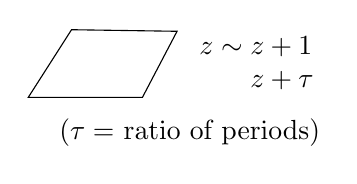
\begin{tikzpicture}[x=1cm,y=1cm,line cap=round]
\draw (0,0)--(1.45,0)--(1.89,.84)--(.55,.86)--cycle;
\node[anchor=west,align=left] at (2.05,.43) {$z\sim z+1$\\\phantom{$z\sim{}$}$z+\tau$};
\node[align=center] at (2.05,-.45) {$(\tau=$ ratio of periods$)$};
\end{tikzpicture}}\endgroup}\par\smallskip}
\end{GelfandAdjacentEvidence}
\begin{GelfandAdjacentEvidence}{GELFAND-P001249}{7}

The moduli space is not the whole upper half-plane.
\SourceFigure{GELFAND-P001249}{equivalent-parallelograms}{%
\par\smallskip
{\color{black}\begingroup\color{black}\GelfandFitDiagram{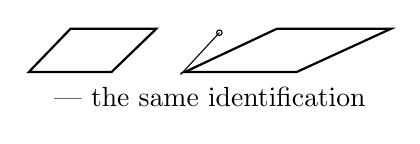
\begin{tikzpicture}[x=1cm,y=1cm,line cap=round]
\draw[thick] (0,0)--(1.05,0)--(1.62,.55)--(.53,.55)--cycle;
\draw[thick] (1.98,0)--(3.40,0)--(4.60,.55)--(3.15,.55)--cycle;
\draw[thin] (1.93,-.03)--(2.42,.50);
\draw[thin] (2.42,.50) circle (.035);
\node[align=center] at (2.30,-.32) {— the same identification};
\end{tikzpicture}}\endgroup}\par\smallskip}
\end{GelfandAdjacentEvidence}
\begin{GelfandAdjacentEvidence}{GELFAND-P001249}{8}

\begin{equation*}
\text{Transformation}\quad
\tau\longmapsto\frac{m_1\tau+n_1}{m_2\tau+n_2}\tag{8}
\end{equation*}
or
\begin{equation*}
(\tau_1,\tau_2)\longmapsto(m_1\tau_1+n_1\tau_2,\ m_2\tau_1+n_2\tau_2)
\end{equation*}
matrices
\begin{equation*}
\begin{pmatrix}m_1&n_1\\m_2&n_2\end{pmatrix},
\quad m_j,n_j\text{ are integers},\quad m_1n_2-m_2n_1=1
\end{equation*}
It suffices to use $\tau\longrightarrow\tau+1$, $\tau\longrightarrow-1/\tau$.
\SourceFigure{GELFAND-P001249}{fundamental-domain}{%
\par\smallskip
{\color{black}\begingroup\color{black}\GelfandFitDiagram{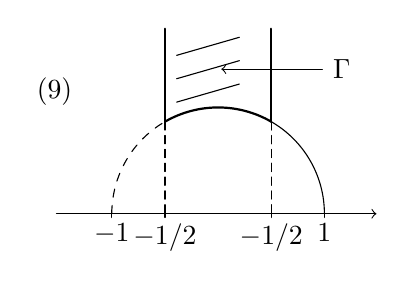
\begin{tikzpicture}[x=1.35cm,y=1.35cm,line cap=round]
\node[anchor=east] at (-1.28,1.15) {(9)};
\draw[->] (-1.52,0)--(1.49,0);
\draw[dashed] (-1,0) arc[start angle=180,end angle=120,radius=1];
\draw[thick] (-.5,.866) arc[start angle=120,end angle=60,radius=1];
\draw[thin] (.5,.866) arc[start angle=60,end angle=0,radius=1];
\draw[thick] (-.5,.866)--(-.5,1.74) (.5,.866)--(.5,1.74);
\draw[densely dashed] (-.5,.866)--(-.5,0) (.5,.866)--(.5,0);
\foreach \y in {1.05,1.27,1.49}{\draw (-.39,\y)--(.20,{\y+.17});}
\foreach \x in {-1,-.5,.5,1}
  {\draw (\x,.035)--(\x,-.035);}
\node[below] at (-1,0) {$-1$};
\node[below] at (-.5,0) {$-1/2$};
\node[below] at (.5,0) {$-1/2$};
\node[below] at (1,0) {$1$};
\draw[<-] (.03,1.36)--(.98,1.36);
\node[anchor=west] at (.99,1.36) {$\Gamma$};
\end{tikzpicture}}\endgroup}\par\smallskip}
\end{GelfandAdjacentEvidence}
\begin{GelfandAdjacentEvidence}{GELFAND-P001249}{9}

\EvidenceBlock{GELFAND-P001249}{axis-label}{The label under the right-hand vertical is also \(-1/2\).}{Manuscript notation.}
\end{GelfandAdjacentEvidence}
\begin{GelfandAdjacentEvidence}{GELFAND-P001249}{10}

$\triangle$ with angles \underline{$0^{\circ},60^{\circ},60^{\circ}$} in the Lobachevsky plane.

Consider integrals over triangle (9).

Choose a basis of holomorphic quadratic differentials on the torus
\begin{equation*}
f^1=1,\qquad \eta_1=\frac{1}{\operatorname{Im}\tau}\tag{10}
\end{equation*}
\begin{equation*}
du=dz+\delta y^1\frac{d\bar z}{\operatorname{Im}\tau}
\end{equation*}
\Unclear{GELFAND-P001249}{du-overink}{The letter after \(d\) and before the equals sign is heavily retraced. It may be \(u\) or \(y\).}
\end{GelfandAdjacentEvidence}
\begin{GelfandAdjacentEvidence}{GELFAND-P001249}{11}

[Writing before the explanation of $u$ is crossed out.]
\Incomplete{GELFAND-P001249}{u-cancel-full}{illegible crossed-out writing before the new complex symbol}
\end{GelfandAdjacentEvidence}

$u$ is a new complex coordinate (complex structure)

$y^1$ is a new coordinate in moduli space.
\begin{equation*}
\text{The matrix has exactly one entry}\quad
\frac{dy^1\wedge d\bar y^1}{\operatorname{Im}\tau}\tag{11}
\end{equation*}


\Needspace{7\baselineskip}
\begin{GelfandAdjacentEvidence}{GELFAND-P001250}{1}
\SourcePage{GELFAND-P001250}{unlabelled}
\begin{equation*}
\tau\longrightarrow\frac{u(\tau)}{u(1)}
=\frac{\tau+\dfrac{\delta y^1\bar\tau}{\operatorname{Im}\tau}}
{1+\dfrac{\delta y^1}{\operatorname{Im}\tau}}\tag{12}
\end{equation*}
\begin{equation*}
u(z)=z+\frac{\delta y^1}{\operatorname{Im}\tau}\bar z\tag{13}
\end{equation*}
$y$ gives coordinates in the space of complex structures

$y^1$ is arbitrary, $\tau$ is calculated from $y^1$
\begin{equation*}
\frac{\overline{dy^1}\wedge dy^1}{\operatorname{Im}\tau}
=\frac{d\tau\wedge d\bar\tau}{4\operatorname{Im}\tau}
\end{equation*}
\EvidenceBlock{GELFAND-P001250}{wedge-order}{The overlined differential comes first on the left and second on the right. The right denominator has \(4\) before \(\operatorname{Im}\tau\).}{Manuscript notation.}
\end{GelfandAdjacentEvidence}
\begin{GelfandAdjacentEvidence}{GELFAND-P001250}{2}


Now it remains to compute
\begin{equation*}
\int_{\Gamma}\frac{d\tau\wedge d\bar\tau}{\operatorname{Im}\tau}
\frac{\int\mathcal D X_{\mu}\,e^{\int X_{\mu}\partial\bar\partial X^{\mu}\,dz\wedge d\bar z}}
{\int\mathcal D\varepsilon\,e^{\int\bar\varepsilon\partial\bar\partial\varepsilon\,dz\wedge d\bar z}}\tag{14}
\end{equation*}
[Below the formula, an upward arrow to the measure.] $\uparrow$ (This is not the area! of the metric).
This is unsurprising, since the starting point was not invariant.

\begin{equation*}
X_{\mu}=a_{\mu}^n X^n_{\text{[\,\strut{}crossed out\,]}},
\quad \Delta X^n_{\text{[\,\strut{}crossed out\,]}}
=\lambda^n X^n_{\text{[\,\strut{}crossed out\,]}}\tag{15}
\end{equation*}
\Incomplete{GELFAND-P001250}{eigen1-underink}{illegible crossed-out subscript on the first $X^n$}
\end{GelfandAdjacentEvidence}
\begin{GelfandAdjacentEvidence}{GELFAND-P001250}{3}

\Incomplete{GELFAND-P001250}{eigen2-underink}{illegible crossed-out subscript on the second $X^n$}
\end{GelfandAdjacentEvidence}
\begin{GelfandAdjacentEvidence}{GELFAND-P001250}{4}

\Incomplete{GELFAND-P001250}{eigen3-full}{illegible crossed-out subscript on the third $X^n$}
\end{GelfandAdjacentEvidence}
\begin{GelfandAdjacentEvidence}{GELFAND-P001250}{5}

We obtain
\begin{equation*}
\frac{\int dX_{\mu}^0(\det'\Delta)^{-13}}
{\int d\varepsilon^0(\det'\Delta)^{-1}}
=\frac{V}{\operatorname{Im}\tau}(\det'\Delta)^{-12}\tag{16}
\end{equation*}
[Crossed out: Ko…]
\Incomplete{GELFAND-P001250}{cancel-word}{writing after “Ko” is crossed out and illegible}
\end{GelfandAdjacentEvidence}
\begin{GelfandAdjacentEvidence}{GELFAND-P001250}{6}

The zero-mode integrals remain.

Above is the volume of the universe (26-dimensional).

Below is the area of the torus.

Temporarily set $V=1$.

Result
\begin{equation*}
-\int_{\Gamma}
\frac{d\tau\wedge d\bar\tau}
{(\operatorname{Im}\tau)^2}(\det'\Delta)^{-12}\tag{17}
\end{equation*}
\Unclear{GELFAND-P001250}{eq17-dtau}{In (17), the head of the first \(\tau\) is heavily retraced. A separate overbar on it is uncertain.}
\end{GelfandAdjacentEvidence}
\begin{GelfandAdjacentEvidence}{GELFAND-P001250}{7}

[At bottom:] (from m.(?) parametrization) an extra $\operatorname{Im}\tau$ $\Longrightarrow$ we obtain area.
\Unclear{GELFAND-P001250}{bottom-abbrev}{The abbreviation after «из» (from) tentatively reads «м.» (m.). Its opening strokes run together and its expansion is unclear.}
\end{GelfandAdjacentEvidence}



\Needspace{7\baselineskip}
\begin{GelfandAdjacentEvidence}{GELFAND-P001251}{1}
\SourcePage{GELFAND-P001251}{59}
How to calculate
\begin{equation*}
(\det'\Delta)^{-1/2}
=\int\mathcal D\psi\,e^{-\int\partial\psi\bar\partial\psi\,dz\wedge d\bar z}\tag{18}
\end{equation*}
Calculate the variation of its $\ln$ with respect to the variation of complex structure.

$\Delta$ is the usual one, for the complex structure!
\begin{equation*}
\delta\ln(\det'\Delta)^{-1/2}\tag{19}
\end{equation*}
The idea is to use a basis in which it is diagonal, and so on.

\underline{Answer}
\begin{equation*}
\begin{aligned}
(\det'\Delta)^{-1/2}
&=(\operatorname{Im}\tau)^{-1/2}e^{\frac{\pi}{6}\operatorname{Im}\tau}
\prod_{n=1}^{\infty}\lvert1-e^{2\pi in\tau}\rvert^{-2}\\
&=(\operatorname{Im}\tau)^{-1/2}\lvert\eta(q)\rvert^{-2}
\end{aligned}\tag{20}
\end{equation*}
Use formula (18) for the calculation
\begin{equation*}
\delta(\ln\det^{-1/2}\Delta)
=\frac{\delta\int\mathcal D\psi\,e^{-\int\partial\psi\bar\partial\psi\,d^2\xi}}
{\int\mathcal D\psi\,e^{-\int\partial\psi\bar\partial\psi\,d^2\xi}}\tag{21}
\end{equation*}
[Writing after the fraction is crossed out.]
\Incomplete{GELFAND-P001251}{fraction-tail-cancel}{illegible crossed-out writing after the fraction in (21)}
\end{GelfandAdjacentEvidence}
\begin{GelfandAdjacentEvidence}{GELFAND-P001251}{2}


Here

[Writing before the variation is crossed out.]
\Incomplete{GELFAND-P001251}{metric-before-cancel}{illegible crossed-out writing before the metric variation}
\end{GelfandAdjacentEvidence}
\begin{GelfandAdjacentEvidence}{GELFAND-P001251}{3}

\begin{equation*}
\delta(\sqrt g\,g^{ab}\partial_a\psi\partial_b\psi)=\delta g^{ab}T_{ab},
\end{equation*}
where
\begin{equation*}
T_{ab}=\partial_a\psi\partial_b\psi-\frac12g_{ab}\partial^a\psi\partial^b\psi
\end{equation*}
\Incomplete{GELFAND-P001251}{stress-lower-cancel}{illegible crossed-out subscript under the superscript $a$}
\end{GelfandAdjacentEvidence}
\begin{GelfandAdjacentEvidence}{GELFAND-P001251}{4}

\EvidenceBlock{GELFAND-P001251}{stress-contraction}{The derivatives in the product after \(g_{ab}\) have superscripts \(a\) and \(b\).}{Manuscript notation.}
\end{GelfandAdjacentEvidence}
\begin{GelfandAdjacentEvidence}{GELFAND-P001251}{5}

\begin{equation*}
\delta g^{++}=\frac{\delta\tau}{\operatorname{Im}\tau},
\qquad \delta g^{--}=\frac{-\delta\bar\tau}{\operatorname{Im}\tau}
\qquad (?)
\end{equation*}
\Incomplete{GELFAND-P001251}{gpp-cancel-full}{crossed-out sign before $\operatorname{Im}$ in the denominator of $\delta g^{++}$}
\end{GelfandAdjacentEvidence}
\begin{GelfandAdjacentEvidence}{GELFAND-P001251}{6}

\Incomplete{GELFAND-P001251}{gmm-cancel-full}{crossed-out sign before $\operatorname{Im}$ in the denominator of $\delta g^{--}$}
\end{GelfandAdjacentEvidence}

Thus
\begin{equation*}
\delta(\ln\det^{-1/2}\Delta)
=2\operatorname{Re}\frac{i}{2}\delta\tau\langle T\rangle\tag{22}
\end{equation*}
where $T$ is the energy–momentum tensor,
\begin{equation*}
T(\xi)=\frac{\int\mathcal D\psi\,\partial\psi(\xi)\partial\psi(\xi)
e^{-\int\partial\psi\bar\partial\psi\,d^2\xi}}
{\int\mathcal D\psi\,e^{-\int\partial\psi\bar\partial\psi\,d^2\xi}}\tag{23}
\end{equation*}
General formula (on a surface of any genus)
\begin{equation*}
\int d^2\xi\,(\eta T+\bar\eta\bar T).\tag{24}
\end{equation*}
[At right, beyond the double vertical line.] $\partial\bar T=\bar\partial T_{+-}$.

($T$ is an almost holomorphic differential)

For a more precise form of (23), replace $\partial\psi(\xi)\partial\psi(\xi)$ by $:\partial\psi(z)\partial\psi(z):$ and take
\begin{equation*}
\begin{aligned}
T&=:\partial\psi(z)\partial\psi(z):
\overset{\mathrm{def}}{=}\oint\frac{dz'}{2\pi i}\frac{1}{z'-z}
\partial\psi(z')\partial\psi(z)\quad\overset{\text{or}}{=}\\
&=\langle\partial\psi(z)\partial\psi(z)\rangle
\overset{\mathrm{def}}{=}\biggl\langle\oint\frac{dz'}{2\pi i}\frac{1}{z'-z}
\partial\psi(z')\partial\psi(z)
\end{aligned}\tag{25}
\end{equation*}


\Needspace{7\baselineskip}
\begin{GelfandAdjacentEvidence}{GELFAND-P001252}{1}
\SourcePage{GELFAND-P001252}{unlabelled}
Formula for any genus.

There are $p$ Abelian differentials $\omega_i$ and coordinates
\begin{equation*}
\vec z(Q)=\int_{Q_0}^{Q}\vec\omega\tag{26}
\end{equation*}
\begin{equation*}
\int_{b_i}\omega_j=\tau_{ij},\qquad
\int_{a_i}\omega_j=\delta_i^j\tag{27}
\end{equation*}
Also introduce $\theta$-functions
\begin{equation*}
\theta_{\bar\varepsilon,\delta}(\vec z\mid\hat\tau)
=\sum_{\vec n}e^{\pi i\bigl(n_i\hat\tau_{ik}n_k
+2\pi i\vec z\cdot(\vec n+\vec\delta)}
\end{equation*}
\Incomplete{GELFAND-P001252}{theta-arg-cancel}{illegible crossed-out sign after the arguments of $\theta$}
\end{GelfandAdjacentEvidence}
\begin{GelfandAdjacentEvidence}{GELFAND-P001252}{2}

\Incomplete{GELFAND-P001252}{theta-exp-r2}{illegible crossed-out sign after $n_i\hat\tau_{ik}n_k$ in the first exponent}
\end{GelfandAdjacentEvidence}
\begin{GelfandAdjacentEvidence}{GELFAND-P001252}{3}

\begin{equation*}
\sum_{\vec n}e^{\pi i(\vec n+\vec\delta,\hat\tau,\vec n+\vec\delta)
+2\pi i(\vec z+\vec\varepsilon)(\vec n+\vec\delta)}
\end{equation*}
\begin{equation*}
4\vec\delta\cdot\vec\varepsilon\pmod 2
\end{equation*}
\begin{equation*}
\theta^*\equiv\theta^{\bar\varepsilon,\bar\delta}_{,k}\omega_k(z);
\end{equation*}
[Arrow to the coefficient $\theta^{\bar\varepsilon,\bar\delta}_{,k}$.]
$\longleftarrow$ \underline{derivative of $\theta$ at zero.}

[At right:] $\bar\varepsilon,\bar\delta$ is an odd characteristic.

One can take the square root of this Abelian differential (all zeros are of order 2).
\begin{equation*}
T=\frac12
\underbrace{\left[\frac{\theta^{*''}}{\theta^*}
-\frac32\left(\frac{\theta^{*'}}{\theta^*}\right)^2\right]}_{\text{Schwarzian}}
-\frac16\frac{\theta_{,ijk}\omega_i\omega_j\omega_k}{\theta'}
-\frac\pi2\omega_i(\operatorname{Im}\hat\tau)^{-1}_{ik}\omega_k
\tag{28}
\end{equation*}
\EvidenceBlock{GELFAND-P001252}{theta-stress-formula}{The first numerator reads \(\theta^{*''}\). The denominator of the next fraction reads \(\theta'\).}{Manuscript notation.}
\end{GelfandAdjacentEvidence}


All of this together is a quadratic differential.

$\omega$ does not include $dz$. The form is $\omega_i\,dz$.


\clearpage
\pdfbookmark[0]{Chapter 28}{gelfand-archive-chapter-28}
\section*{Chapter 28}
\Needspace{7\baselineskip}
\begin{GelfandAdjacentEvidence}{GELFAND-P001253}{1}
\SourcePage{GELFAND-P001253}{unlabelled}
\underline{\underline{17 Feb. 1986}}\qquad\underline{Gelfand Seminar.}

\underline{\underline{A. Beilinson}}\qquad [Crossed out: On the theory (?)] \underline{The Quillen determinant, strings, and so on.}
\Unclear{GELFAND-P001253}{title-cancel}{possibly “On the theory”}
\end{GelfandAdjacentEvidence}
\begin{GelfandAdjacentEvidence}{GELFAND-P001253}{2}


We compute the partition function
\begin{equation*}
Z=\sum_{p\geq0}Z_p.\tag{1}
\end{equation*}
$p$ is the genus
\begin{equation*}
Z_p=\int_{M_p}\mu_p,\qquad
\begin{aligned}
M_p&\text{ is the moduli space of curves of genus }p.\\
\mu_p&\text{ is the naturally arising measure}
\end{aligned}\tag{2}
\end{equation*}
For $p=1$ Kronecker (1890) and Shapiro (1972) calculated it independently (with the same result)
\begin{equation*}
\mu_1=\left|\frac{dq}{q}\right|^2\Delta(q)^{-2}\log|q|^{-13},
\qquad \Delta(q)=q\prod(1-q^n)^{24}.\tag{3}
\end{equation*}
\Unclear{GELFAND-P001253}{log-exponent}{In (3), the exponent reads \(-13\). The \(13\) above it has an arrow pointing to the exponent. The overwritten strokes and the parenthetical writing after the insertion are illegible.}
\end{GelfandAdjacentEvidence}


$\mu_1$ is a measure on the moduli space of elliptic curves

\begin{center}— . —\end{center}
$X$ is a surface of genus $p$; $g$ is a metric on $X$;
$L$ is a one-dimensional holomorphic bundle on $X$
(holomorphic structure induced by the metric), $h$ is a Hermitian metric on $L$
\begin{equation*}
\bar\partial:\Gamma(L)\longrightarrow\Gamma(L\otimes\Omega^{0,1}).\tag{4}
\end{equation*}
Then
\begin{equation*}
\underset{\substack{|\\\text{holomorphic sections}}}{H^0(X,L)}
=\operatorname{Ker}\bar\partial,\qquad
H^1(X,L)=\operatorname{Coker}\bar\partial=\operatorname{Ker}\bar\partial^{+}.
\tag{5}
\end{equation*}
(Holomorphic bundles are described by one discrete parameter, the Chern number, and $p$ continuous parameters, a point on the Jacobian.)

$H^0$, $H^1$ are finite-dimensional
\begin{equation*}
d(X,L):=\frac{\det H^0(X,L)}{\det H^1(X,L)}.\tag{6}
\end{equation*}
$\det H^0=\max$ exterior power of $H^0$ is a one-dimensional vector space

[The next line has long strokes and a repetition mark, with $H^1$ in place of $H^0$.]

Hence $d(X,L)$ is also a one-dimensional vector space.

(functions on $\det H^1$ with values in $\det H^0$)

It has a natural metric
\begin{equation*}
\begin{array}{l|l}
e_1,\ldots,e_k\text{ is a basis in }H^0&
\displaystyle d(X,L)\ni
\underset{\substack{\uparrow\\\mathbb C}}{\lambda}
\frac{e_1\wedge\cdots\wedge e_k}{g_1\wedge\cdots\wedge g_d}\\
g_1,\ldots,g_d\text{ is a basis in }H^1&
\end{array}
\end{equation*}


\Needspace{7\baselineskip}
\begin{GelfandAdjacentEvidence}{GELFAND-P001254}{1}
\SourcePage{GELFAND-P001254}{4}
The metric will be defined in two stages.

First the \underline{stupid} metric. Consider the [inserted above: natural] metric on
\Unclear{GELFAND-P001254}{top-cancel}{The crossed-out abbreviation tentatively reads «пр.» (pr.).}
\end{GelfandAdjacentEvidence}
\begin{GelfandAdjacentEvidence}{GELFAND-P001254}{2}

$\Gamma(L)$ and on $\Omega^{0,1}$,
defining pre-Hilbert structures there.

On $H^0$ and $H^1=\operatorname{Ker}\bar\partial^{+}$ metrics are also induced
$\Rightarrow$\newline
$\Rightarrow$ a metric arises in $d(X,L)$, called the stupid metric.

[Inserted above: Let us construct] \underline{the correct metric.}
[Downward arrow on the left.]

Consider $\Delta=\bar\partial^{+}\bar\partial$ and its $\det\Delta$, calculated by Belavin and Knizhnik;

$\Delta'$ is the same $\Delta$, with the zero modes removed.
\begin{equation*}
\det\Delta'=\exp\bigl(-\zeta'_{\Delta'}(0)\bigr),
\end{equation*}
\begin{equation*}
\zeta_{\Delta'}(s)=
\sum_{\substack{\lambda\in\text{eigenvalues of}\,\Delta,\\\lambda\ne0}}
\lambda^{-s},\qquad\operatorname{Re}s>1
\end{equation*}
\begin{equation*}
\begin{aligned}
&\underline{\text{Quillen metric on }d(X,L)}
\quad\left(\substack{\text{from the paper in FA}\\1985,\ N=1\ (?) }\right)\\
&\hspace{1em}=(\text{stupid metric})\cdot\sqrt{\det\Delta'}.
\end{aligned}\tag{7}
\end{equation*}
\EvidenceBlock{GELFAND-P001254}{quillen-issue}{The manuscript gives \(N=1\ (?)\), with a question mark in parentheses.}{Manuscript notation.}
\end{GelfandAdjacentEvidence}
\begin{GelfandAdjacentEvidence}{GELFAND-P001254}{3}


\underline{Explanation of definition (7).} Let
\begin{equation*}
E_1\xrightarrow{\bar\partial}E_2
\quad\text{be spaces with metrics (finite-dimensional)}\tag{8}
\end{equation*}
\begin{equation*}
d=\frac{\det\operatorname{Ker}\bar\partial}{\det\operatorname{Coker}\bar\partial}
\underset{\substack{\uparrow\\\text{canonical}\\\text{identification}}}{=}
\frac{\det E_1}{\det E_2}.\tag{9}
\end{equation*}
Let bases be given.\qquad And suppose that
\begin{equation*}
\begin{array}{l|l}
e_1,\ldots,e_k\text{ is a basis in }E_1&
\underbrace{e_1,\ldots,e_a}_{\text{basis in }\operatorname{Ker}\bar\partial}\\[2pt]
g_1,\ldots,g_{\ell}\text{ — — '' — }E_2&g_{a+1},\ldots,g_k\\
&g_{a+1}=\bar\partial e_{a+1},\ldots,g_k=\bar\partial e_k.
\end{array}\tag{10}
\end{equation*}
and
\Unclear{GELFAND-P001254}{corrected-bases}{The crossed-out product reads \(e_1\wedge\cdots\wedge e_a\). The canceled words before it are illegible. The insertion above the next line reads «соотв.». The earlier strokes above «базисов» (bases) are illegible.}
\end{GelfandAdjacentEvidence}
\begin{GelfandAdjacentEvidence}{GELFAND-P001254}{4}

the ratios of the [inserted: corresponding] bases in (9) correspond to one another.

There are metrics on the right and on the left in (9). They do not coincide — [crossed out: difference; inserted: differ] by a factor $\sqrt{\det\Delta}$

On the left is the stupid metric, and on the right the one we need, but now we define
\Unclear{GELFAND-P001254}{bottom-cancel}{The writing beneath the diagonal cancellation strokes tentatively reads «её» (yeyo).}
\end{GelfandAdjacentEvidence}

the right-hand side from the left-hand side in the infinite-dimensional situation.


\Needspace{7\baselineskip}
\begin{GelfandAdjacentEvidence}{GELFAND-P001255}{1}
\SourcePage{GELFAND-P001255}{unlabelled}
Naturality of the “correct” metric: it \underline{does not change under variation of the operator $\bar\partial$}.

In (9), if $\operatorname{Ker}\bar\partial=\operatorname{Coker}\bar\partial=0$
on the right stands $\det\bar\partial$
\begin{equation*}
\text{In general}\quad
\det(\bar\partial:E_1\to E_2)\in\frac{E_1}{E_2}
\quad\text{for one-dimensional }E_1,E_2.
\end{equation*}
\EvidenceBlock{GELFAND-P001255}{determinant-quotient}{The numerator is \(E_1\), and the denominator is \(E_2\).}{Manuscript notation.}
\end{GelfandAdjacentEvidence}
\begin{GelfandAdjacentEvidence}{GELFAND-P001255}{2}

In the infinite-dimensional case there is only the modulus of the right-hand side of (9)

\underline{Unattainable ideal:} define the right-hand side of (9) independently
\Unclear{GELFAND-P001255}{functor-cancel}{A short crossed-out passage is illegible.}
\end{GelfandAdjacentEvidence}
\begin{GelfandAdjacentEvidence}{GELFAND-P001255}{3}

of $\bar\partial$ in a functorial way (isomorphisms of spaces $\Rightarrow$ isomorphisms of determinants)

Let $L$ be the bundle of $j$-differentials, $L=\omega^j$,
its sections are $f(z)(dz)^j$.
\begin{equation*}
\begin{aligned}
&\underset{\substack{\Vert\\\rho\,dz\,d\bar z}}{\text{Riemannian metric}}
\quad\text{[crossed-out insertion: on $L$]}\\
&\qquad\text{induces a metric on }\omega^j
\quad\Rightarrow\quad \lvert(dz)^j\rvert^2=\rho^{-j}.
\end{aligned}\tag{11}
\end{equation*}
\Unclear{GELFAND-P001255}{power-cancel}{Illegible signs are crossed out after $-j$.}
\end{GelfandAdjacentEvidence}
\begin{GelfandAdjacentEvidence}{GELFAND-P001255}{4}

Here $j\in\mathbb Z$.

The space $d(x,\omega^j)$ depends only on the complex structure on $X$.

The metric $\lvert\ \rvert_j\bigl(\underset{\substack{\vert\\\text{metric on $X$}}}{\rho}\bigr)$
is the Quillen metric on $d(X,\omega^j)$

\noindent (12) \underline{Theorem} (Polyakov)
\Unclear{GELFAND-P001255}{theorem-cancel}{The crossed-out abbreviation tentatively reads «Рассм.» (Rassm.).}
\end{GelfandAdjacentEvidence}
\begin{GelfandAdjacentEvidence}{GELFAND-P001255}{5}

\begin{equation*}
\frac{\delta\bigl(\log\lvert\ \rvert_j(\rho)\bigr)}{\delta\rho}
=(6j^2-6j+1)\underset{\substack{\vert\\\text{curvature of the metric}}}{R(\rho)}
\end{equation*}

\noindent (13) Notation: $c_j=6j^2-6j+1$
\qquad (second Bernoulli polynomial)

\noindent (14) \underline{Corollary}.
Let there be a collection $j_1,\ldots,j_a\in\mathbb Z$,
[inserted above: and integers $b_1,\ldots,b_a\in\mathbb Z$,]
such that $\sum_{k=1}^{a}b_kc_{j_k}=0$.
\Unclear{GELFAND-P001255}{sum-overwrite}{The subscript on \(b\) is overwritten. The summation index \(k\) and the adjacent factor \(c_{j_k}\) support the reading \(b_k\).}
\end{GelfandAdjacentEvidence}
\begin{GelfandAdjacentEvidence}{GELFAND-P001255}{6}


Consider the Quillen metric on $\otimes\,d(X,\omega^{j_k})^{b_k}$.
\Unclear{GELFAND-P001255}{tensor-cancel}{A short crossed-out passage is illegible.}
\end{GelfandAdjacentEvidence}
\begin{GelfandAdjacentEvidence}{GELFAND-P001255}{7}

It is then independent of the [inserted: original] $\rho$,
and depends only on the complex structure on $X$

\noindent (15) \underline{Definition.} $c_j$ is called \underline{the conformal anomaly}.

\noindent (16) \underline{Most important example}.
\begin{equation*}
\begin{aligned}
j_1&=2,&b_1&=1,\\
j_2&=1,&b_2&=-13
\end{aligned}
\qquad\text{— the corresponding number }\underline{\underline{13}}
\end{equation*}
\Unclear{GELFAND-P001255}{coefficient-correction}{In $b_2$, the earlier writing after the minus sign is overwritten. The insertion above reads $13$.}
\end{GelfandAdjacentEvidence}


(In 26-dimensional space there is no conformal anomaly)
\begin{center}— . —\end{center}


\Needspace{7\baselineskip}
\begin{GelfandAdjacentEvidence}{GELFAND-P001256}{1}
\SourcePage{GELFAND-P001256}{5}
\SourceFigure{GELFAND-P001256}{family-arrow}{%
\par\smallskip
{\color{black}\begingroup\color{black}\GelfandFitDiagram{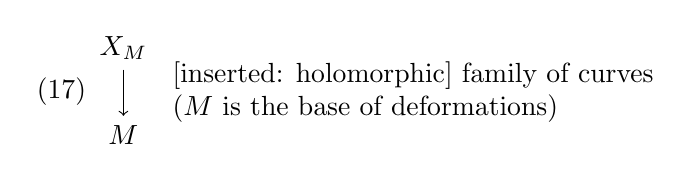
\begin{tikzpicture}[x=1cm,y=1cm]
\node[anchor=east] at (-.35,0) {(17)};
\node (total) at (0,.55) {$X_M$};
\node (base) at (0,-.55) {$M$};
\draw[->] (total)--(base);
\node[anchor=west,align=left] at (.5,0) {[inserted: holomorphic] family of curves\\($M$ is the base of deformations)};
\end{tikzpicture}}\endgroup}\par\smallskip}
\end{GelfandAdjacentEvidence}
\begin{GelfandAdjacentEvidence}{GELFAND-P001256}{2}


Then $\forall$ integer $j$ there arises a one-dimensional bundle $d_j$ over $M$
with fiber $d(X_t,\omega^j)$ over $t\in M$.

This is
\Unclear{GELFAND-P001256}{top-cancel}{Crossed out: probably “is”.}
\end{GelfandAdjacentEvidence}
\begin{GelfandAdjacentEvidence}{GELFAND-P001256}{3}

a one-dimensional holomorphic bundle over $M$.

\noindent (18)
\Unclear{GELFAND-P001256}{eq18-cancel}{Crossed out: possibly “On”.}
\end{GelfandAdjacentEvidence}
\begin{GelfandAdjacentEvidence}{GELFAND-P001256}{4}

over $\otimes\,d(X_t,\omega^{j_i})^{b_{j_i}}$ there is a canonical Hermitian metric
($b_j$ as in (14))
\EvidenceBlock{GELFAND-P001256}{eq18-index}{In (18), the exponent has the nested subscript \(b_{j_i}\).}{Manuscript notation.}
\end{GelfandAdjacentEvidence}
\begin{GelfandAdjacentEvidence}{GELFAND-P001256}{5}


\noindent (19) \underline{Theorem} (Belavin, Knizhnik):

\underline{The curvature of the canonical metric on} $\otimes\,d(X,\omega^{j_i})^{b_i}$ equals 0.

\underline{In words:} Cancellation of the conformal anomaly implies cancellation of the gravitational one.

Theorem (19) uniquely determines the [inserted: canonical] metric (which will be determined by the genus alone)
\EvidenceBlock{GELFAND-P001256}{metric-uniqueness}{The manuscript states that Theorem (19) uniquely determines the metric, with «кан.» (canonical) inserted above the line.}{Manuscript notation.}
\end{GelfandAdjacentEvidence}
\begin{GelfandAdjacentEvidence}{GELFAND-P001256}{6}


\underline{\underline{Belavin}}
\begin{equation*}
\begin{aligned}
\sum_{\text{surfaces}}e^{-a(\text{area})}
&=\sum_{p=2}^{\infty}\int d\mu_0^{(p)}
\frac{\det\Delta_{-1}^{(p)}}{(\det\Delta_0^{(p)})^{13}}\\[-1pt]
&\hspace{2em}(\text{Polyakov $+$ refinements for arbitrary genus})
\end{aligned}\tag{20}
\end{equation*}
$\Delta_j$ is the Laplacian on $j$-forms

Important: on the right is
\SourceFigure{GELFAND-P001256}{eq20-arrow}{%
\par\smallskip
{\color{black}\begingroup\color{black}\GelfandFitDiagram{\begin{tikzpicture}[x=1cm,y=1cm]
\node (fraction) at (0,1.55) {$\underbrace{\dfrac{\det\Delta_{-1}^{(p)}}{(\det\Delta_0^{(p)})^{13}}}$};
\node[draw,align=center,inner sep=4pt] (modulus) at (0,-.15) {squared modulus of a holomorphic function\\on the moduli space};
\node[align=center] (unique) at (0,-1.45) {already [inserted: almost] unique};
\draw[->] (modulus.north)--(fraction.south);
\draw[->] (modulus.south)--(unique.north);
\end{tikzpicture}}\endgroup}\par\smallskip}
\end{GelfandAdjacentEvidence}
\begin{GelfandAdjacentEvidence}{GELFAND-P001256}{7}


\begin{equation*}
\delta\bar\delta\log\det\Delta_j
=c_j\int\frac{\partial f\,\bar\partial\bar f
-f\bar f\,\partial\bar\partial\log\rho}{\rho^2},
\qquad f=\rho\eta,\tag{21}
\end{equation*}
\begin{equation*}
\delta_{\rho}\log\det\Delta_j=c_jR
\qquad\text{Variation of the metric: }dz\,d\bar z\longrightarrow\lvert dz+\eta\,d\bar z\rvert^2
\tag{21'}
\end{equation*}
\Unclear{GELFAND-P001256}{variation-cancel}{Illegible signs are crossed out above $d\bar z$ to the left of the arrow.}
\end{GelfandAdjacentEvidence}
\begin{GelfandAdjacentEvidence}{GELFAND-P001256}{8}


\underline{Beilinson}

The integral in (20) diverges and still has to be renormalized.

\underline{Belavin}
\begin{equation*}
Z_1=\int\frac{d\tau\,d\bar\tau}{(\operatorname{Im}\tau)^2}
\cdot\frac{1}{(\operatorname{Im}\tau)^{12}}\cdot\frac{1}{\lvert\Delta(q)\rvert^2},
\qquad q=e^{2\pi i\tau}
\end{equation*}
\Unclear{GELFAND-P001256}{z1-cancel}{An illegible sign is crossed out after $(\operatorname{Im}\tau)^2$ in the first denominator.}
\end{GelfandAdjacentEvidence}

The integral diverges.

But there is a conjecture that everything converges in the superstring.
\begin{equation*}
Z_2=\int\frac{d^2\tau}{(\operatorname{Im}\tau)^3}
\cdot\frac{1}{(\operatorname{Im}\tau)^{10}}\cdot\frac{1}{\lvert F(\tau)\rvert^2},
\qquad
\tau=\begin{bmatrix}\tau_{11}&\tau_{12}\\\tau_{21}&\tau_{22}\end{bmatrix}
\end{equation*}
$\tau$ is the period matrix

(Knizhnik, Morozov, Perelomov)
\begin{equation*}
F(\tau)=\prod\theta_m^2(\tau)
\end{equation*}
$Z_3$ exists as well.

For general $p$ there is no good description of the moduli space.


\Needspace{7\baselineskip}
\begin{GelfandAdjacentEvidence}{GELFAND-P001257}{1}
\SourcePage{GELFAND-P001257}{unlabelled}
\underline{Beilinson}

$M$ is the moduli space.
\[
p>2\Rightarrow\forall\ \underline{\text{holomorphic function}}=\mathrm{const}
\]

A metric [inserted above: of zero curvature] is determined up to the squared modulus of
\Unclear{GELFAND-P001257}{cancelled-word}{The crossed-out abbreviation tentatively reads «функц.» (funkts.).}
\end{GelfandAdjacentEvidence}
\begin{GelfandAdjacentEvidence}{GELFAND-P001257}{2}

a holomorphic function $\Rightarrow$ thus uniquely.
It remains to calculate it. (This reduces to calculating the unique holomorphic section
\Unclear{GELFAND-P001257}{last-line-overwrite}{There is a short overwritten mark beneath the abbreviation for “holomorphic”. Its reading is uncertain.}
\end{GelfandAdjacentEvidence}

of a certain bundle).


\Needspace{7\baselineskip}
\begin{GelfandAdjacentEvidence}{GELFAND-P001258}{1}
\SourcePage{GELFAND-P001258}{unlabelled}
\underline{24 Feb. 85.}\qquad
\underline{\underline{Kontsevich}} (\underline{Maxim}) (Gelfand Seminar)
\Unclear{GELFAND-P001258}{date-conflict}{The written date is “24/II-85.” Catalogue record 667 dates the talk to 24 February 1987.}
\end{GelfandAdjacentEvidence}
\begin{GelfandAdjacentEvidence}{GELFAND-P001258}{2}


\Unclear{GELFAND-P001258}{heading-cancel}{The canceled line shows \(\widetilde M_g\) and «пр-во бесконечномер…» (space, infinite-dimension…). The end of the word is overwritten.}
\end{GelfandAdjacentEvidence}
\begin{GelfandAdjacentEvidence}{GELFAND-P001258}{3}

$M_g$ is the space of
\Unclear{GELFAND-P001258}{moduli-cancel}{The crossed-out word tentatively reads «Модулей» (Modulei).}
\end{GelfandAdjacentEvidence}
\begin{GelfandAdjacentEvidence}{GELFAND-P001258}{4}

Teichmüller
\begin{equation*}
(\text{Curve }C,\ \text{point }p\in C,\ x\text{ is a coordinate at }p)
=\widetilde M_g
\end{equation*}
\begin{equation*}
\begin{gathered}
\mathfrak g=\mathbb C((x))\frac{\partial}{\partial x}\\
\cup\\
\mathfrak k=\mathbb C[[x]]\frac{\partial}{\partial x}
\end{gathered}
\qquad
\begin{gathered}
\gamma\text{ is the Laurent series of vector fields on }C\\
\text{with a pole at }p.\\
\gamma\subset\mathfrak g
\end{gathered}
\end{equation*}
\Unclear{GELFAND-P001258}{gamma-correction}{The first $\gamma$ is retraced and overwritten. It is repeated clearly below.}
\end{GelfandAdjacentEvidence}
\begin{GelfandAdjacentEvidence}{GELFAND-P001258}{5}

\Unclear{GELFAND-P001258}{pole-correction}{The ending of the word translated as “with a pole” is retraced and overwritten. A similar expression below supports the reading.}
\end{GelfandAdjacentEvidence}
\begin{GelfandAdjacentEvidence}{GELFAND-P001258}{6}

$\widetilde M_g$ in a neighborhood of a point is the homogeneous space $\mathfrak g/\gamma$

\noindent (1) \underline{Thm. 1.} The algebra $\mathfrak g$ acts on $\widetilde M_g$,
the stabilizer of the point [inserted above: $t$] is \(\gamma\)

Description of the action of $\mathfrak g$ on $\widetilde M_g$

Let a one-parameter family of curves be given. On this nonlinear bundle there is a connection with a pole only at the point $p$.
\SourceFigure{GELFAND-P001258}{family-sketch}{%
\par\smallskip
{\color{black}\begingroup\color{black}\GelfandFitDiagram{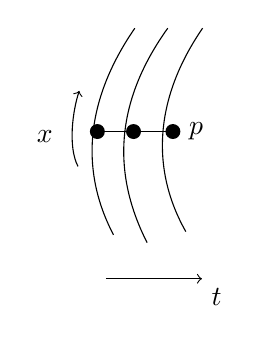
\begin{tikzpicture}[x=.82cm,y=.82cm]
\draw (0.35,0) .. controls (-0.20,1.05) and (-0.05,2.14) .. (0.68,3.2);
\draw (0.87,-0.12) .. controls (0.28,1.04) and (0.43,2.14) .. (1.19,3.2);
\draw (1.47,0.05) .. controls (0.91,1.04) and (1.00,2.14) .. (1.73,3.2);
\draw (0.10,1.60)--(1.27,1.60);
\fill (0.10,1.60) circle (2.7pt);
\fill (0.66,1.60) circle (2.7pt);
\fill (1.27,1.60) circle (2.7pt);
\node[right] at (1.37,1.60) {$p$};
\draw[->] (-.20,1.06) .. controls (-.36,1.37) and (-.28,1.93) .. (-.18,2.23);
\node[left] at (-.44,1.53) {$x$};
\draw[->] (.23,-.68)--(1.72,-.68);
\node[below right] at (1.72,-.68) {$t$};
\end{tikzpicture}}\endgroup}\par\smallskip}
\end{GelfandAdjacentEvidence}
\begin{GelfandAdjacentEvidence}{GELFAND-P001258}{7}

\begin{equation*}
\nabla_t=\frac{\partial}{\partial t}+F(x,t)\frac{\partial}{\partial x}
\end{equation*}
The tangent space to $\widetilde M_g$ is identified with $\mathfrak g/\mathfrak k$.
\EvidenceBlock{GELFAND-P001258}{tangent-quotient}{The tangent-space line reads \(\mathfrak g/\mathfrak k\).}{Manuscript notation.}
\end{GelfandAdjacentEvidence}
\begin{GelfandAdjacentEvidence}{GELFAND-P001258}{8}

\begin{equation*}
\begin{aligned}
T(\widetilde M_g)_{(C,x,p)}
&\underset{\substack{\uparrow\\\text{isomorphism}\\\text{of Kodaira–Spencer}}}{=}
\mathbb C((x))\frac{\partial}{\partial x}\big/\\[-2pt]
&\hspace{4em}\text{vector fields extending to }C\setminus\{p\}
\end{aligned}
\end{equation*}
\begin{flushright}[In the margin: (all of $C$!!)]\end{flushright}
\Unclear{GELFAND-P001258}{coordinate-corrections}{The $x$ in the Laurent series and in the derivative denominator is retraced. The earlier strokes are illegible.}
\end{GelfandAdjacentEvidence}
\begin{GelfandAdjacentEvidence}{GELFAND-P001258}{9}


$\widetilde{\mathfrak g}$ is the Virasoro algebra.
It acts
\Unclear{GELFAND-P001258}{action-cancel}{The canceled writing shows «в» (in) and \(M\) with a tilde. The subscript is overwritten and may read \(g\).}
\end{GelfandAdjacentEvidence}
\begin{GelfandAdjacentEvidence}{GELFAND-P001258}{10}

in the bundle $d_k$.
\SourceFigure{GELFAND-P001258}{lift-arrow}{%
\par\smallskip
{\color{black}\begingroup\color{black}\GelfandFitDiagram{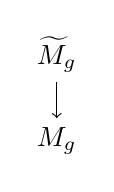
\begin{tikzpicture}[x=1cm,y=1cm]
\node (upper) at (0,.55) {$\widetilde M_g$};
\node (lower) at (0,-.55) {$M_g$};
\draw[->] (upper)--(lower);
\end{tikzpicture}}\endgroup}\par\smallskip}
\end{GelfandAdjacentEvidence}

$d_k$ is the determinant bundle over $M_g$, lifted to $\widetilde M_g$


\Needspace{7\baselineskip}
\begin{GelfandAdjacentEvidence}{GELFAND-P001259}{1}
\SourcePage{GELFAND-P001259}{unlabelled}
\underline{24 Feb. 86.}\qquad\underline{Gelfand Seminar}

\underline{\underline{Morozov}}\qquad
\underline{Consequences of the Belavin–Knizhnik theorem.}
\Unclear{GELFAND-P001259}{date-conflict}{The written date is “24.2.86.” Catalogue record 668 dates the talk to 24 February 1987.}
\end{GelfandAdjacentEvidence}
\begin{GelfandAdjacentEvidence}{GELFAND-P001259}{2}


Explicit formulas for bosonic strings, etc.

The bosonic string in the critical dimension $d=26$.

Summary of Beilinson's talk:
\EvidenceBlock{GELFAND-P001259}{continuation-note}{The first word reads «Резюме» (Summary). Strokes from the line above cross it.}{Manuscript notation.}
\end{GelfandAdjacentEvidence}
\begin{GelfandAdjacentEvidence}{GELFAND-P001259}{3}

\begin{equation*}
\begin{aligned}
&\sum_p\int Dx\,Dg\ \exp\int\sqrt g\,g^{ab}\partial_a x^\mu\partial_b x^\mu\,d^2\xi\prod_\alpha V_\alpha={}\\
&\qquad=\sum_p\int_{M_p}\frac{\lvert d\mu_p\rvert^2}{(\det\operatorname{Im}T)^{13}}\ K\{V\}
\end{aligned}\tag{1}
\end{equation*}
\EvidenceBlock{GELFAND-P001259}{det-exponent}{The heavily retraced exponent reads \(13\).}{Manuscript notation.}
\end{GelfandAdjacentEvidence}
\begin{GelfandAdjacentEvidence}{GELFAND-P001259}{4}

$V_\alpha$ are vertex operators (this will be explained later)

\SourceFigure{GELFAND-P001259}{tube-diagram}{%
\par\smallskip
{\color{black}\begingroup\color{black}\GelfandFitDiagram{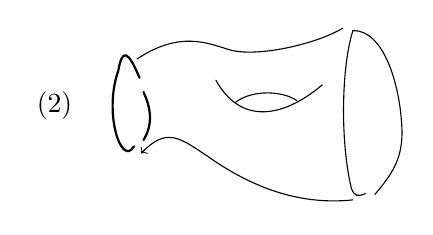
\begin{tikzpicture}[x=1cm,y=1cm,line cap=round]
\node[anchor=east] at (-.48,.12) {(2)};
\draw[thick] (.25,.47) .. controls (.10,.83) and (.03,.84) .. (-.02,.56)
  .. controls (-.21,.02) and (.02,-.67) .. (.18,-.40);
\draw[thick] (.30,.29) .. controls (.40,.08) and (.42,-.13) .. (.30,-.32);
\draw (.22,.71) .. controls (.76,1.07) and (1.12,.91) .. (1.38,.83)
  .. controls (1.73,.72) and (2.50,.90) .. (2.83,1.10);
\draw[->] (2.96,-1.08) .. controls (2.21,-1.16) and (1.59,-.86) .. (1.12,-.53)
  .. controls (.75,-.28) and (.59,-.16) .. (.27,-.49);
\draw (2.96,1.07) .. controls (2.81,.59) and (2.80,-.35) .. (2.94,-.93)
  .. controls (2.98,-1.04) and (3.02,-1.04) .. (3.12,-1.00);
\draw (2.96,1.07) .. controls (3.34,1.08) and (3.55,.42) .. (3.58,-.13)
  .. controls (3.61,-.55) and (3.45,-.76) .. (3.24,-1.01);
\draw (1.22,.44) .. controls (1.53,-.12) and (2.06,-.05) .. (2.57,.38);
\draw (1.47,.16) .. controls (1.68,.32) and (2.06,.31) .. (2.25,.18);
\end{tikzpicture}}\endgroup}\par\smallskip}
\end{GelfandAdjacentEvidence}
\begin{GelfandAdjacentEvidence}{GELFAND-P001259}{5}

\underline{worldsheet of a [raspr.] little ring}
\Unclear{GELFAND-P001259}{tube-caption}{The caption gives the abbreviation «распр.» (raspr.). Its expansion is unstated.}
\end{GelfandAdjacentEvidence}
\begin{GelfandAdjacentEvidence}{GELFAND-P001259}{6}


Mutual transformations are accounted for by considering different topologies.

Technically it is convenient to take points at the beginning and end.

\SourceFigure{GELFAND-P001259}{point-diagram}{%
\par\smallskip
{\color{black}\begingroup\color{black}\GelfandFitDiagram{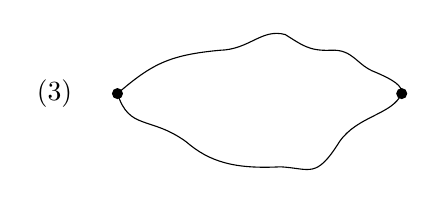
\begin{tikzpicture}[x=1cm,y=1cm,line cap=round]
\node[anchor=east] at (-.45,0) {(3)};
\draw (0,0) .. controls (.43,.37) and (.65,.49) .. (1.30,.55)
  .. controls (1.68,.56) and (1.83,.83) .. (2.13,.75)
  .. controls (2.34,.62) and (2.43,.54) .. (2.70,.55)
  .. controls (3.00,.57) and (3.03,.36) .. (3.28,.27)
  .. controls (3.51,.17) and (3.62,.10) .. (3.61,0)
  .. controls (3.49,-.27) and (3.05,-.28) .. (2.82,-.61)
  .. controls (2.52,-1.09) and (2.45,-.95) .. (2.07,-.93)
  .. controls (1.49,-.96) and (1.17,-.87) .. (.87,-.61)
  .. controls (.41,-.28) and (.15,-.47) .. (0,0);
\fill (0,0) circle (2pt);
\fill (3.61,0) circle (2pt);
\end{tikzpicture}}\endgroup}\par\smallskip}
\end{GelfandAdjacentEvidence}
\begin{GelfandAdjacentEvidence}{GELFAND-P001259}{7}

Then $V_\alpha$ are $\delta$-functions. Taking the Fourier transform, we obtain
($\alpha$ is the number of the vertex operator)
\begin{equation*}
V_\alpha(p)=\int e^{i p_\alpha x(\xi)}d^2\xi
\tag{4}
\end{equation*}
\Unclear{GELFAND-P001259}{eq4-cancel}{An illegible sign, possibly $\mu$, is crossed out after $p_\alpha$ in the exponent.}
\end{GelfandAdjacentEvidence}
\begin{GelfandAdjacentEvidence}{GELFAND-P001259}{8}


It is also convenient to take derivatives of $\delta$-functions:
\begin{equation*}
V_\alpha(p)=\int\partial x^\mu(\xi)e^{i p_\alpha x(\xi)}d^2\xi
\tag{4'}
\end{equation*}

To obtain the right-hand side of (1):

a) Integrate over $x$ to obtain
\begin{equation*}
\frac{1}{(\det\Delta_0)^{13}}\prod_\alpha\int d^2\xi_\alpha
\prod_{\alpha,\beta}\exp p_\alpha p_\beta\,G_{(reg)}(\xi_\alpha,\xi_\beta)
\tag{5}
\end{equation*}
$\Delta_0$ is the Laplacian on scalars

$G_{(reg)}$ is the regularized Green's function (smoothed when the points coincide)

\Unclear{GELFAND-P001259}{right-edge-traces}{Faint curved strokes appear in the right margin. Their reading is uncertain.}
\end{GelfandAdjacentEvidence}



\Needspace{7\baselineskip}
\begin{GelfandAdjacentEvidence}{GELFAND-P001260}{1}
